% Stanford University PhD thesis style -- modifications to the report style
% This is unofficial so you should always double check against the
% Registrar's office rules
% See http://library.stanford.edu/research/bibliography-management/latex-and-bibtex
% 
% Example of use below
% See the suthesis-2e.sty file for documentation
%
\documentclass{report}
% \setcounter{secnumdepth}{3}
% \setcounter{tocdepth}{3}
\usepackage{suthesis-2e}
\usepackage[dvipsnames,table]{xcolor}

% Math & fonts
\usepackage{amsmath, amssymb}
\usepackage{inconsolata}

% Figures and floats
\usepackage{graphicx}
\usepackage{subcaption}
\usepackage{float}
\usepackage{stfloats}
\usepackage[section]{placeins}

% Tables
\usepackage{booktabs}

% Text tweaks and structure
\usepackage{enumitem}
\usepackage{xspace}
\usepackage{microtype}

% References and links
\usepackage{cite}
\usepackage{hyperref}
\usepackage{cleveref}

% Listings
\usepackage{listings}
\usepackage{tcolorbox}

% Custom float for listings
\usepackage{newfloat}
\newfloat{lstfloat}{htbp}{lop}
\floatname{lstfloat}{Listing}
\def\lstfloatautorefname{Listing}

% Cref tweaks
% \makeatletter
% \newcommand{\nospaceS}{\S\@gobble}
% \makeatother
% \Crefname{section}{\nospaceS}{\nospaceS}
% \Crefname{figure}{Fig.}{Figs.}
% \Crefname{table}{Tab.}{Tabs.}
\Crefname{listing}{Listing}{Listings}
\crefalias{lstlisting}{listing}

% Inline code
\newcommand\code[1]{\lstinline$#1$}

% Colors
\definecolor{LighterGreen}{RGB}{190,230,190}
\definecolor{LightGreen}{RGB}{150,210,140}
\definecolor{LightRed}{RGB}{255,100,100}
\definecolor{LighterRed}{RGB}{255,150,150}
\definecolor{LightestRed}{RGB}{255,200,200}

\lstdefinelanguage{Rust} {
 keywords={fn, trait, struct, bool, u32, u64, u16, u8, usize},
 keywordstyle=\color{BrickRed}\bfseries,
 ndkeywords={QuACK, Quacker, ClientQuacker, Quack},
 ndkeywordstyle=\color{NavyBlue}\bfseries,
 basicstyle=\ttfamily,
 identifierstyle=\color{black},
 sensitive=false,
 comment=[l]{///},
 commentstyle=\color{gray}\ttfamily\bfseries,
 showstringspaces=false,
 string=[s]{"}{"},
 stringstyle=\color{ForestGreen}\ttfamily,
}

\newcommand{\gina}[1]{\textcolor{red}{\sf {(GY: #1)}}}

\dept{Computer Science}

\begin{document}
\title{In-Network Assistance for Secure Transport Protocols}
\author{Gina Yuan}
\principaladviser{Keith Winstein}
\firstreader{David Mazières}
\secondreader{Dan Boneh}
% \thirdreader{Matei Zaharia} %if needed
% \fourthreader{Severus Snape} %if needed
 
\beforepreface
%-------------------------------------------------------------------------------
\begin{abstract}
%-------------------------------------------------------------------------------

This paper describes and evaluates new techniques for
network-originated retransmissions for end-to-end transport
connections, yielding performance benefits for encrypted transport
protocols in lossy settings.  We use set-reconciliation techniques
based on the Rateless IBLT to let the receiver efficiently acknowledge
encrypted packets to a network function, without modifying the sender
or the underlying wire format. With these tools, endpoints can receive
network-originated retransmissions appropriate for them, without an
additional layer of encapsulation, tunnel, or link-layer
retransmissions.

% Lossy network paths can significantly harm application performance. Existing
% approaches such as link-layer retransmissions and connection-splitting either
% cannot be tuned to the connections that share the link, or are otherwise
% infeasible without ossification or credentialing the proxy. In this paper, we
% show how in-network retransmissions via a sidekick connection can enable a
% variety of performance enhancements---higher throughput, lower latency, and
% lower link overheads---for a variety of \textit{encrypted} transport protocols
% in these settings. We utilize set reconciliation techniques based on the quACK
% to refer to encrypted packets, without involving the data sender, and leave the
% underlying protocol unchanged on the wire and opaque to the
% performance-enhancing proxy.

% These in-network retransmissions require an on-path proxy located near the
% data \textit{receiver}, and scalability becomes challenging when the more
% complex decoding and retransmission logic is shifted from the endpoint to the
% proxy. To address this issue, we present an alternate construction of the quACK
% using the IBLT data structure, improving the efficiency of encoding and
% decoding operations. Combined with the insight that the quACK sender is
% co-located at the endpoint with the application ACK sender, we can send
% significantly fewer and smaller quACKs overall, minimizing the extra load
% introduced by the sidekick connection to the network.

\end{abstract}

\prefacesection{Quacknowledgments}
I would like to thank...

(advisor)
Keith Winstein.

(mentors)
Michael Welzl.
Matei Zaharia, David Mazières.

(more mentors)
Dan Boneh, Mary Wootters.
Te-Yuan Huang, Deian Stefan, Wei Wei, Yiannis Yiakoumis, Bruce Spang.
Robert Morris, Malte Schwarzkopf, Jon Gjengset, Raul Castro Fernandez, Albert
Carter.
As I mature as a researcher, I gain perspective.
It feels like they saw something in me that I didn't see yet.

(collaborators) Matthew Sotoudeh, David Zhang. Thea Rossman.

(SNR) Yuhan Deng, Akshay Srivatsan, Colin Drewes,
Yasmine Mitchell, Francis Chua, Sebastian Ingino, Angie Montemayor.
Boba, crosswords, hang gliding, sailing and water activities, bike rides,
systems lunch, hackathon.

(DAWN) Liana Patel, Pratiksha Thaker, Kexin Rong, Sahaana Suri, Keshav
Santhanam, Fiodar Kazhamiaka, James Thomas, Peter Kraft, Qian Li, Daniel Kang,
Omar Khattab, Trevor Gale, Kai Sheng Tai, Firas Abuzaid, Lingjiao Chen, Cody
Coleman, Jared Quincy Davis, Deepti Raghavan, Deepak Narayanan, Shoumik Palkar.
(special thanks) Deepti, Deepak, Shoumik.

(Stanford community) Evan Laufer, Geoffrey Ramseyer, Zachary Yedidia, Chaeyoung
Lee, Yu-Neng Wang, Pu (Luke) Yi, Sally Wang, AJ Root, Anjiang Wei, Shiv
Sundram, Alex Ozdemir, Agur Adams, Yao Hsiao, Rohit Nema. Aishwarya Mandyam.
Coach Adrian Bennett, Miles Chan, Claire MacDougall, Paddy Simha.
Coach Isaiah Newkirk, Kelly Brennan. Albert Wu, Basil Saeed,
Ying-Yu Ho, Jack Liu.

(NCNCA cycling) Niky Taylor. Chloé Mauvais. Prof. Kate Maher, Ilan Jen-La
Plante, Alex Obrand. Sue Lin Holt, Robin Betz, Ari Fischer, Emily Schell,
Louise Thomas, Steph Hart, Rachel Hwang, Katie Monaghan. Alto Velo community
and the Egan ride.

% Hoss Hayati, Will Hakim, Cam O'Reilly, Simon Parton, Tony Gallagher.

(family)
Christine Lei, Wei Yuan. Paula Yuan. Weijiu Zhang.

(partner)
Jack Liu. Hanji and Tater.

\afterpreface

\section{Introduction}
\label{sec:sidekick:intro}

In the Internet's canonical model, transport is end-to-end and implemented only
in hosts. Traditionally, routers and other network components forwarded IP
datagrams without regard to their payloads or flow membership~\cite
{saltzer1984endtoend, clark1988darpa}; only hosts thought about connections,
reliable delivery, or flow-by-flow congestion control.

In practice, however, the best behavior for a transport protocol depends on the
particulars of the network path. An appropriate retransmission or
congestion-control scheme for a heavily-multiplexed wired network wouldn't be
ideal for paths that include a high-delay satellite link, Wi-Fi with bulk ACKs
and frequent reordering, or a cellular WWAN~\cite
{kuhn2021quic-over-sat,goyal2017abc}.

By the 1990s, many networks had broken from the canonical model by deploying
in-network TCP accelerators, also known as ``performance-enhancing proxies''
(PEPs)~\cite{rfc3135}. TCP PEPs can split an end-to-end connection into
multiple concatenated connections~\cite
{kapoor2005achieving,caini2006pepsal,davern2011httpep,farkas2012splittcp,hayes2019mmwave},
buffer and retransmit packets over a lossy link~\cite
{balakrishnan1995snoop,polese2017milliproxy}, virtualize congestion
control~\cite{cronkite2016vcc,he2016acdc,mihaly2012mobilePEP}, resegment the
byte stream, and enable forward error correction, explicit congestion
notification, or other segment-specific enhancements. Because TCP isn't
encrypted or authenticated, PEPs can achieve this transparently, without the
knowledge or cooperation of end hosts. Roughly 20--40\% of Internet paths cross
at least one TCP PEP~\cite{imc2011handley, edeline2019bottomup}.

While many flows benefit from PEPs, their use carries a cost: protocol
ossification~\cite{papastergiou2017deossifying, edeline2019bottomup}. When a
middlebox inserts itself in a connection and enforces its preconceptions about
the transport protocol, it can thwart the protocol's evolution, dropping
traffic that uses an upgraded version or new options. TCP PEPs have hindered or
complicated the deployment of many TCP improvements, such as ECN++, tcpcrypt,
TCP extended options, and multipath TCP~\cite
{mandalari2018ecnplusplus,imc2011handley,raiciu2012multipathtcp}.

In response to this ossification, and to an increased emphasis on privacy and
security, post-TCP transport protocols have been designed to be impervious to
meddling middleboxes, by encrypting and authenticating the transport header. We
refer to these newer transport protocols as ``secure'' transport protocols. The
most prevalent is QUIC~\cite{rfc9000}, found in billions of installed Web
browsers and millions of servers~\cite{zirngibl2021quicdeployment}; other secure
transport protocols are used in WebRTC/SRTP~\cite{rfc8834webrtc},
Zoom~\cite{zoom}, BitTorrent~\cite{bittorrent}, and
Mosh/SSP~\cite{winstein2012mosh}.

This encryption means that middleboxes can't interpose themselves on a
connection or understand the sequence numbers of packets in transit. This
prevents PEPs from providing assistance, reducing---in some situations---the
performance of secure transport protocols~\cite
{border2020quicsat-presentation,kuhn2021quic-over-sat,martin2022bbr-quic-sat,border2020evaluating,kosek2022quicpep}.
It's possible to co-design protocols and PEPs to preserve security and privacy
while permitting assistance from credentialed middleboxes~\cite
{ford2008logjam,sherry2015blindbox, dogar2012tapa,iyengar2009flow}, but
challenging to do so without tightly coupling these components, risking
ossification and fragility.

In this chapter, we propose a method for in-network assistance of secure transport
protocols that tries to resolve this tension. Our approach leaves the transport
protocol unchanged on the wire: an encrypted end-to-end connection between hosts,
opaque to middleboxes and free to evolve. No PEPs are credentialed to decrypt
the transport protocol's headers.

Instead, we propose a second protocol to be spoken on an adjacent connection
between an end host and a PEP. We call this the \emph{\bf Sidekick protocol},
and its contents are \emph{about} the packets of the underlying, or ``base,''
connection. Sidekick PEPs assist end hosts by reporting what they've observed
about the packets of the encrypted base connection, without coupling their
assistance to the details of the base protocol. End hosts use this information
to influence decisions about how and when to send or resend packets on the base
connection, approximating some of the performance benefits of traditional PEPs.
We first proposed a similar functional separation in \cite{yuan2022sidecar},
and presented a concrete realization of the idea and its nuanced
interactions with real transport protocols in \cite{yuan2024sidekick}.

One key technical challenge with this approach is how the Sidekick can
efficiently refer to ranges of packets in an encrypted base connection. These
packets appear random to the middlebox, and referring to a range of, e.g., 100
encrypted packets in the presence of loss and reordering is not as simple as
saying ``up to 100'' when there are cleartext sequence numbers. In \Cref
{sec:quack}, we presented and evaluated a mathematical tool called a \emph
{\bf quACK} that concisely represents a selective acknowledgment of randomly
encrypted packets. In this chapter, we leverage the power sum quACK,
based on the insight that we can model the problem as a system of power
sum polynomial equations if there is a practical bound on the maximum number of
``holes'' among the packets being ACKed.

A second challenge is how the end host should use information from a Sidekick
connection to obtain a performance benefit for its base connection. Since the
performance benefit comes from changing behavior at the end host rather than
the middlebox, transport protocols need to incorporate this information into
their existing algorithms for, e.g., loss detection and retransmission, which
have gotten increasingly complex over time. To explore this, we designed a
Sidekick protocol and integrated it into client implementations in three scenarios:
\begin{itemize}[noitemsep,topsep=2pt]
\item A low-latency audio stream over an Internet path that includes a Wi-Fi path segment
  (low latency with loss), followed by a WAN path segment (higher latency
  with low loss). Can the Sidekick PEP reduce the de-jitter buffer delay
  by triggering earlier retransmissions on loss?

\item An upload over the same path. Can a secure transport protocol like QUIC,
  aided by a Sidekick PEP at the point between these two path segments, match
  the throughput of TCP over a connection-splitting PEP?

\item A battery-powered receiver, downloading data from the Internet over Wi-Fi.
  If the Wi-Fi access point sends Sidekick quACKs on behalf of the receiver,
  can it reduce the number of times the receiver's radio needs to wake up
  to send an end-to-end ACK?
\end{itemize}

\smallskip

A third technical challenge is how knowledge about \emph{where}
loss occurs along a path should influence a congestion-control scheme.
The challenge in any such scheme is how to maximize the congestion window
while sharing the network fairly with competing flows.
We present a path-aware modification to the CUBIC congestion-control
algorithm~\cite{ha2008cubic}, which we call \mbox{\textbf{PACUBIC}},
that approximates the congestion-control behavior of a PEP-assisted split TCP
CUBIC connection while making its decisions entirely on the host.

\paragraph{Summary of results.}

We implemented the Sidekick protocol in a low-latency media client
based on the WebRTC standard, and an HTTP/3 client using the Cloudflare
implementation of QUIC~\cite{quiche} and the \texttt{libcurl}~\cite{libcurl}
implementation of HTTP/3. We evaluated the three scenarios in
real-world and emulation experiments.
In real-world experiments using an unmodified local Wi-Fi network to access our
nearest AWS datacenter, the Sidekick was able to trigger early retransmissions
to fill in gaps in the audio of a latency-sensitive audio stream, reducing the
receiver's de-jitter delay from 2.3~seconds to 204~ms---about a 91\% reduction
(\Cref{fig:real-world}). The Sidekick was also able to improve the speed of an
HTTP/3 (QUIC) upload by about 50\%.

In emulation experiments of the ``battery-powered receiver'' scenario,
the Sidekick PEP was able to reduce the need for the receiver to send ACKs
by sending proxy acknowledgments on its behalf---ACKs the sender used
to advance its flow-control and congestion-control windows. The
receiver only needed to wake up its radio to send occasional
end-to-end ACKs, which the sender used to discard data from its
buffer (\Cref{fig:ack-reduction}).

Also in an emulation experiment, we confirmed that PACUBIC's
performance approximates a split CUBIC connection (two TCP CUBIC
connections separated by a PEP), responding to loss events on the
different path segments similarly to how the individual CUBIC flows would
(\Cref{fig:loss-vs-tput}). The results indicate that the Sidekick protocol's gains
do not come at the
expense of congestion-control fairness relative to a split CUBIC connection.

\smallskip

The rest of this chapter discusses three motivating scenarios for the Sidekick
(\Cref{sec:sidekick:motivating}), describes the concrete Sidekick protocol we
built around power sum quACKs (\Cref{sec:sidekick:init,sec:sidekick:sender}) and
its implementation in two base protocols (\Cref{sec:sidekick:implementation}),
and then evaluates the protocol in real-world (\Cref{sec:sidekick:real-world})
and emulation experiments (\Cref{sec:sidekick:emulation}).

\chapter{QuACKs}
\label{sec:quack}

In a Sidekick connection, a proxy needs to be able to refer to and efficiently
acknowledge a set of packets even when they are randomly encrypted. Since
packets in a TCP connection are labeled with cleartext sequence numbers, it is
straightforward to refer to a set of TCP packets using cumulative and selective
ACKs. But this problem is technically challenging for packets of secure
transport protocols without access to cleartext sequence numbers or the
ossification of other fields.

We mathematically define the quACK problem in the context of network packets
sent over a lossy path segment, and discuss how to select \emph{identifiers} to
refer to encrypted packets. We analyze strawman solutions to the quACK problem
that use either too much space or computation. Then, we present two efficient
constructions of the quACK inspired by related theoretical work in set
reconciliation~\cite{minsky2003set,eppstein2011straggler}, as well as coding
theory and graph theory~\cite{karpovsky2003data}. Both constructions require a
bound on the maximum number of missing elements, a threshold $t$, and have
different tradeoffs. The \textit{power sum} construction is space-optimal and
deterministic, but requires an exact bound. The \textit{invertible Bloom lookup
table (IBLT)} construction is more computationally scalable with an approximate
bound, but also probabilistic with constant factor overheads.

Concretely realized, the power sum quACK uses 48~bytes to express the equivalent
of TCP's cumulative + selective ACK over the 32-bit identifiers of randomly
encrypted packets, tolerating up to 10 missing packets before the last
``selective ACK.'' On a recent x86-64 CPU, it takes 26~ns to encode a single
packet in the power sum quACK, and 15.5~$\mu$s to decode which received packets
the quACK represents. The IBLT quACK takes 42~ns to encode a single packet and
1.3~$\mu$s to decode a quACK, using at least 58~bytes. These overheads compared
well with several alternatives
(\Cref{tab:quack:overview:practical}).

\section{The QuACK Problem}
\label{sec:quack:problem}

In the quACK problem, a sender (such as an endpoint) transmits a
multiset\footnote{A ``multiset'' means the same element can be transmitted more
than once.} of elements $S$. At any given time, a receiver (such as a proxy)
has received a subset $R \subseteq S$ of the sent elements. We would like the
receiver to communicate a small amount of information to the sender, who then
efficiently decodes the missing elements---the set difference $S \setminus
R$---knowing $S$. This small amount of information is called the ``quACK''. The
problem is: \textbf{what is in a quACK and how do we decode it?}

\subsection{Identifiers}
\label{sec:quack:problem:identifiers}

How exactly do we refer to the elements in the quACK problem that have been sent
or received? In a networking context, these elements are packets. Traditional
TCP proxies have been able to interpose their own concise, cumulative
acknowledgments using cleartext sequence numbers, but this is not possible with
modern, secure transport protocols. Even if a connection did expose an
unencrypted numerical field, we would not want to refer to that field at risk
of ossifying that protocol.

Instead, we need a function that deterministically maps
a packet to a random $b$-byte \emph{identifier}. The most trivial solution
that applies to all base protocols is
to hash the entire payload. Another option if the payload is already
pseudorandom (e.g., QUIC) is to take the first $b$ bytes from a fixed
offset of that payload. Although the latter option would rely on those bytes
to remain pseudorandom, it is computationally more efficient because it
does not require reading the entire payload.

\subsubsection{Collisions.}
The main considerations when selecting the number of bytes, $b$, in an
identifier is the tolerance for collisions compared with the extra data
needed to refer to these packets on the link. The larger $b$ is, the lower
the collision probability but the greater the link overhead.

Define the collision probability to be the probability that a randomly-chosen
$b$-byte identifier in a list of $n$ packets maps to more than one packet in
that list.
If we assume that identifiers are uniformly distributed,
this probability is equal to $1-(1 - 1/256^{b})^{n-1}$.
When $n=500$, using $4$ bytes results in an almost negligible
chance of collision while using $2$ bytes results in a 0.8\% chance
(\Cref{tab:quack:collision-prob}).

\begin{table}[ht]
  \centering
  \begin{tabular}{|l|l|l|l|l|}
    \hline
    \textbf{Identifier Bytes} & 1 & 2 & 4 & 8 \\
    \hline
    \textbf{Collision Prob.}
    & 0.090 & 0.0004 & $5.6\text{e-09}$ & ${\approx}0$ \\
    \hline
  \end{tabular}
  \caption{Collision probabilities for $n=25$.
  }
  \label{tab:collision-prob}
\end{table}


When handling collisions, a sender who is decoding a quACK has a list of $n$
packets it is trying to classify as received or missing
(\Cref{sec:quack:constructions}). This is the number of packets that were either
not classified or newly transmitted since decoding a previous quACK.
Note that collisions are also known to the
sender beforehand. If there is a collision between a packet that is received
and a packet that is missing, the fate of that identifier is considered
indeterminate. Either the protocol can still function with approximate
statistics (e.g., congestion control) or it can fall back to an end-to-end
mechanism (e.g., retransmission).

\subsection{Strawman solutions}
\label{sec:quack:problem:strawmen}

A problem that is simple with cumulative and selective acknowledgments of
plaintext sequence numbers is deceivingly challenging for pseudorandom
packet identifiers. Consider the following strawman solutions to the quACK
problem:

\subsubsection{Strawman 1: Echo every identifier.}
Strawman 1a, similar to \cite{li-tsvwg-loops-problem-opportunities-06,kramer2020lwpep},
echoes the identifier of every received packet in a new UDP packet to the data
sender.  Decoding is trivial given that the identifiers are unmodified.
This strawman adds significant link overhead in terms of additional packets.
Additionally, since the strawman is not cumulative, losing a quACK means the
end host could falsely consider a packet to be lost, creating a congestion
event or spurious retransmission.

Strawman 1b echoes a sliding window of identifiers over UDP such that there is
overlap in the identifiers referred to by consecutive quACKs.
This solution is slightly more resilient to loss, but uses more bytes and is
still not guaranteed to be reliable.
Another variant batches identifiers to reduce the number of packets, but this
solution is even less resilient to loss.

We also consider a Strawman 1c that echoes every identifier over TCP with
\texttt{TCP\_NODELAY} to send every identifier in its own packet.
This ensures there are no false positives when detecting lost packets,
but adds even more link overhead in terms of TCP headers and additional ACKs
from the data sender (every other packet by default in the Linux kernel).

\subsubsection{Strawman 2: Cumulative hash of all identifiers.}
Strawman 2 sends a SHA-256 hash of a sorted concatenation of all the received
packets in a UDP packet, and the sender hashes every subset of the same size of
sent packets until it finds the subset with the same hash (assuming collision
resistance). The strawman includes a count of the packets received to determine
the size of the subset to hash. As the number of missing packets exceeds even a
moderate amount, the number of subsets to calculate a hash for explodes, making
the strawman impractical to decode.\\

\noindent
One might also suggest the receiver send negative acknowledgments of the packets
it has not received. However, unlike sequence numbers where one can
determine a gap in received packets, there is no way to tell with random
identifiers what packet is missing or should be expected next.

\section{Efficient constructions of the quACK in packet-scale settings}
\label{sec:quack:constructions}

The problem of providing a concise acknowledgment of encrypted packet
identifiers closely resembles a more general problem called set reconciliation.
In this problem, two parties, each with a set, communicate a small amount of
information to learn the set difference---the elements missing in the other
set~\cite{minsky2003set,eppstein2011straggler}. There are two well-known classes
of solutions to this set reconciliation problem with different tradeoffs
in communication and computation cost.
We provide background in the literature on the set reconciliation problem,
then describe the efficient power sum and invertible Bloom lookup table (IBLT)
constructions of the quACK based on these two classes of solutions
(\Cref{tab:quack:constructions}).

\begin{table}[t]
  \centering
  % \renewcommand{\arraystretch}{0.000023}
  \begin{tabular}{ll}
    \toprule
    \bf Construction & \bf Description \\
    \midrule
    Strawman 1a & Echo every identifier. \\
    Strawman 1b & Echo a sliding window of identifiers. \\
    Strawman 1c & Echo every identifier over TCP. \\
    Strawman 2 & Hash a sorted concatenation of all identifiers.\\
    \rowcolor{yellow}
    \bf Power Sums & Encode the identifiers in symmetric power sum polynomial equations. \\
    \rowcolor{yellow}
    \bf IBLT & Map the identifiers to cells in an invertible Bloom lookup table data structure. \\
    \bottomrule
  \end{tabular}
  \caption{
  Descriptions of the strawman and set-reconciliation-based quACK constructions.
  }
  \label{tab:quack:constructions}
\end{table}


\subsection{Background: Set reconciliation}
\label{sec:quack:constructions:background}

The first class of solutions models the problem as a system of symmetric power
sum polynomial equations. This construction is deterministic as the set
difference is just the solutions to this system of equations. It is also
space-optimal; \cite{minsky2003set} introduced symmetric polynomials as a
solution to the set reconciliation problem with nearly optimal communication
and tractable computation cost. \cite{dodis2004fuzzy} improved the computation
cost in decoding, but found the problem to be intractable for larger parameters.
The power sum solution has mainly been restricted to more theoretical
literature.

The second class of solutions encodes the elements in an Invertible Bloom Lookup
Table (IBLT), and is more computationally scalable than the first class. The
IBLT is a data structure based on the Bloom
filter~\cite{goodrich2011invertible}, and probabilistically decodes the set
difference with a multiplicative factor on the comunication cost. This
multiplicative factor has been shown to be small on average: $1.23$\footnote{The
$1.23\times$ multiplicative factor on the communication cost is derived from
$1/\alpha$, where $\alpha \approx 0.81$ in
\cite{baek2023simple}.}--$1.35\times$~\cite{yang2024practical,baek2023simple}.
In practice, set reconciliation with a Bloom-filter-like data structure has
mainly been applied to larger distributed systems such as blockchain and social
media synchronization~\cite{yang2024practical,summermatter2021byzantine}.

The quACK setting differs from previous applications of set reconciliation in
several ways. In this setting, the elements in the problem are network packets,
or more specifically packet \textit{identifiers}. Only the receiver
communicates information, and the sender performs subset and not set
reconciliation on the missing packets. Unlike the blockchain setting, the two
parties synchronize on millisecond-RTT timescales compared to seconds. The
communication must be encoded in a single network packet, not a stream of
packets. In addition, at these smaller timescales, fewer elements
(typically tens) are reconciled at once, and optimizations for constant factor
overheads matter more.

\subsection{Power sums: A space-optimal and deterministic solution}
\label{sec:quack:constructions:power-sum}

We describe a construction of the quACK that models the problem as a system of
power sum polynomial equations when we have an exact bound on the maximum
number of missing elements, a threshold $t$. Unlike the previous strawmen, this
construction is efficient to decode, and its size is proportional only to $t$.

Consider the simplest case, when the receiver is only missing a single element.
The receiver maps packet identifiers to a finite field,
i.e. modulo the largest prime that fits in $b$ bytes,
 and communicates the sum $\sum_{x \in R} x$ of the received
elements to
the sender. The sender computes the sum $\sum_{x \in S} x$ of the sent elements
and subtracts the sum from the receiver, calculating:
\[
    \sum_{x \in S} x - \sum_{x \in R} x = \sum_{x \in S\setminus R} x,
\]
which is the sum of elements in the set difference. In the case of a single
missing element, the sum is exactly the value of the missing element.

In fact, we can generalize this scheme to any number of missing elements $m$.
Instead of transmitting only a single sum, the receiver communicates
the first $m$ \emph{power sums} to the sender, where the $i$-th power sum of a
multiset $R$ is defined as $\sum_{x \in R} x^i$.
The sender then computes the first $m$ power sums of $S$ and calculates the
respective differences $d_i$ for $i \in [1,m]$, producing the following
system of $m$ equations:
\[
    \left\{\, \sum_{x \in S\setminus R} x^i = d_i \mid i \in [1,m] \right\}.
\]

Instead of transmitting an unbounded number of power sums, the receiver only
maintains and sends the first $t$ power sums. Efficiently solving these $t$
power sum polynomial equations in $t$ variables in a finite field is a
well-understood algebra problem~\cite{eppstein2011straggler}. The solutions are
exactly $x \in S \setminus R$.

\subsection{Invertible Bloom lookup table: A computationally scalable approach}
\label{sec:quack:constructions:iblt}

Now we apply the IBLT to describe a probabilistic construction of the quACK in
a Bloom-filter-like data structure. The IBLT construction has better computation
complexity than the power sum construction, but incurs higher constant factor
overheads and is probabilistic.
Recall that the IBLT data structure consists of some number of cells, where each
cell contains an XOR and a count of elements in the cell. In the IBLT, $t$ is
only an approximate bound on the number of missing elements, so we set the
number of cells to some multiplicative factor more than $t$.

When the sender or receiver adds an element to the IBLT, we leverage the
pseudorandom mapping algorithm of the Rateless IBLT to determine which cells
to update~\cite{yang2024practical}. This algorithm maps each element to
$O(\log(t))$ cells, with a greater density in the cells with smaller indexes.
This resembles rateless error-correcting codes with an infinite stream of coded
symbols in that a prefix of an IBLT with an infinite number of cells can be
used to deterministically decode the elements in the IBLT.

The IBLT also allows the removal of elements and subtraction of two IBLTs with
the same number of cells. To find the set difference between the elements in
two IBLTs, we first ``subtract'' the corresponding XORs and counts. To decode
the elements encoded in the difference IBLT, we remove elements from cells with
a count of 1 until no such cells remain. (Note that the count cannot be
negative with subset reconciliation.) Decoding is successful if all counts
and XORs are 0 at the end, and can fail probabilistically due to collisions in
the mapping algorithm.

\section{Implementation}
\label{sec:quack:implementation}

The implementation of the quACK must be practical for packet-scale settings. The
communication must fit in a single network packet, ideally even less to be
considered a control packet for congestion control purposes. For example, a TCP
ACK is only 20 bytes on the wire, excluding Ethernet and IP headers.
The implementation should also provide a convenient interface to
interchangeably use different constructions of the quACK.

We define a common API for quACK implementations, shown in
\Cref{lst:quack:api}. Our optimized implementations of the power sum and
IBLT quACK constructions adhere to this interface and are available as a
software library at \url{https://www.github.com/ygina/quack}.
The computation costs are practical for decoding set differences at
millisecond-RTT timescales and encoding packets when they arrive every few
nanoseconds (\Cref{tab:quack:overview:practical}).

\subsection{Wire format}

The wire format of the quACK reflects its communication cost in a Sidekick
connection. Although the actual mechanism in which quACKs are transmitted over
the wire is not tied to the design, we assume quACKs to be written in the
payload of a UDP datagram, possibly with a small header. Assuming we use 32-bit
integers as packet identifiers, the actual quACK consists of three fields:

\begin{enumerate}[label=(\roman*),noitemsep]
\item The 4-byte count of received elements,
\item The 4-byte identifier of the last element received, and
\item $t$ symbols, where $t$ determines the number of missing elements that can
 be decoded.
\end{enumerate}

The count and last element received are valuable for efficient decoding in the
quACK context. The sender uses the count to calculate the number of missing
packets $m$, which is not known ahead of time, by subtracting the count of the
quACK transmitted by the receiver from its own count. The last element received
is an optimization that allows $m$ to represent just the ``holes'' among the
packets being selectively ACKed, excluding the consecutive elements that are
in-flight (\Cref{sec:sidekick:sender:loss-detection}).

The wire format of the symbol depends on the construction of the quACK. In the
power sum construction, the symbol is just a power sum of the elements, and
uses 4 bytes. In the IBLT construction, the symbol consists of both an XOR of
the elements and a count. With 4-byte identifiers, the count uses just one byte
for a total of 5 bytes. The total communication cost of the quACK (excluding
headers) is either $8+4\cdot t$ or $8+5\cdot t$ bytes, depending on the
construction.

\subsubsection{Why is a single byte sufficient for the count in an IBLT cell?}

Note that a quACK needs to fit in a single UDP datagram, which limits us to
$\approx\!1400$ bytes excluding headers. If each XOR is $4$ bytes, then there
can be at most $350$ packets in the set difference. Note that $8$-byte
identifiers are unnecessary because collisions are unlikely in these small set
difference sizes. The count in each symbol needs to be as large as the set
difference size. It can also be an unsigned integer because we do subset
(and not set) reconciliation, and we can subtract with overflow. An 8-bit
integer goes up to $255$, which is sufficiently close. Thus the largest IBLT
quACK contains $255$ symbols or $4 + 4 + 255 \cdot 5 = 1283$ bytes on the wire.

\subsection{QuACK API}

\begin{lstfloat}[t]
\begin{lstlisting}[language=Rust]
trait quACK {
    fn count() -> usize;
    fn last_identifier() -> u32;
    fn encode(item: u32);
    fn remove(item: u32);
    fn sub(rhs: quACK) -> quACK;
    fn decode() -> &[u32];
}
\end{lstlisting}
\captionof{lstlisting}{Pseudocode interface for the implementation of the quACK
 in the \texttt{quack} library. Each item is a 4-byte random identifier
 referring to a network packet.}
\label{lst:quack:api}
\end{lstfloat}


The API for the quACK consists of the basic operations for encoding and
decoding elements as described in \Cref{sec:quack:constructions}
(\Cref{lst:quack:api}). The
\texttt{encode()} and \texttt{remove()} functions add and remove a single
element, respectively, either by updating all power sums or by updating the XOR
and counts in the mapped IBLT cells. The \texttt{sub()} function calculates the
set difference between two quACKs, and the \texttt{decode()} function returns
the decoded elements in that set difference. The values returned by the
\texttt{count()} and \texttt{last\_element()} functions are incrementally
updated as elements are added and removed.

We explored many optimizations to improve the performance of each quACK.
In the power sum quACK, this includes optimized modular arithmetic operations
for various bit widths to explore the tradeoff between identifier collisions
and computation cost, as well as various methods for solving a system of
symmetric polynomial equations. In the IBLT quACK, the pseudorandom mapping
algorithm needs to be fast so that the computational complexity outweighs
constant factor overheads even when $t$ is small.
In \Cref{sec:quack:psum-microbenchmarks,sec:quack:iblt-microbenchmarks},
we run microbenchmarks to demonstrate the practicality of our implementation
for in-line packet processing at packet-scale settings, and also evaluate the
impact of our design decisions on the computation cost.

\section{Power sum microbenchmarks}
\label{sec:quack:psum-microbenchmarks}

\begin{figure}[t]
\centering
\begin{subfigure}{0.3\columnwidth}
	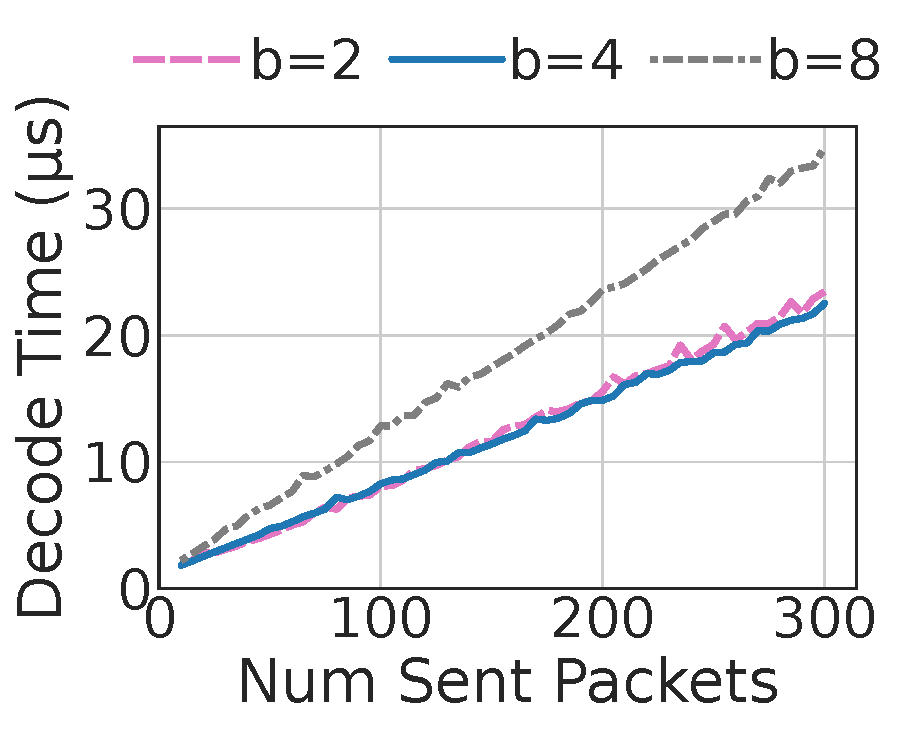
\includegraphics[width=\linewidth,trim={3mm 0 7mm 0},clip]{quack/figures/fig2a_quack_num_candidates_vs_decode_time.pdf}
	\caption{Evaluate a degree-$m=t=10$ polynomial at $n$ candidate roots.}
	\label{fig:quack:psum:n-vs-decoding}
\end{subfigure}
\hspace{-0.1em}
\begin{subfigure}{0.32\columnwidth}
	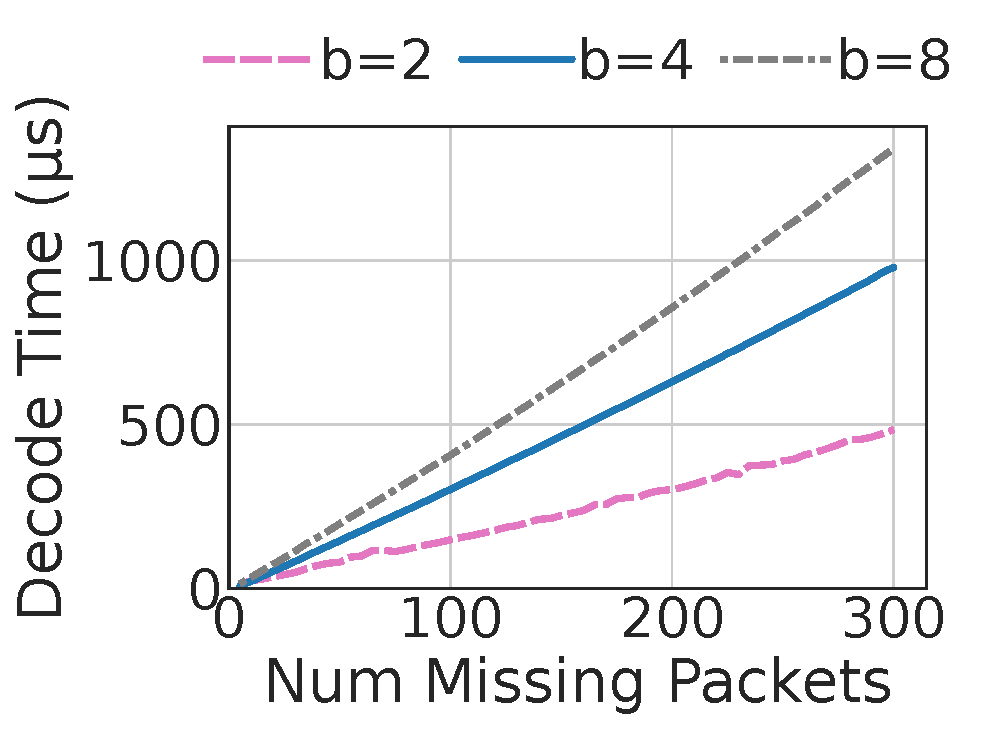
\includegraphics[width=\linewidth,trim={3mm 0 7mm 0},clip]{quack/figures/fig2b_quack_num_missing_vs_decode_time.pdf}
	\caption{Plug $n=300$ candidate roots into a degree-$m$ polynomial.}
	\label{fig:quack:psum:m-vs-decoding}
\end{subfigure}
\hspace{-0.1em}
\begin{subfigure}{0.32\columnwidth}
	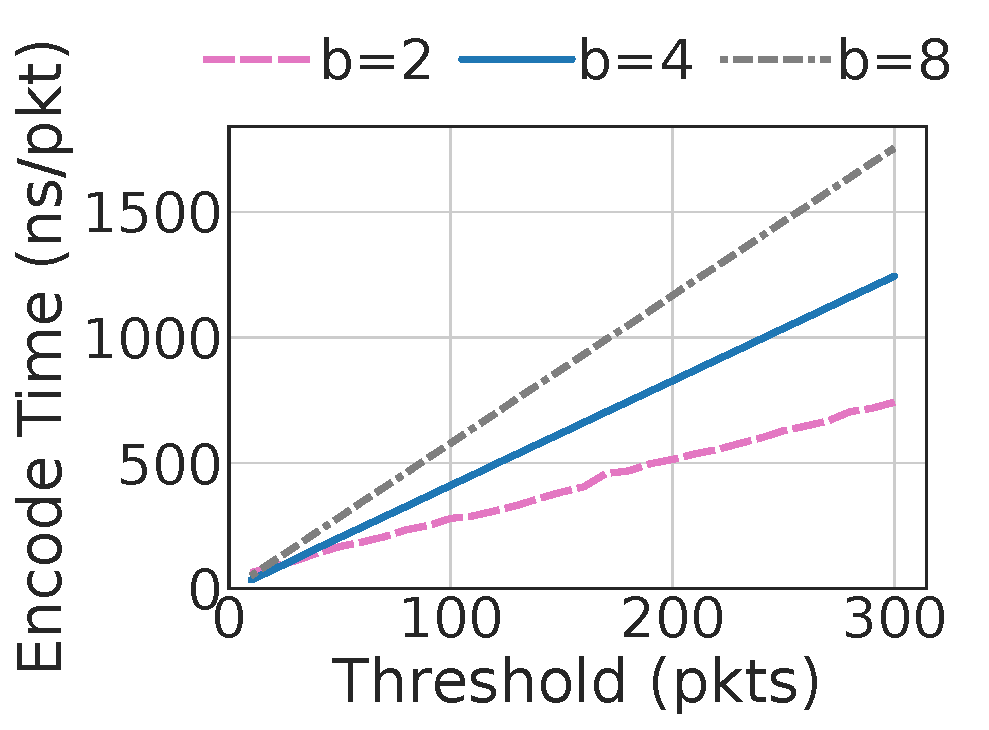
\includegraphics[width=\linewidth,trim={3mm 0 7mm 0},clip]{quack/figures/fig2c_quack_threshold_vs_encode_time.pdf}
	\caption{Update $t$ power sum equations.
	Average of $1000$ packets.}
	\label{fig:quack:psum:construction-time}
\end{subfigure}
\caption{How power sum quACK performance depends on various parameters:
bit width, threshold, number of sent and missing packets.
Average of 100 trials.
}
\label{fig:quack:psum}
\end{figure}


In this section, we benchmark the power sum quACK construction and evaluate the
computation cost for different parameters in packet-scale settings.
We explore different bit widths for the identifier and settle on
using 32-bit packet identifiers.
Our microbenchmarks used an m4.xlarge AWS instance with a 4-CPU Intel Xeon E5
processor @ 2.30 GHz and 16 GB memory.

\subsection{Identifier bit widths}
\label{sec:quack:psum-microbenchmarks:bit-widths}

The more bits we use in an identifier, the less likely that there will be a
collision, but different bit widths have different implications for the
computation cost based on which instructions the CPU can use. Modular
operations are efficient for 16- and 32-bit integers, fitting within the 64-bit
word size (the number of bits that can be processed in one instruction) of most
modern CPUs. For example, to multiply two 32-bit integers, we cast them to
64-bit integers, multiply, then take the modulus.

\Cref{fig:quack:psum} shows the best encoding and decoding times we achieved
at different bit widths, demonstrating that computation cost is generally higher
for higher bit widths, though not significantly. For 16-bit identifiers only, we
precomputed power tables that fit in the L3 cache. For 64-bit identifiers, we
implemented Montgomery modular multiplication~\cite{montgomery1985modular}
to avoid an expensive hardware division for 128-bit integers. In the remainder
of this dissertation, we select $b=4$, or 32-bit identifiers, as the preferred
tradeoff between collision probability, the size of the quACK, and computation
cost.

\subsection{Encoding time}
\label{sec:quack:psum-microbenchmarks:encoding}

Encoding a single packet requires updating the $t$ power sums in the power sum
quACK.
The per-packet encoding time is thus directly proportional to the threshold
number of missing packets $t$ (\Cref{fig:quack:psum:construction-time}) at
$\approx 3$ ns/power sum.
Each power sum can be updated in a constant number of operations based on the
previous power sum, which is a single modular addition and multiplication.

\subsection{Decoding time}
\label{sec:quack:psum-microbenchmarks:decoding}

Decoding the power sum quACK requires finding the solution to a system of power
sum polynomial equations. This boils down to applying Newton's identities (a
linear algorithm) and finding the roots of a polynomial equation in a modular
field~\cite{eppstein2011straggler}.
Factoring a polynomial is asymptotically fast in theory, but the implementation
is branch-heavy and complicated~\cite{batut2000user}.
We find that in practice, it is faster to plug in and determine which of the
$n$ candidate roots evaluate to zero when there are $n < 40,000$ roots.
We use this method to decode the power sum quACK instead of factorization.

The decoding time of this method is directly proportional to the number of
candidate packets $n$ (\Cref{fig:quack:psum:n-vs-decoding})
and the number of missing packets $m$ (\Cref{fig:quack:psum:m-vs-decoding}).
Decoding takes $\approx 11$ ns/candidate/missing, and both $n$ and $m$ are
typically a few hundred at most.
Thus it is typically for encoding to take a few nanoseconds per packet and
decoding to take a few microseconds per quACK.

\section{IBLT microbenchmarks}
\label{sec:quack:iblt-microbenchmarks}

Both constructions of the quACK implement the same interface and can be used
interchangeably, so when should we prefer one to the other? In this section, we
compare the encoding and decoding times of each construction in practice,
including how they scale with the communication cost and the number of missing
packets. We also explore how to configure the IBLT quACK based on its
probabilistic correctness. We run the microbenchmarks on a single core of an
AWS m4.xlarge instance.

\subsection{Encoding and decoding time scalability}
\label{sec:quack:iblt-microbenchmarks:scalability}

\begin{figure}[t]
    \centering
    \begin{subfigure}[b]{0.37\linewidth}
        \centering
        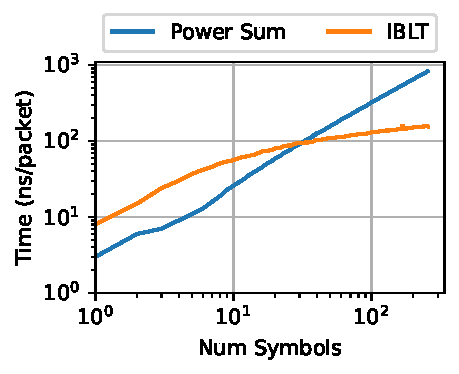
\includegraphics[width=\linewidth]{quack/figures/quack_encode.pdf}
        \caption{Encode time.}
        \label{fig:quack:iblt-computation:encode}
    \end{subfigure}
    \begin{subfigure}[b]{0.37\linewidth}
        \centering
        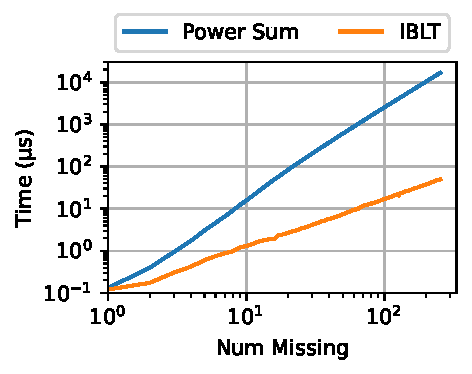
\includegraphics[width=\linewidth]{quack/figures/quack_decode.pdf}
        \caption{Decode time.}
        \label{fig:quack:iblt-computation:decode}
    \end{subfigure}
    \caption{IBLT vs. power sum quACK microbenchmarks. The IBLT quACK is more
     computationally scalable than the power sum quACK, but the encoding time
     suffers from constant factor overheads with a smaller number of symbols.
     The cumulative time of the trials is at least $100$ ms.
     }
    \label{fig:quack:iblt-computation}
\end{figure}

Encoding and decoding operations in the IBLT quACK update a logarithmic number
of symbols per-packet, compared to all of the symbols in the power sum quACK.
This results in better computational complexity in theory, but in practice we
find that the encoding and decoding times also depend on the constant factor
overheads of the pseudorandom mapping algorithm.

The encoding time in the IBLT quACK is faster when there are at least
$\approx\!30$ symbols (\Cref{fig:quack:iblt-computation:encode}).
Each update in the IBLT uses an expensive square root instruction in the
pseudorandom mapping algorithm, adding constant factor overheads that impact
smaller numbers of symbols.

The decoding time is faster for any number of symbols
(\Cref{fig:quack:iblt-computation:decode}).
Note that the power sum quACK actually uses a decoding method that is linear
in \textit{all} packets received, not just the \textit{missing} packets, due to
the complexity of symmetric polynomial factorization.

\subsection{Probabilistic correctness}
\label{sec:quack:iblt-microbenchmarks:correctness}

\begin{figure}[t]
    \centering
    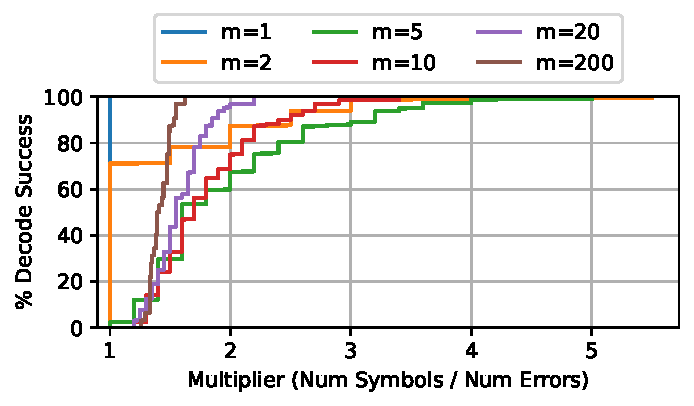
\includegraphics[width=0.9\linewidth]{quack/figures/quack_multiplier.pdf}
    \caption{The CDF of the minimum number of symbols $t$ needed to successfully
    decode an quACK for various numbers of missing packets $m$, 100000 trials.}
    \label{fig:quack:iblt-correctness}
\end{figure}

It is unknown how many symbols are required in the IBLT quACK to decode the same
number of $m$ missing packets using power sums in the previous benchmarks.
There is a constant multiplicative factor on average
($1.23$--$1.35\times$~\cite{yang2024practical,baek2023simple}), but this is
not necessarily representative when $m$ is often small.
\Cref{fig:quack:iblt-correctness} shows the CDF of the minimum number of symbols
to decode various $m$ as this constant multiplier increases. $m=1$ trivially
requires one symbol, while the multiplier decreases for higher $m$ to achieve
the same success rates.

The sender does not know how many symbols it needs to encode to later decode a
certain $m$. Using the power sum quACK, this is exactly $m$ symbols. In the
IBLT quACK, $4 \cdot m$ symbols have at least a $\!98.8\%$ success rate for all
$m$ evaluated in \Cref{fig:quack:iblt-correctness}. When $m$ is large, the IBLT
quACK utilizes more of the link than the power sum quACK, but maintaining more
symbols at the sender and receiver means the sender has a greater worst-case
tolerance for errors with more scalable encoding overheads.

\section{Summary}
\label{sec:quack:summary}

\begin{table*}[ht]
  \centering

  \begin{subtable}[b]{\linewidth}
  \centering
  \begin{tabular}{lccc}
    \toprule
    & \bf Encode Time & \bf Decode Time & \bf QuACK Size \\
    \midrule
    Strawman 1a & $O(1)$ & $O(1)$ & \textcolor{red}{$O(n)$} \\
    Strawman 1b & $O(1)$ & $O(1)$ & \textcolor{red}{$O(n)$} \\
    Strawman 1c & $O(1)$ & $O(1)$ & \textcolor{red}{$O(n)$} \\
    Strawman 2 & $O(1)$ & \textcolor{red}{$O(\binom{n}{t})$} & $O(1)$ \\
    \bf \textcolor{black!50!blue}{Power Sums} & \bf \textcolor{black!50!blue}{$O(t)$} & \bf \textcolor{black!50!blue}{$O(t^2)$} & \bf \textcolor{black!50!blue}{$O(t)$} \\
    \bf \textcolor{black!50!blue}{IBLT} & \bf \textcolor{black!50!blue}{$O(\log t)$} & \bf \textcolor{black!50!blue}{$O(t\log t)$} & \bf \textcolor{black!50!blue}{$O(t)$} \\
    \bottomrule
  \end{tabular}
  \caption{The algorithmic complexity of the costs of each quACK construction.
  $n = |S|$ is the total number of sent elements, $t \geq |S \setminus R|$ is an
  upper bound on the number of missing elements.\\
  }
  \label{tab:quack:overview:theoretical}
  \end{subtable}

  \begin{subtable}[b]{\linewidth}
  \centering
  \begin{tabular}{lcccccc}
    \toprule
    & \bf Encode & \bf Decode & \bf Num & \bf Num & \bf  & \bf Cumu- \\
    & \bf Time & \bf Time & \bf Packets & \bf Bytes & \bf Protocol & \bf lative? \\
    \midrule
    Strawman 1a & N/A & N/A & \textcolor{red}{$500$} & $4$ & UDP & No \\
    Strawman 1b & N/A & N/A & \textcolor{red}{$500$} & $4 \cdot window$ & UDP & No \\
    Strawman 1c & N/A & N/A & \textcolor{red}{$\geq 500$} & $4$ & \textcolor{red}{TCP} & Yes \\
    Strawman 2 & $27$ ns/pkt & \textcolor{red}{$88$ Myears} & $1$ & $36$ & UDP & Yes \\
    \bf \textcolor{black!50!blue}{Power Sums} & \bf \textcolor{black!50!blue}{$26$ ns/pkt} & \bf \textcolor{black!50!blue}{$15.5$ $\mu$s} & \bf \textcolor{black!50!blue}{$1$} & \bf \textcolor{black!50!blue}{$48$} & \bf \textcolor{black!50!blue}{UDP} & \bf \textcolor{black!50!blue}{Yes} \\
    \bf \textcolor{black!50!blue}{IBLT} & \bf \textcolor{black!50!blue}{$42$ ns/pkt} & \bf \textcolor{black!50!blue}{$1.3$ $\mu$s} & \bf \textcolor{black!50!blue}{$1$} & \bf \textcolor{black!50!blue}{$\geq 58$} & \bf \textcolor{black!50!blue}{UDP} & \bf \textcolor{black!50!blue}{Yes} \\
    \bottomrule
  \end{tabular}
  \caption{A concrete realization of the costs of each quACK construction.
  Parameters: $n=500$, $t=10$, and the elements are 32-bit integers.}
  \label{tab:quack:overview:practical}
  \end{subtable}

  \caption{ The computation and communication costs of the power sum and IBLT
  quACK constructions are comparable to or better than those of the strawmen.
  The encoding time includes inserting an element into the data structure that
  represents the quACK(s). The decoding time
   includes finding the elements of either $S \setminus R$ or $R \subseteq S$,
   given the quACK(s) and $S$.}
  \label{tab:quack:overview}
\end{table*}


The power sum and IBLT constructions of the quACK can efficiently refer to and
acknowledge a set of randomly encrypted packets
(\Cref{tab:quack:overview:practical}). These constructions are efficient to
decode, add reasonable link overhead, and are cumulative representations of the
packets seen by the receiver. Compared to Strawman 2, the quACKs can be decoded
with simple computational primitives such as XORs and modular arithmetic. Their
link overheads are proportional only to the number of missing packets between
consecutive quACKs, up to a configurable threshold. In comparison, the link
overhead of Strawman 1 is necessarily proportional to the number of received
packets. Our quACK constructions are also resilient to mis-identifying a
received packet as dropped, in the case a quACK is lost in transmission.

Compared to each other, the IBLT quACK has more scalable computational costs
than the power sum quACK but greater constant factor overheads
(\Cref{tab:quack:overview:theoretical}). We find the IBLT quACK to be more
useful when a large number of symbols is required, such as in settings with
high, bursty loss. However, the power sum quACK is still more efficient when
loss is small or infrequent. In addition, since the power sum quACK is
deterministically correct, it may be simpler to reason about when the threshold
is predictable. Thus both constructions have different tradeoffs to consider.

\section{Appendix: Optimizing the power sum quACK at various bit widths}
\label{sec:quack:appendix}

\begin{table}[ht]
  \centering
  % \renewcommand{\arraystretch}{0.000023}
  \begin{tabular}{lcccrrr}
    \toprule
    \bf     & \bf        & \bf       & \bf        & \bf Per-Packet & \bf Decode & \bf Size\\
    \bf Bits  & \bf NF     & \bf PC    & \bf MM     & \bf Encode Time & \bf Time     & \bf (bytes)\\
    \midrule
    32     &        &       &        & $149$ ns & $3.18$ ms      & 82 \\
    \bf \textcolor{black!50!blue}{32*} & \bf \textcolor{black!50!blue}{x} & & & \bf \textcolor{black!50!blue}{151 ns} & \bf \textcolor{black!50!blue}{102 ${\mu}$s} & \bf \textcolor{black!50!blue}{82} \\
    32     & x      &       & x      & $163$ ns & $130$ ${\mu}$s & 82 \\
    16     & x      &       &        & $137$ ns & $101$ ${\mu}$s & 42 \\
    16*    & x      & x     &        & $57$ ns & $43$ ${\mu}$s & 42 \\
    16     & x      & x     & x      & $84$ ns & $48$ ${\mu}$s & 42 \\
    63     & x      &       &        & $1.14$ ${\mu}$s & $622$ ${\mu}$s & 162 \\
    63*    & x      &       & x      & $159$ ns & $121$ ${\mu}$s & 162 \\
  % 64*    & x      &       & x      & $177$ ns & $132$ ${\mu}$s & 162 \\
    \bottomrule
    % removed factoring except for base 32 case since typically faster
    % removed power table for 64 bit because too large
    % removed both power table + montgomery for 16/32 bit to not combine opts
    % * represents optimal for that bit width
  \end{tabular}
  \caption{Power sum QuACK with different bit widths and optimizations,
  using $n=1000$, $t=20$. The three optimizations are not factoring (NF),
  pre-computation (PC), and Montgomery multiplication (MM).
  *Recommended optimizations for that bit width.}
  \label{tab:optimized-quack}
\end{table}


\chapter[Sidekick Protocols]{Sidekick Protocols: Secure in-network assistance for data senders}
\label{sec:sidekick}

This chapter describes \emph{Sidekick protocols}: an approach to in-network
assistance for secure transport protocols. In this approach, in-network
intermediaries help endpoints by sending information adjacent to the underlying
connection, which remains opaque and unmodified on the wire. Described in \Cref
{sec:quack}, this information is called a quACK, and the quACK is the key
technical tool that allows proxies to usefully refer to a set of packets that
they have received even when the transport headers are randomly encrypted. In
real-world and emulation-based evaluations, the Sidekick protocol improves
performance in several scenarios: early retransmission over lossy Wi-Fi paths,
proxy acknowledgments to save energy, and a path-aware congestion-control
mechanism we call \emph{PACUBIC}. The path-aware CUBIC congestion control
algorithm emulates the congestion response of a ``split'' connection from the
perspective of the data sender at the endpoint, without buffering packets at
the proxy.

\section{Introduction}
\label{sec:sidekick:intro}

In the Internet's canonical model, transport is end-to-end and implemented only
in hosts. Traditionally, routers and other network components forwarded IP
datagrams without regard to their payloads or flow membership~\cite
{saltzer1984endtoend, clark1988darpa}; only hosts thought about connections,
reliable delivery, or flow-by-flow congestion control.

In practice, however, the best behavior for a transport protocol depends on the
particulars of the network path. An appropriate retransmission or
congestion-control scheme for a heavily-multiplexed wired network wouldn't be
ideal for paths that include a high-delay satellite link, Wi-Fi with bulk ACKs
and frequent reordering, or a cellular WWAN~\cite
{kuhn2021quic-over-sat,goyal2017abc}.

By the 1990s, many networks had broken from the canonical model by deploying
in-network TCP accelerators, also known as ``performance-enhancing proxies''
(PEPs)~\cite{rfc3135}. TCP PEPs can split an end-to-end connection into
multiple concatenated connections~\cite
{kapoor2005achieving,caini2006pepsal,davern2011httpep,farkas2012splittcp,hayes2019mmwave},
buffer and retransmit packets over a lossy link~\cite
{balakrishnan1995snoop,polese2017milliproxy}, virtualize congestion
control~\cite{cronkite2016vcc,he2016acdc,mihaly2012mobilePEP}, resegment the
byte stream, and enable forward error correction, explicit congestion
notification, or other segment-specific enhancements. Because TCP isn't
encrypted or authenticated, PEPs can achieve this transparently, without the
knowledge or cooperation of end hosts. Roughly 20--40\% of Internet paths cross
at least one TCP PEP~\cite{imc2011handley, edeline2019bottomup}.

While many flows benefit from PEPs, their use carries a cost: protocol
ossification~\cite{papastergiou2017deossifying, edeline2019bottomup}. When a
middlebox inserts itself in a connection and enforces its preconceptions about
the transport protocol, it can thwart the protocol's evolution, dropping
traffic that uses an upgraded version or new options. TCP PEPs have hindered or
complicated the deployment of many TCP improvements, such as ECN++, tcpcrypt,
TCP extended options, and multipath TCP~\cite
{mandalari2018ecnplusplus,imc2011handley,raiciu2012multipathtcp}.

In response to this ossification, and to an increased emphasis on privacy and
security, post-TCP transport protocols have been designed to be impervious to
meddling middleboxes, by encrypting and authenticating the transport header. We
refer to these newer transport protocols as ``secure'' transport protocols. The
most prevalent is QUIC~\cite{rfc9000}, found in billions of installed Web
browsers and millions of servers~\cite{zirngibl2021quicdeployment}; other secure
transport protocols are used in WebRTC/SRTP~\cite{rfc8834webrtc},
Zoom~\cite{zoom}, BitTorrent~\cite{bittorrent}, and
Mosh/SSP~\cite{winstein2012mosh}.

This encryption means that middleboxes can't interpose themselves on a
connection or understand the sequence numbers of packets in transit. This
prevents PEPs from providing assistance, reducing---in some situations---the
performance of secure transport protocols~\cite
{border2020quicsat-presentation,kuhn2021quic-over-sat,martin2022bbr-quic-sat,border2020evaluating,kosek2022quicpep}.
It's possible to co-design protocols and PEPs to preserve security and privacy
while permitting assistance from credentialed middleboxes~\cite
{ford2008logjam,sherry2015blindbox, dogar2012tapa,iyengar2009flow}, but
challenging to do so without tightly coupling these components, risking
ossification and fragility.

In this chapter, we propose a method for in-network assistance of secure transport
protocols that tries to resolve this tension. Our approach leaves the transport
protocol unchanged on the wire: an encrypted end-to-end connection between hosts,
opaque to middleboxes and free to evolve. No PEPs are credentialed to decrypt
the transport protocol's headers.

Instead, we propose a second protocol to be spoken on an adjacent connection
between an end host and a PEP. We call this the \emph{\bf Sidekick protocol},
and its contents are \emph{about} the packets of the underlying, or ``base,''
connection. Sidekick PEPs assist end hosts by reporting what they've observed
about the packets of the encrypted base connection, without coupling their
assistance to the details of the base protocol. End hosts use this information
to influence decisions about how and when to send or resend packets on the base
connection, approximating some of the performance benefits of traditional PEPs.
We first proposed a similar functional separation in \cite{yuan2022sidecar},
and presented a concrete realization of the idea and its nuanced
interactions with real transport protocols in \cite{yuan2024sidekick}.

One key technical challenge with this approach is how the Sidekick can
efficiently refer to ranges of packets in an encrypted base connection. These
packets appear random to the middlebox, and referring to a range of, e.g., 100
encrypted packets in the presence of loss and reordering is not as simple as
saying ``up to 100'' when there are cleartext sequence numbers. In \Cref
{sec:quack}, we presented and evaluated a mathematical tool called a \emph
{\bf quACK} that concisely represents a selective acknowledgment of randomly
encrypted packets. In this chapter, we leverage the power sum quACK,
based on the insight that we can model the problem as a system of power
sum polynomial equations if there is a practical bound on the maximum number of
``holes'' among the packets being ACKed.

A second challenge is how the end host should use information from a Sidekick
connection to obtain a performance benefit for its base connection. Since the
performance benefit comes from changing behavior at the end host rather than
the middlebox, transport protocols need to incorporate this information into
their existing algorithms for, e.g., loss detection and retransmission, which
have gotten increasingly complex over time. To explore this, we designed a
Sidekick protocol and integrated it into client implementations in three scenarios:
\begin{itemize}[noitemsep,topsep=2pt]
\item A low-latency audio stream over an Internet path that includes a Wi-Fi path segment
  (low latency with loss), followed by a WAN path segment (higher latency
  with low loss). Can the Sidekick PEP reduce the de-jitter buffer delay
  by triggering earlier retransmissions on loss?

\item An upload over the same path. Can a secure transport protocol like QUIC,
  aided by a Sidekick PEP at the point between these two path segments, match
  the throughput of TCP over a connection-splitting PEP?

\item A battery-powered receiver, downloading data from the Internet over Wi-Fi.
  If the Wi-Fi access point sends Sidekick quACKs on behalf of the receiver,
  can it reduce the number of times the receiver's radio needs to wake up
  to send an end-to-end ACK?
\end{itemize}

\smallskip

A third technical challenge is how knowledge about \emph{where}
loss occurs along a path should influence a congestion-control scheme.
The challenge in any such scheme is how to maximize the congestion window
while sharing the network fairly with competing flows.
We present a path-aware modification to the CUBIC congestion-control
algorithm~\cite{ha2008cubic}, which we call \mbox{\textbf{PACUBIC}},
that approximates the congestion-control behavior of a PEP-assisted split TCP
CUBIC connection while making its decisions entirely on the host.

\paragraph{Summary of results.}

We implemented the Sidekick protocol in a low-latency media client
based on the WebRTC standard, and an HTTP/3 client using the Cloudflare
implementation of QUIC~\cite{quiche} and the \texttt{libcurl}~\cite{libcurl}
implementation of HTTP/3. We evaluated the three scenarios in
real-world and emulation experiments.
In real-world experiments using an unmodified local Wi-Fi network to access our
nearest AWS datacenter, the Sidekick was able to trigger early retransmissions
to fill in gaps in the audio of a latency-sensitive audio stream, reducing the
receiver's de-jitter delay from 2.3~seconds to 204~ms---about a 91\% reduction
(\Cref{fig:real-world}). The Sidekick was also able to improve the speed of an
HTTP/3 (QUIC) upload by about 50\%.

In emulation experiments of the ``battery-powered receiver'' scenario,
the Sidekick PEP was able to reduce the need for the receiver to send ACKs
by sending proxy acknowledgments on its behalf---ACKs the sender used
to advance its flow-control and congestion-control windows. The
receiver only needed to wake up its radio to send occasional
end-to-end ACKs, which the sender used to discard data from its
buffer (\Cref{fig:ack-reduction}).

Also in an emulation experiment, we confirmed that PACUBIC's
performance approximates a split CUBIC connection (two TCP CUBIC
connections separated by a PEP), responding to loss events on the
different path segments similarly to how the individual CUBIC flows would
(\Cref{fig:loss-vs-tput}). The results indicate that the Sidekick protocol's gains
do not come at the
expense of congestion-control fairness relative to a split CUBIC connection.

\smallskip

The rest of this chapter discusses three motivating scenarios for the Sidekick
(\Cref{sec:sidekick:motivating}), describes the concrete Sidekick protocol we
built around power sum quACKs (\Cref{sec:sidekick:init,sec:sidekick:sender}) and
its implementation in two base protocols (\Cref{sec:sidekick:implementation}),
and then evaluates the protocol in real-world (\Cref{sec:sidekick:real-world})
and emulation experiments (\Cref{sec:sidekick:emulation}).

\section{Motivating scenarios}
\label{sec:sidekick:motivating}

\begin{figure}[t]
	\centering
	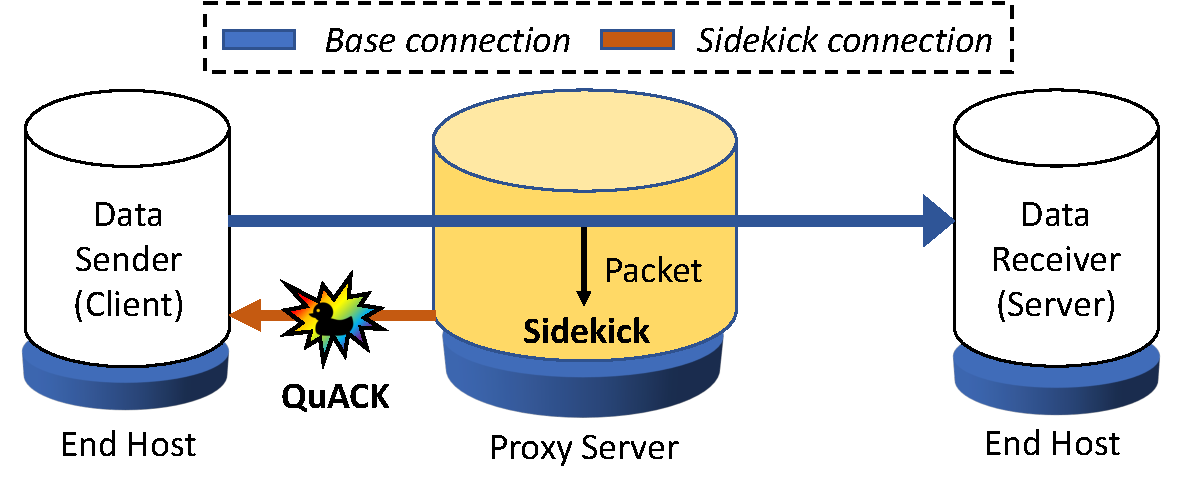
\includegraphics[width=0.8\linewidth]{sidekick/figures/sc_protocol.pdf}
\caption{The proxy generates quACKs, in-network acknowledgments, based on
the encrypted packets it observes in the base protocol. It quACKs to an end
host, the data sender, which sends or resends packets on the base protocol as a result.
Although we only show one side of the connection, the Sidekick could assist
either end host of a bidirectional flow.
}
\label{fig:sidekick:overview}
\end{figure}


We focus on three scenarios where end hosts benefit from in-network assistance.
In each one, a proxy provides feedback in the form of a quACK to an end
host: the data sender (\Cref{fig:sidekick:overview}). Recall that a quACK is a
``cumulative ACK + selective ACK'' over encrypted packet identifiers. The data
sender uses this feedback to influence its behavior on the base connection,
without altering the wire format.

To be clear: the Sidekick protocol is not tied to a specific base protocol
nor to how the end hosts use the quACK information. The base protocol does not
need to be reliable, nor to have unique datagrams---we implemented and evaluated
the same Sidekick protocol and the same proxy behavior across the different
scenarios in this paper.

\subsection{Low-latency media retransmissions}
\label{sec:sidekick:motivating:media}

Consider a train passenger using on-board Wi-Fi to have a low-latency audio
conversation, using WebRTC/SRTP~\cite{rfc8834webrtc}, with a friend. The
end-to-end network path contains a low-latency, high-loss ``near'' path
segment (the Wi-Fi hop) followed by a high-latency, low-loss ``far'' path
segment (the cellular and wired path over the Internet). The friend probably
suffers from poor connection quality, experiencing drops in the audio stream or
high de-jitter buffer delays from waiting for retransmitted packets to be
played in order (\Cref{fig:sidekick:real-world:media} in the real world,
\Cref{fig:sidekick:main-results:media} in emulation).

In the Sidekick approach, a PEP on the Wi-Fi access point sends quACKs to
the media client on the passenger's laptop, assisting the base connection.
The passenger's media client uses quACKs to retransmit packets sooner than they
would have using negative acknowledgments (NACKs) from the friend. The
end result is similar to the effect of PEPs such as
Snoop~\cite{balakrishnan1995snoop} and Milliproxy~\cite{polese2017milliproxy}
that leverage TCP's cleartext sequence numbers to trigger early retransmission
on lossy wireless paths.

\subsection{Emulating split congestion control in an HTTP/3 file upload}
\label{sec:sidekick:motivating:http}

Consider the same train passenger as before but uploading a large file over the
Internet with a reliable transport protocol. If the protocol were TCP, the
train could deploy a split TCP PEP at the access point. The split connection
allows quick detection and retransmission of dropped packets on the lossy Wi-Fi
segment, while opening up the congestion window on the high-latency cellular
segment.

However, secure transport protocols like QUIC can't benefit from (nor be harmed
by) connection-splitting PEPs. Without a PEP, QUIC relies on end-to-end
mechanisms over the entire path to detect losses, recover from them, and adjust
the congestion-control behavior. This leads to reduced upload speeds
(\Cref{fig:sidekick:real-world:pep-emulation} in the real world,
\Cref{fig:sidekick:main-results:pep-emulation} in emulation).

With help from the same Sidekick PEP, the QUIC client combines information from
quACKs and end-to-end ACKs to emulate the congestion-control behavior of a
split TCP connection (\Cref{sec:sidekick:pacubic}). The
application considers whether packets are lost on the near or far path
segments, and adjusts the congestion window accordingly while respecting the
opacity of the end-to-end base connection. The application also retransmits the
packet as soon as the loss has been detected.

The only guarantee the proxy makes to the client via the quACK is that it has
received some packets. To respect the end-to-end reliability contract with the
server, the client does not delete packets that may need to be transmitted
until it receives an end-to-end ACK from the server, even if the packet has
been quACKed by the proxy.

\subsection{Battery-saving ACK reduction}
\label{sec:sidekick:motivating:ack-reduction}

Now consider a battery-powered device downloading a large file from the
Internet. To reduce how often the device's
radio needs to wake up, saving energy, the base connection can reduce the
frequency of end-to-end ACKs the device sends to the data sender.
ACK reduction has also been shown to improve performance by reducing collisions
and contention over half-duplex links~\cite{custura2023reducing,li2020tack}.
The ACK frequency can be configured with a TCP kernel setting or proposed
QUIC extension~\cite{ietf-quic-ack-frequency-07}.

However, ACK reduction can also degrade
throughput~\cite{custura2023reducing,custura2020impact}
(\Cref{fig:sidekick:main-results:ack-reduction} in emulation).
The data sender receives more delayed feedback about loss, and has to carefully
pace packets to avoid bursts in the large delay between ACKs.
One proposal has the PEP acknowledge packets on behalf of the data
receiver~\cite{kliazovich2012arqproxy}, leveraging cleartext TCP sequence
numbers. This proposal does not apply to secure transport protocols without
these sequence numbers.

In this scenario, a Sidekick proxy at a Wi-Fi access point or cellular base station
quACKs to the data sender on behalf of the battery-powered device. The device still occasionally
wakes up its radio to send ACKs, but the data sender uses the more frequent quACKs
from the proxy to advance its flow-control and congestion-control windows.

The data sender respects the end-to-end reliability contract by only deleting packets
in response to end-to-end ACKs, but disregards the data receiver's flow control by using quACKs
to advance the flow-control window. If the data sender only used end-to-end ACKs to advance the
window, it would waste time waiting between ACKs to send packets with too small
a window, and need to pace sent packets on receiving a large ACK with too large
a window.

\section{Design}
\label{sec:sidekick:design}

This section describes our design for a Sidekick protocol built around
quACKs. This includes the setup and configuration of a Sidekick
connection, how a sender detects loss from a quACK, and a path-aware
modification to CUBIC called PACUBIC, for congestion-controlled base
protocols.

%%%%%%%%%%%%%%%%%%%%%%%%%%%%%%%%%%%%%%%%%%%%%%%%%%%%%%%%%%%%%%%%%%%%%%%%%%%%%%%

\subsection{PEP discovery mechanism}
\label{sec:sidekick:design:discovery}

% In most settings, such as 4G/5G cellular networks,
PEPs have traditionally been deployed as transparent proxies, silently
interposing on end-to-end connections. Senders therefore need a way to detect
transparent Sidekick proxies and inform them of where to send quACKs.  Because
of network address translation, all communication to the proxy must be
initiated by the sender or use the same IP addresses and port numbers of the
base connection.

Our design has senders signal quACK support by sending a
distinguished packet containing a 128-byte \emph{sidekick-request} marker.
Such inline signaling could confuse receivers, but Sidekicks target protocols
such as QUIC that discard cryptographically unauthenticated data anyway.  It
would be cleaner to signal support through out-of-band UDP options~\cite
{ietf-tsvwg-udp-options-28}, which we may hope to do once standardized.
The proxy replies to a sidekick-request packet by sending a special packet from
the receiver's IP address and port number back to the sender. This packet
contains a \emph{sidekick-reply} marker, an opaque session ID, and an IP
address and port number for communicating with the proxy.

% Sidekick connections can be configured explicitly or implicitly.
In systems that explicitly configure proxies, such as Apple's iCloud Private
Relay~\cite{icloud-private-relay} based on MASQUE~\cite
{kosek2021masque,kramer2021masquepep}, proxies can simply negotiate sending
quACKs during session establishment. However, any explicit proxy configuration
has the disadvantage that the proxy may not be on the most direct network path.
Explicit proxies also make mobility and handoffs more challenging.

\subsubsection{Security.}
A malicious third-party could execute a reflection amplification attack that
generates a large amount of traffic while hiding its source. This is
possible because the sender requests quACKs to a different port and (for some
carrier-grade NATs) IP address from the underlying session. To mitigate this,
each quACK can contain a quota, initially 1, of remaining quACKs the proxy
will send as well as an updated session ID\@.
The quota and session ID ensure only the sender can increase the quota or
otherwise reconfigure the session.

An adversarial PEP could send misleading information to the sender. Note that
only on-path PEPs can send credible information, since they refer to unique
packet identifiers.
To mitigate this, the sender can consider PEP feedback along with
end-to-end metrics to determine whether to keep using the PEP. The sender can
always opt out of the PEP, and the PEP cannot actively manipulate traffic any
more than outside a Sidekick setting.

%%%%%%%%%%%%%%%%%%%%%%%%%%%%%%%%%%%%%%%%%%%%%%%%%%%%%%%%%%%%%%%%%%%%%%%%%%%%%%%

% \subsection{Handshake}
% \label{sec:sidekick:design:handshake}

% Upon receiving the sidekick-reply packet, the sender begins communicating
% directly with the proxy from a different UDP port.  It initially sends
% back the session ID and configuration parameters to start receiving
% quACKs.

\subsection{Sidekick protocol messages}

\begin{figure}[t]
    % \centering
    % Client payloads
    \begin{subfigure}[b]{0.48\linewidth}
        \begin{protopayload}{\texttt{Init}}
            \begin{lstlisting}[language=Rust]
epoch: u32;
base_conn: [u8; 12];
quack_ty: u8;
num_symbols: u8;
id_offset: u16;
quack_pkts: u16;
quack_ms: u16;
            \end{lstlisting}
        \end{protopayload}
        \begin{protopayload}{\texttt{Reset}}
            \begin{lstlisting}[language=Rust]
epoch: u32;
errno: u32;
            \end{lstlisting}
        \end{protopayload}
        \caption{Client payloads.}
        \label{fig:sidekick:payloads:client}
    \end{subfigure}
    \hfill
    % Proxy payloads
    \begin{subfigure}[b]{0.48\linewidth}
        \begin{protopayload}{\texttt{InitACK}}
            \begin{lstlisting}[language=Rust]
epoch: u32;
udp_port: u16;
errno: u32;
            \end{lstlisting}
        \end{protopayload}
        \begin{protopayload}{\texttt{QuACK}}
            \begin{lstlisting}[language=Rust]
count: u32;
last_element: u32;
code: Vec<Symbol>;
            \end{lstlisting}
        \end{protopayload}
        \caption{Proxy payloads.}
        \label{fig:sidekick:payloads:proxy}
    \end{subfigure}
  % Caption
  \caption{Sidekick protocol messages to configure and reset the Sidekick
  connection.}
  \label{fig:sidekick:payloads}
\end{figure}


Once the client has an IP address and port for communicating with the proxy, it
can establish an adjacent Sidekick connection with the proxy from a different
local UDP port. The client can then send various messages to the proxy to
configure the connection and reset bad state, while receiving quACKs to decode
and adjust the behavior of the base connection (\Cref{fig:sidekick:payloads}).

\subsubsection{Configuration.}
In the \texttt{Init} message, the sender configures (i) which quACK construction
to use and the number of symbols, (ii) a byte offset into the packet payload at
which to compute the 4-byte identifier, and (iii) the interval at which the PEP
should send quACKs.
The proxy accepts or rejects these configurations with an \texttt{InitACK}
and, if accepted, immediately begins to send \texttt{QuACK} messages.

The number of symbols represents the upper bound on the number of missing
packets between quACKs, in practice the number of ``holes'' among the packets
that are selectively ACKed. This bound depends on the quACK interval, and
should be set based on how precise loss detection needs to be and other
qualities of the link. For example, the number of symbols should be larger to
detect congestive loss in the queue of a bottleneck link, or smaller to detect
transmission error on a lossy link.

The quACK interval is expressed in terms of time or number of packets,
 e.g., every $N$ milliseconds or every $N$ packets, as in a TCP delayed ACK.
The sender determines the desired interval based on its estimated
RTT of the base connection and its application objectives, e.g.,
more frequently for latency-sensitive applications or lower-RTT paths.

\subsubsection{Resets.}
The Sidekick protocol allows the sender to tell the PEP to reinitialize the
quACK. The \texttt{Reset} message acts as a synchronization point in the base
connection in which both the client and proxy disregard old packets and start
a new cumulative quACK. This is helpful if the quACK becomes invalid, e.g.,
if the number of missing packets exceeds the maximum bound. It is always safe
to reset the quACK, or even to ignore the Sidekick entirely and fall back to the
base protocol's end-to-end mechanisms.

%%%%%%%%%%%%%%%%%%%%%%%%%%%%%%%%%%%%%%%%%%%%%%%%%%%%%%%%%%%%%%%%%%%%%%%%%%%%%%%
%%%%%%%%%%%%%%%%%%%%%%%%%%%%%%%%%%%%%%%%%%%%%%%%%%%%%%%%%%%%%%%%%%%%%%%%%%%%%%%
%%%%%%%%%%%%%%%%%%%%%%%%%%%%%%%%%%%%%%%%%%%%%%%%%%%%%%%%%%%%%%%%%%%%%%%%%%%%%%%

\subsection{Path-aware sender behavior enabled by the quACK}
\label{sec:sidekick:sender}

Now we discuss two particular sender-side behaviors that are enabled by the
Sidekick protocol and which are helpful across several scenarios: detecting
packet loss from a decoded quACK and path-aware congestion control.

%%%%%%%%%%%%%%%%%%%%%%%%%%%%%%%%%%%%%%%%%%%%%%%%%%%%%%%%%%%%%%%%%%%%%%%%%%%%%%%

\subsubsection{Loss detection}
\label{sec:sidekick:sender:loss-detection}

The sender knows definitively which packets have been received by the proxy from
a decoded quACK. Next, it must determine from the remaining packets which ones
have been dropped and which are still in-flight, including if there has been a
reordering of packets. In-flight packets are later classified as received or
dropped based on future quACKs.

When there is no reordering, the packets that are dropped are just the ``holes''
among the packets that are selectively ACKed by the quACK. In particular, these
are the holes when considering sent packets in the order they were sent up to
the last element received, which represents the last selective ACK. To identify
these dropped packets, the sender encodes $t$ cumulative power sums of its sent
packets up to the last element received. The difference between these power
sums and the power sums in the quACK represents the dropped packets. The sender
``removes'' the identifiers of dropped packets from its cumulative power sums,
ensuring that the only packets that contribute to the threshold limit are those
that went missing since decoding the last quACK.

To account for reordering in loss detection, the Sidekick protocol uses an
algorithm similar to the 3-duplicate ACK rule in
TCP~\cite{rfc5681tcp,rfc2001tcp}. In TCP, if three or more duplicate ACKs are
received in a row, it is a strong indication that a segment has been lost. The
Sidekick protocol considers a packet lost only if three or more packets sent
after the missing packet have been received. Other mechanisms could involve
timeouts for individual packets similar to the RACK-TLP loss detection
algorithm for TCP~\cite{rfc8985}.

%%%%%%%%%%%%%%%%%%%%%%%%%%%%%%%%%%%%%%%%%%%%%%%%%%%%%%%%%%%%%%%%%%%%%%%%%%%%%%%

\subsubsection{Path-aware CUBIC congestion control}
\label{sec:sidekick:sender:pacubic}

Congestion-controlled base protocols must have a congestion response to lost
packets that they retransmit due to quACKs, similar to if the loss were
discovered by the end-to-end ACK.
This ensures friendliness with end-to-end congestion control algorithms that do
consider the loss, such as CUBIC~\cite{ha2008cubic} in the presence of a
connection-splitting TCP PEP.
Here, we propose PACUBIC, an algorithm that emulates this ``split CUBIC''
behavior. PACUBIC uses knowledge of where loss occurs to improve connection
throughput compared to end-to-end CUBIC, while remaining fair to competing flows.

Recall that CUBIC~\cite{ha2008cubic} reduces its congestion window by a
multiplicative decrease factor,
$\beta = \beta^* = 0.7$, when observing loss (a congestion event), and otherwise increases
its window based on a real-time dependent cubic function with scaling factor
$C=C^*=0.4$:
\[
cwnd = C(T-K)^3 + w_{max} \text{ where } K = \sqrt[3]{\frac{w_{max}(1-\beta)}{C}}.
\]

\noindent Here, $cwnd$ is the current congestion window,
$w_{max}$ is the window size just before the last reduction,
and $T$ is the time elapsed since the last window reduction.

While a split CUBIC connection has \emph{two} congestion windows,
end-to-end PACUBIC only has \emph{one} window representing the in-flight bytes
of the end-to-end connection.
Conceptually, we want an algorithm that enables PACUBIC's single
congestion window to match the sum of the split connection's two congestion
windows.

PACUBIC effectively makes it so that we reduce and grow $cwnd$
proportionally to the number of in-flight bytes on the path segment
of where the last congestion event occurred.
Let $r$ be the estimated ratio of the RTT of the near path segment
(between the data sender and the proxy) to the RTT of the entire connection
(between end hosts).
We use $r$ as a proxy for the ratio of the number of in-flight bytes.
If the last congestion event came from a quACK, we use the same real-time
dependent cubic function but with the following
constants\footnote{See \Cref{sec:sidekick:appendix} for more intuition behind $\beta'$ and $C'$.}
\[
\beta = 1 - r(1-\beta^*)\text{ and }C = \frac{C^*}{r^3}.
\]
\noindent If the last congestion event came from an end-to-end ACK, then we use
the original $\beta$ and $C$ as above.

While this algorithm resembles the congestion behavior of split CUBIC, it is
simply an approximation. PACUBIC does not know the exact number of bytes
in-flight on each path segment, and the sum of the two congestion windows is simply a
heuristic for an inherently different split connection. The main takeaway is
that knowing where loss occurs can inform congestion control. We generally
hope that quACKs can lead to the development of smarter, path-aware algorithms.

\section{Implementation}
\label{sec:sidekick:implementation}

\begin{table}[ht]
  \centering
  \begin{tabular}{l r r}
    \hline
    \textbf{Module} & \textbf{Language} & \textbf{LOC} \\
    \hline
    Media server/client + integration & Rust & 478 \\
    \texttt{quiche} client integration & Rust & 1821 \\
    \texttt{libcurl} client integration & C & 1459 \\
    Sidekick proxy binary & Rust & 833 \\
    \hline
  \end{tabular}
  \caption{Lines of code in the Sidekick protocol implementation.
  }
  \label{tab:sidekick:lines-of-code}
\end{table}


We now describe our implementation of the Sidekick protocol for several
applications. We integrated Sidekick functionality with a simple media client
for low-latency streaming and an HTTP/3 (QUIC) client. We used the power sum
construction of the quACK from our quACK library in \Cref
{sec:quack:implementation}. The total implementation of the proxy and client
integrations used 4591 LOC (\Cref{tab:sidekick:lines-of-code}).

\subsection{End-to-end applications}
\label{sec:sidekick:implementation:applications}

The baselines we evaluated against were the performance of two secure transport
protocols without proxy assistance, and the fairness of a split CUBIC connection.

\subsubsection{Low-latency media application.}
We implemented a simple server and client in Rust for streaming low-latency
media. The client sends a numbered packet containing 240 bytes of data every
20 milliseconds, representing an audio stream at 96 kbit/s.
The sequence number is encrypted on the wire.

The server receives packets. If it receives a nonconsecutive sequence number,
it sends a NACK back to the client that contains the sequence number of each
missing packet. The client's behavior on NACK is to retransmit the packet. The
server retransmits NACKs, up to one per RTT, until it has received the packet.

The server's application behavior is to store incoming packets in a buffer
and play them as soon as the next packet in the sequence is available. The
de-jitter buffer delay is the length of time between when the packet is stored
to when it can be played in-order. Some packets can be played immediately.

\subsubsection{HTTP/3 file upload application.}
We used the popular \texttt{libcurl}~\cite{libcurl} file transfer library as the basis for
our HTTP client, and an \texttt{nginx} webserver. The client makes an HTTP
POST request to the server. Both are patched with \texttt{quiche}~\cite{quiche}, a production
implementation of the QUIC protocol from Cloudflare, to provide support for
HTTP/3.

For our TCP baselines, we used the same file upload application with the
default HTTP/1.1 server and client. We used a split-connection
TCP PEP~\cite{caini2006pepsal} that intercepts the TCP
SYN packet in the three-way handshake, pretends to be the other side of that
connection, and initiates a new connection to the real endpoint.
Both clients use CUBIC congestion control.

\subsection{Client integrations with Sidekick}
\label{sec:sidekick:implementation:client-integrations}

In each application, we modified only the \emph{client} to speak the Sidekick
protocol and respond to in-network feedback. The server remained unchanged.
The modifications were in two parts: following the discovery mechanism to
establish bi-directional communication with the proxy, and using the information
in the quACK to modify transport layer behavior.

\begin{table*}[t]
  \centering
  % \renewcommand{\arraystretch}{0.000023}
  \begin{tabular}{lllll}
    \toprule
    & \bf Data Sender  & \bf Proxy $\leftrightarrow$ Data & \bf QuACK     & \bf Num \\
    & \bf (Client) $\leftrightarrow$ Proxy & \bf Receiver (Server) & \bf Interval & \bf Symbols \\
    \midrule
    \#1 Low-latency media & $1$ms, $100$ Mbit/s, & $25$ms, $10$ Mbit/s, & $2$ pkts & $8$ \\
                          & $3.6\%$ loss         & $0\%$ loss           &          &     \\

    \#2 Connection-splitting & $1$ms, $100$ Mbit/s, & $25$ms, $10$ Mbit/s, & $30$ ms & $10$ \\
    PEP emulation            & $1.0\%$ loss         & $0\%$ loss           &         & \\

    \#3 ACK reduction & $25$ms, $10$ Mbit/s, & $1$ms, $100$ Mbit/s & $15$ ms & $50$ \\
                      & $0\%$ loss,          & $0\%$ loss          &         & \\
    \bottomrule
  \end{tabular}
  \caption{Experimental scenarios. Link 1 connects the data sender (client) to
  the proxy, while Link 2 connects the proxy to the data receiver (server).
  The quACK interval and number of symbols represent our Sidekick configuration
  in the \texttt{Init} message.
  }
  \label{tab:sidekick:experimental-scenarios}
\end{table*}


\paragraph{Low-latency media client.} The media client has two open UDP sockets:
one for the base connection and one for the Sidekick connection. When it receives a
quACK, it detects lost packets without reordering and immediately retransmits
them. The protocol does not have a congestion window nor a flow-control window.
The client also sends reset and configuration messages over the Sidekick connection.

\paragraph{HTTP/3 file upload client.}
The HTTP/3 client similarly has an adjacent UDP socket for the Sidekick connection on
which it receives quACKs and sends reset and configuration messages. The client
passes the quACK to our modified \texttt{quiche} library, which interprets the
quACK and makes transport layer decisions. From the client's perspective,
\texttt{quiche} tells \texttt{libcurl} exactly what bytes to send over the wire.

Our modified \texttt{quiche} library uses the quACK to inform the
retransmission behavior, congestion window, and flow-control window. The library
immediately retransmits lost \emph{frames} in a newly-numbered
packet, as opposed to the lost \emph{packet}, similar to QUIC's original
retransmission mechanism. We implement PACUBIC,
described in \Cref{sec:sidekick:sender}.
We also move the flow-control window (without forgetting packets in the
retransmission buffer), but only in the ACK reduction scenario, when the
congestion window is nearly representative of that of the Sidekick connection's
path segment.

\subsection{Sidekick proxy}
\label{sec:sidekick:implementation:proxy}

Our proxy sniffs incoming packets of a network interface using the
\texttt{recvfrom} system call on a raw socket.
It stores a hash table using Rust's standard library \texttt{HashMap} that maps
socket pairs to their respective quACKs, and
incrementally updates the quACKs for flows that have requested Sidekick assistance.
It also sends quACKs at their configured frequencies and listens for
configuration messages.

\section{Evaluation methodology}
\label{sec:sidekick:methodology}

\begin{figure}[t]
\centering
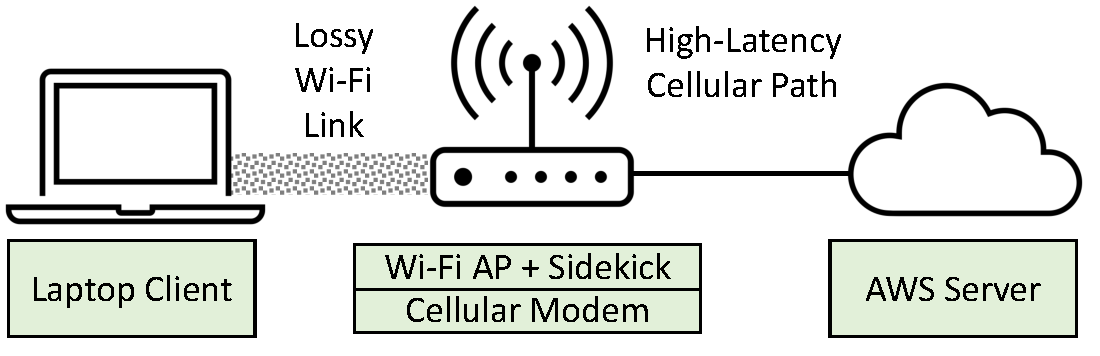
\includegraphics[width=0.7\linewidth]{sidekick/figures/setup_real.pdf}
\caption{Real-world experimental setup.
}
\label{fig:sidekick:real-setup}
\end{figure}


We modeled the scenarios from \Cref{sec:sidekick:motivating}. We use the same
m4.xlarge AWS instance as before for the emulated experiments.

\subsubsection{Emulation experiments.}

We emulated a two-hop network topology (\Cref{fig:sidekick:overview}) in mininet,
configuring the link properties using \texttt{tc}.
In emulation, we represented
each link by a constant delay (with variability induced by the queue), a random
loss percentage, and a maximum bandwidth.
\Cref{tab:sidekick:experimental-scenarios} describes the parameters
for each link to model---e.g., lossy Wi-Fi or a high-latency cellular
path---as well as the metrics for success in that scenario.
Link 1 connects the data sender (client) to the proxy,
while Link 2 connects the proxy to the data receiver (server).
On the proxy, we either run a Sidekick,
a connection-splitting TCP PEP~\cite{caini2006pepsal}, or nothing at all.

\subsubsection{Real-world experiments.}

To test its robustness, we also evaluated the Sidekick protocol over a real-world
environment that resembled the scenario on the train (\Cref{fig:sidekick:real-setup}).
In this setup, a Lenovo ThinkPad laptop, running Ubuntu 22.04.3 with a 4-Core
Intel i7 CPU @ 2.60 GHz and 16 GB memory, acted as a client to an AWS instance in
the nearest geographical region. The ThinkPad used as an access point (AP)
a Lenovo Yoga laptop, running Ubuntu 20.04.6 with a 4-Core Intel i5 CPU @
1.60 GHz and 4 GB memory, with a 2.4 GHz Wi-Fi hotspot.
The AP was connected to the Internet via a JEXtream cellular modem
with a 5G data plan. The AP ran Sidekick software.

We measured the link properties of each path segment to compare to
our emulation parameters. We measured delay and loss using 1000~\texttt{ping}s
over a 100 second period, and bandwidth using an \texttt{iperf3} test.
On the near segment between the ThinkPad client and the AP,
the min/avg/max/stdev RTT was 1.249/37.194/272.168/54.660 ms
at 49.8 Mbit/s bandwidth. We observed that loss increased
the further away the AP. In our experiments, the client was located roughly
200 feet away in a different room, with 3.6\% loss.
The far segment between the AP and the AWS server was
48.546/64.381/92.374/6.806 ms with 0.0\% loss at 30.9 Mbit/s.
In both environments, the cellular link was the bottleneck link in terms of
bandwidth, and the corresponding path segments in emulation had similar
minimum RTTs and average loss percentages.

\section{Real-world results}
\label{sec:sidekick:real-world}

\begin{figure}[t]
\centering
\begin{subfigure}{0.48\linewidth}
	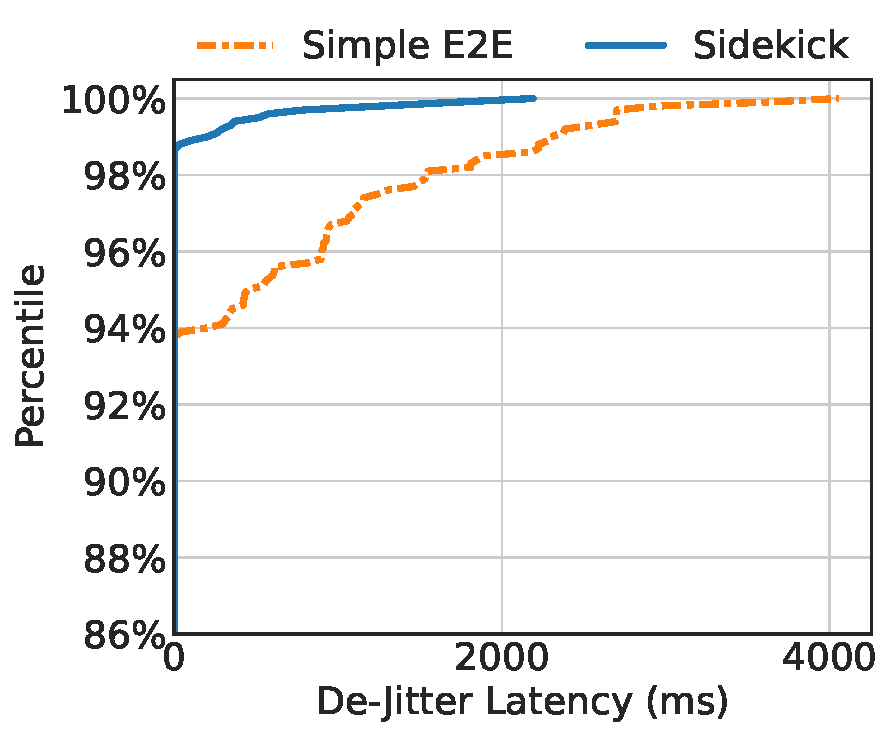
\includegraphics[width=\linewidth]{sidekick/figures/fig8_real_world_webrtc.pdf}
	\caption{Low-latency media. CDF of per-packet de-jitter
	latencies over 10 one-minute trials per protocol.}
	\label{fig:sidekick:real-world:media}
\end{subfigure}
\begin{subfigure}{0.48\linewidth}
	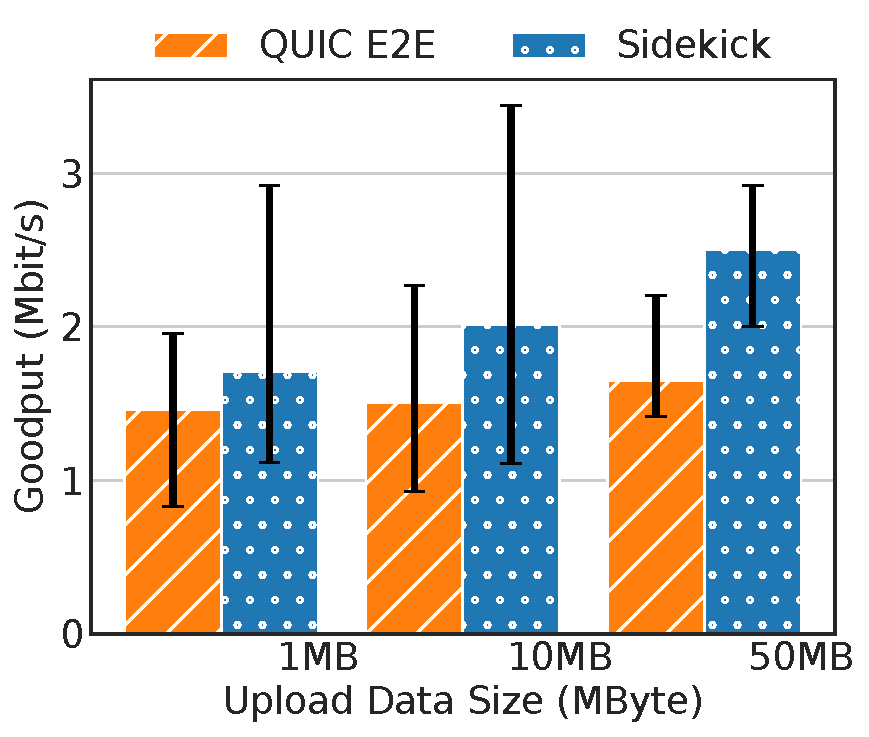
\includegraphics[width=\linewidth]{sidekick/figures/fig8_real_world_retx.pdf}
	\caption{Path-aware congestion control.
	Median of 20 trials. Error bars are 1st and 3rd quartiles.}
	\label{fig:sidekick:real-world:pep-emulation}
\end{subfigure}
\caption{Real-world results. Experiments were run in a moderately well-attended
office environment over a Friday afternoon. Trials alternate between the
baseline and the Sidekick to account for variability in time of day.
}
\label{fig:sidekick:real-world}
\end{figure}


We discuss the results of our experiments replicating two of our scenarios in
the real world, using as context
these main differences between emulation and the real-world:

\begin{itemize}[noitemsep,topsep=0pt]
  \item The RTT is more variable as it depends on interactions in the
  wireless medium and the shared cellular path.
  \item Wireless loss can be more variable as nearby 2.4 GHz devices and
  physical barriers may interfere with the link. Wireless loss also tends
  to be more clustered in practice.
  \item The available bandwidth on the shared cellular path is more variable,
  and depends on the time of day.
\end{itemize}

\Cref{fig:sidekick:real-world} shows the results of running the low-latency media and
connection-splitting PEP emulation experiments in the real-world. The baseline
protocol with a Sidekick is able to
reduce the 99th percentile de-jitter latency of an audio stream
from 2.3~seconds to 204~ms---about a 91\% reduction---and
improve the goodput of a 50 MB HTTP/3 upload by about 50\%.
Although the improvements are more conservative compared to emulation in
\Cref{fig:sidekick:main-results:media} and
\Cref{fig:sidekick:main-results:pep-emulation}, each case still benefits the
base protocol under all circumstances, compared to end-to-end mechanisms alone.

Part of the difference can be attributed to the network setting. When there is
no loss on the near path segment, as can occasionally happen in a real Wi-Fi link,
we do not expect to
see a difference with a Sidekick. When there is more loss on the far path segment, which
is variable and depends on the time, we
expect the benefit of the Sidekick to be less since this equally affects the
performance of the base protocol.

The other part of the difference could be made up by future work that better
adapts a Sidekick connection to real-world variability: The client could improve
path segment RTT estimation based on when the proxy receives packets, and use this
dynamic estimate in the calculation of $r$ used in $\beta$ and $C$.
The client could also use
this estimate to dynamically adjust the quACK interval.
Finally, we could analyze theoretically how PACUBIC responds
to traffic patterns in the real world.

\section{Emulation results}
\label{sec:sidekick:emulation}

\begin{figure*}
\begin{subfigure}{0.34\textwidth}
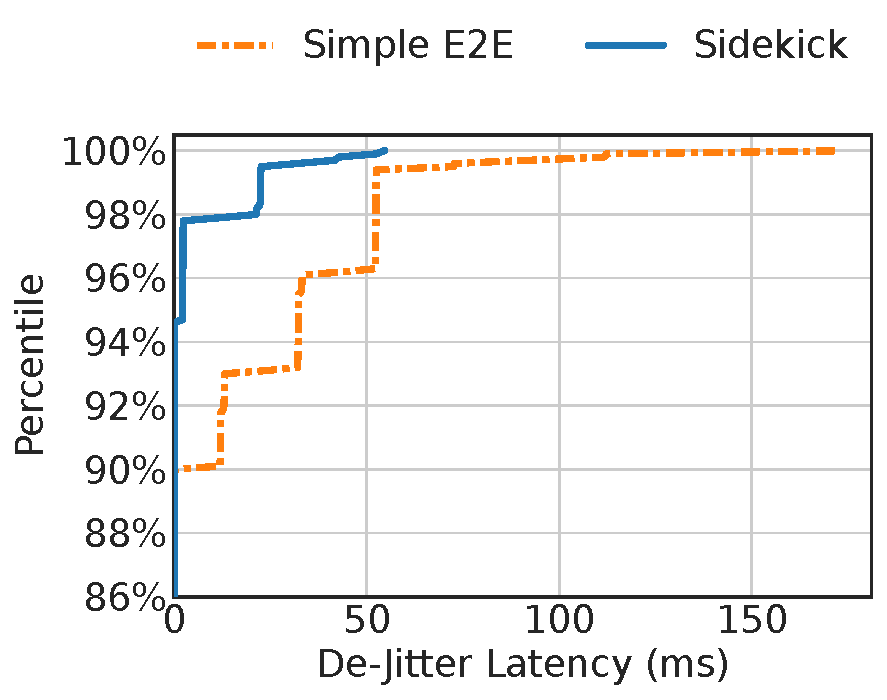
\includegraphics[width=\linewidth]{sidekick/figures/fig4a_low_latency_media.pdf}
\caption{Scenario \#1: Low-latency media.
 Reduced tail latency of de-jitter delay
with earlier retransmission. 5 minute trials.}
\label{fig:sidekick:main-results:media}
\end{subfigure}
\hfill
\begin{subfigure}{0.31\textwidth}
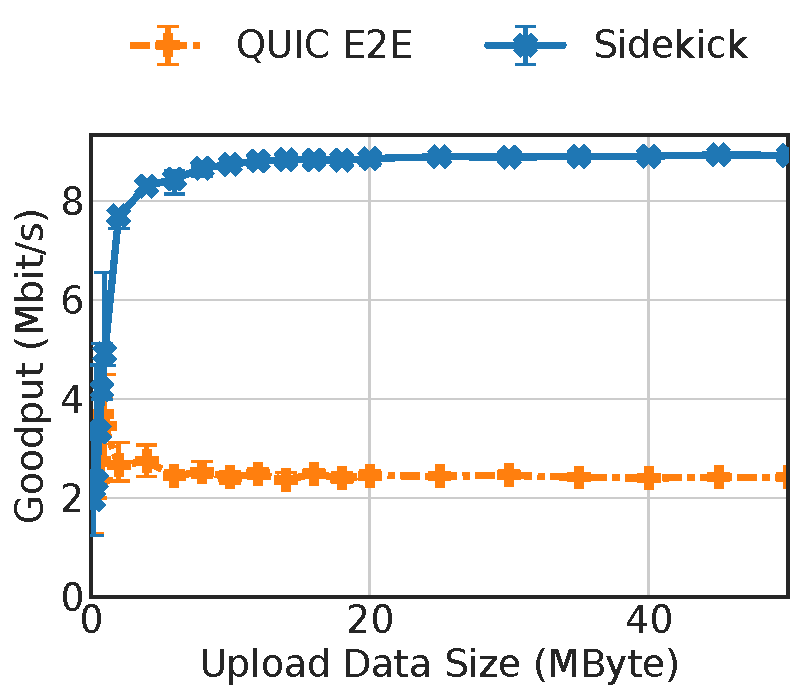
\includegraphics[width=0.97\linewidth]{sidekick/figures/fig4b_pep_emulation.pdf}
\caption{Scenario \#2: Connection-splitting PEP emulation. Improved goodput.
20 trials median. Error bars are 1st and 3rd quartiles.
}
\label{fig:sidekick:main-results:pep-emulation}
\end{subfigure}
\hfill
\begin{subfigure}{0.32\textwidth}
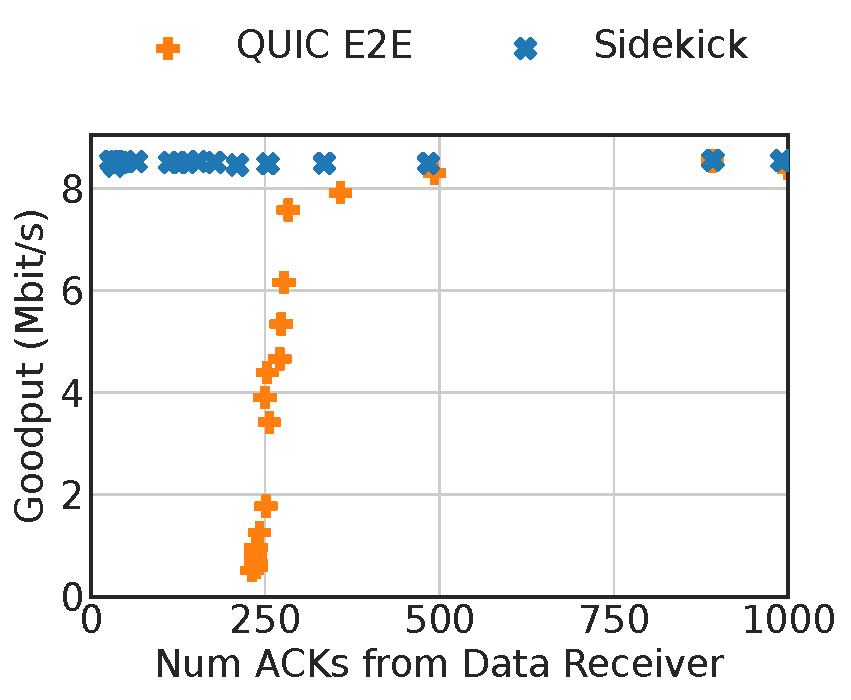
\includegraphics[width=0.99\linewidth]{sidekick/figures/fig4c_ack_reduction.pdf}
\caption{Scenario \#3: ACK reduction.
High goodput independent of end-to-end ACK frequency.
10 MB upload.}
\label{fig:sidekick:main-results:ack-reduction}
\end{subfigure}
\caption{
Comparing the end-to-end baseline protocol to the same protocol with a Sidekick
connection, using the success metrics for the three scenarios described in
\Cref{tab:sidekick:experimental-scenarios}. The \textsf{Sidekick($N$x)} data points show
the performance at $N$x the quACK interval (sent less frequently) and
threshold of the default configurations specified in
\Cref{tab:sidekick:experimental-scenarios}.
}
% \dm{Maybe a notation like $x/4$ would be more suggestive than $4x$?}
\label{fig:sidekick:main-results}
\end{figure*}


We evaluated our implementation of the Sidekick protocol in a more controlled
emulation environment to answer the following questions:
\begin{enumerate}[noitemsep,topsep=0pt]
	\item Can Sidekicks improve the performance of secure transport protocols
	in a variety of scenarios while preserving the end-to-end behavior of the
	base protocols?
	\item Can a path-aware congestion control algorithm match the fairness of
	split TCP PEPs using CUBIC?
	\item How do the CPU overheads of encoding quACKs impact the maximum
	capacity of a proxy with a Sidekick?
	\item What link overheads does the power sum quACK add and how does it
	compare to the strawmen?
\end{enumerate}

\subsection{Performance of secure transport protocols with Sidekick}
\label{sec:sidekick:emulation:performance}

We first evaluate Sidekick's main performance goal: In each of the motivating
scenarios, we show that the Sidekick protocol can improve performance compared
to the base protocol alone, which would not be able to benefit from existing
PEPs. Each scenario has a different metric for success---tail latency,
throughput, or number of packets sent by the data receiver (corresponding to
energy usage or chance of Wi-Fi collisions)---demonstrating the versatility of
the Sidekick protocol.

\subsubsection{Low-latency media application.}
The Sidekick can reduce tail latencies in a low-latency media stream, representing
fewer drops and better quality of experience.
The early retransmissions induced by the Sidekick reduced the 99th percentile
latency of the de-jitter buffer delay from 48.6 ms to 2.2 ms---a 95\%
reduction (\Cref{fig:sidekick:main-results:media}).
As long as the quACK interval is less than the end-to-end RTT, the connection
benefits from the Sidekick.

The Sidekick is beneficial in this scenario because it enables the client to sooner
detect and retransmit lost packets, and the server to sooner play packets from
its de-jitter buffer.
The end-to-end mechanism takes one additional received packet to notify of the
loss and
one end-to-end RTT to retransmit and play the packet (20+52=72ms), resulting in
three delayed packets (the three ``steps" in \Cref{fig:sidekick:main-results:media}) in most cases.
The Sidekick takes up to two additional packets and one near path segment RTT
(20+2=22ms or 20$\times$2+2=42ms), delaying either one or two packets in comparison.
Dropped ACKs and quACKs account for the $<2\%$ of packets with even greater
de-jitter latencies.

\subsubsection{Connection-splitting PEP emulation.}
The Sidekick improves upload speeds when there is a lossy, low-latency link
by using quACKs to inform the sender's congestion control.
In a scenario with $1\%$ random loss on the link between the proxy and the
data sender, the HTTP/3 (QUIC) client achieves $3.6\times$ the goodput for a 10 MB
upload with a Sidekick compared to end-to-end QUIC (\Cref{fig:sidekick:main-results:pep-emulation}).

When there is no random loss, the Sidekick does not impact the performance
of QUIC\@.
There are no logical changes to the base protocol in this case because all loss
is on the
bottleneck link on the far path segment, and the CPU overheads of processing quACKs
are negligible.

Knowing \emph{where} congestion occurs is an opportunity for creating smarter
congestion control. In PACUBIC, identifying where the loss occured let the data
sender reduce the congestion window proportionally to how many packets were
in-flight on each path segment. In \Cref{sec:sidekick:emulation:pacubic}, we
will show that our path-aware congestion control algorithm still matches the
fairness of connection-splitting TCP PEPs.

\subsubsection{ACK reduction scenario.}

Using quACKs in lieu of end-to-end ACKs allows the data receiver to
significantly reduce its ACK frequency while maintaining high goodput.
In our experiment, QUIC with a Sidekick sent $96\%$ fewer packets (mainly ACKs)
than end-to-end QUIC before the goodput dropped below 8.5 Mbit/s
(\Cref{fig:sidekick:main-results:ack-reduction}).
The quACK enables the data sender to promptly move the flow-control window forward,
as long as the last hop is reliable.

The goodput significantly degrades when reducing the end-to-end ACK frequency
without a Sidekick. When end-to-end QUIC reduces the ACK frequency to every
80 ms, the data receiver sends $247 / 138 = 1.8\times$ the packets at
$4.5 / 8.4 = 0.5\times$ the goodput, worse than QUIC with the Sidekick
in both dimensions (\Cref{fig:sidekick:main-results:ack-reduction}). With a Sidekick,
the data sender also does not need to change packet pacing to avoid bursts in
response to infrequent ACKs, which is why end-to-end QUIC cannot send fewer
than $\approx 240$ packets.

\subsubsection{Discussion: Configuring the Sidekick connection.}
\Cref{tab:sidekick:experimental-scenarios} shows the quACK interval and threshold we
elected for each scenario based on the considerations in
\Cref{sec:sidekick:init}. In each experiment in \Cref{fig:sidekick:main-results},
we also show how with less frequent quACKs ($2\times$ and $4\times$ the
interval) and proportionally-adjusted thresholds, the protocol performs worse,
or more variably. Less frequent quACKs means the client reacts later to
feedback about the near path segment, and more often has to rely on the
end-to-end mechanism. The performance particularly degrades when the quACK
interval exceeds the end-to-end RTT. However, even in this case, the base
protocol with any Sidekick at all performs better than the base protocol alone\@.

\subsection{Link overheads from sending quACKs}
\label{sec:sidekick:emulation:link-overheads}

\begin{table}[ht]
\begin{subtable}{\columnwidth}
  \setlength{\tabcolsep}{2pt}
  \centering
  \begin{tabular}{lccccccc}
    \toprule
    & \multicolumn{2}{c}{Data Sender$\rightarrow$} & \multicolumn{2}{c}{$\leftarrow$Proxy} & \multicolumn{2}{c}{$\leftarrow$Data Receiver} & \\
    & \bf Pkts & \bf Bytes & \bf Pkts & \bf Bytes & \bf Pkts & \bf Bytes & \bf Goodput \\
    \midrule
    QUIC E2E & $1.00\times$ & $1.00\times$ & $1.00\times$ & $1.00\times$ & $1.00\times$ & $1.00\times$ & $1.00\times$ \\
    Strawman 1a & $0.96\times$ & $1.01\times$ & \cellcolor{LighterRed}{$2.02\times$} & \cellcolor{LightestRed}{$1.56\times$} & $1.01\times$ & $1.03\times$ & \cellcolor{LighterGreen}{$3.33\times$} \\
    Strawman 1b & $0.94\times$ & $1.00\times$ & \cellcolor{LighterRed}{$2.00\times$} & \cellcolor{LightestRed}{$1.78\times$} & $1.00\times$ & $1.03\times$ & \cellcolor{LightGreen}{$3.53\times$} \\
    Strawman 1c & \cellcolor{LightestRed}{$1.83\times$} & $1.06\times$ & \cellcolor{LighterRed}{$2.01\times$} & \cellcolor{LightestRed}{$1.83\times$} & $1.00\times$ & $1.03\times$ & \cellcolor{LightGreen}{$3.46\times$} \\
    \bf \textcolor{black!50!blue}{Power Sum}   & \textcolor{black!50!blue}{\bf 0.94$\times$} & \textcolor{black!50!blue}{\bf 1.00$\times$} & \textcolor{black!50!blue}{\bf 1.03$\times$} & \textcolor{black!50!blue}{\bf 1.07$\times$} & \textcolor{black!50!blue}{\bf 1.00$\times$} & \textcolor{black!50!blue}{\bf 1.03$\times$} & \cellcolor{LightGreen}{\textcolor{black!50!blue}{\bf 3.55$\times$}} \\
    \bottomrule
  \end{tabular}
  \caption{Scenario \#2: Connection-splitting PEP emulation.\\}
  \label{tab:sidekick:packet-overheads:retx}
\end{subtable}
\begin{subtable}{\columnwidth}
  \setlength{\tabcolsep}{2pt}
  \centering
  \begin{tabular}{lccccccc}
    \toprule
    & \multicolumn{2}{c}{Data Sender$\rightarrow$} & \multicolumn{2}{c}{$\leftarrow$Proxy} & \multicolumn{2}{c}{$\leftarrow$Data Receiver} & \\
    & \bf Pkts & \bf Bytes & \bf Pkts & \bf Bytes & \bf Pkts & \bf Bytes & \bf Goodput \\
    \midrule
    QUIC E2E & $1.00\times$ & $1.00\times$ & $1.00\times$ & $1.00\times$ & $1.00\times$ & $1.00\times$ & $1.00\times$ \\
    Strawman 1a & $0.96\times$ & $1.00\times$ & \cellcolor{LightRed}{$9.94\times$} & \cellcolor{LighterRed}{$4.99\times$} & \cellcolor{LightGreen}{$0.04\times$} & \cellcolor{LightGreen}{$0.08\times$} & $1.02\times$ \\
    Strawman 1b & $0.96\times$ & $1.00\times$ & \cellcolor{LightRed}{$9.95\times$} & \cellcolor{LightRed}{$7.13\times$}      & \cellcolor{LightGreen}{$0.04\times$} & \cellcolor{LightGreen}{$0.08\times$} & $1.02\times$ \\
    Strawman 1c & \cellcolor{LightestRed}{$1.91\times$} & $1.05\times$ & \cellcolor{LightRed}{$9.73\times$} & \cellcolor{LightRed}{$7.41\times$}      & \cellcolor{LightGreen}{$0.04\times$} & \cellcolor{LightGreen}{$0.08\times$} & $0.97\times$ \\
    \bf \textcolor{black!50!blue}{Power Sum}    & \textcolor{black!50!blue}{\bf 0.96$\times$} & \textcolor{black!50!blue}{\bf 1.00$\times$} & \textcolor{black!50!blue}{\bf 1.09$\times$} & \cellcolor{LighterRed}{\textcolor{black!50!blue}{\bf 2.56$\times$}} & \cellcolor{LightGreen}{\textcolor{black!50!blue}{\bf 0.04$\times$}} & \cellcolor{LightGreen}{\textcolor{black!50!blue}{\bf 0.08$\times$}} & \textcolor{black!50!blue}{\bf 0.98$\times$} \\
    \bottomrule
  \end{tabular}
  \caption{Scenario \#3: ACK reduction.}
  \label{tab:sidekick:packet-overheads:ackr}
\end{subtable}
\caption{Link overheads for a 10 MB upload. The cells represent the multiplier
relative to the end-to-end QUIC baseline for each type of quACK\@.
Lower is better for number of packets and bytes sent on a link.
Higher goodput is better. The power sum quACK achieves the success metric
for each scenario without incurring the link overheads of the strawmen.
We did not evaluate the contrived protocol in Scenario \#1.
}
\label{tab:sidekick:packet-overheads}
\end{table}


The other cost in terms of using Sidekick protocols is the additional data
sent by the proxy to the data sender.
Too many additional bytes use up bandwidth, and additional packets use
up CPU\@.
\Cref{tab:sidekick:packet-overheads} shows the number of packets and bytes sent at each
node comparing the strawmen and power sum quACK to no Sidekick connection at all.

Using power sum quACKs increases the packets sent from the proxy to the data
sender
by 3-9\%. These packets either consist mostly
of end-to-end ACKs which are sent every packet in \texttt{quiche}, or end-to-end
ACKs that have been replaced by quACKs in the ACK reduction scenario.
We did not evaluate Scenario \#1 because it is based
on a contrived protocol that lacks many of these features, and the link
overheads would not really make sense.

This overhead is representative of the CPU overhead at the client, since
quACKs and ACKs take a similar number of cycles to process. In an experiment
with Scenario \#2 during a period of $\approx90$k incoming packets, ACKs took on
average 26065 cycles to process while the quACKs took 26369 cycles, 1\% more.
These cycles come from, i.e., the complex recovery and loss detection algorithms
implemented at the end host.

The strawmen have significantly higher link overheads compared to the power sum
quACK\@. The proxy sends up to 10$\times$ more packets using Strawman 1a, and
also slightly harms the goodput in the congestion control scenario.
The reduced goodput is due to the sender mis-identifying received packets as
dropped due to dropped quACKs.
The proxy achieves higher goodput with Strawman 1b but sends
more bytes. Strawman 1c increases the link overheads at both the proxy and the
data sender due to larger TCP headers and TCP ACKs.
We did not evaluate Strawman 2 due to its impractical decode time.

\subsection{CPU overheads of encoding at the proxy}
\label{sec:sidekick:emulation:cpu-overheads}

\begin{table}[ht]
  \centering
  \begin{tabular}{lrrrr}
    \toprule
    & \multicolumn{2}{r}{\bf 25-Byte Payload} & \multicolumn{2}{r}{\bf 1468-Byte Payload}\\
    & \bf Cycles & \bf $\%$ & \bf Cycles & \bf $\%$ \\
    \midrule
    Sniff Packet & 22417 & 97.6 & 22408 & 97.5 \\
    Table Lookup &   247 &  1.1 &   251 &  1.1 \\
    Parse ID     &    23 &  0.1 &    22 &  0.1 \\
    Encode ID    &    74 &  0.3 &    69 &  0.3 \\
    Other        &   213 &  0.9 &   225 &  1.0 \\
    \midrule
    \emph{Total} & \emph{22974} & \emph{100.0} & \emph{22975} & \emph{100.0} \\
    \bottomrule
  \end{tabular}
  \caption{Breakdown of the CPU cycles spent processing each packet at the
  proxy. Most cycles are spent on general per-packet overheads as opposed to
  quACK-specific processing.
  }
  \label{tab:sidekick:cpu-overheads}
\end{table}


The main bottleneck of Sidekick on a proxy is the CPU\@.
\Cref{tab:sidekick:cpu-overheads} shows a breakdown of the number of CPU cycles in each
step. The largest overhead was reading the packet contents from the network
interface ($97.5\%$ of the CPU cycles).

Encoding an identifier in a power sum quACK with $t=10$ used $74$ CPU
cycles ($0.9\%$). As a calculation of the theoretical maximum on a 2.30 GHz
% 2.30e9 / 74 = 31 million
CPU, the proxy would be able to process $31$ million packets/second on a single
core. The hash table lookup used $251$ cycles and parsing the pseudorandom
payload as an identifier used $22$ cycles.

In practice, we measured the maximum throughput of our Sidekick proxy to
be 464k packets/s with 25-byte payloads and 5.5 Gbit/s (458k packets/s) with
1468-byte packet payloads on a single core (assuming 1500-byte MTUs).
This experiment used multiple \texttt{iperf3} clients to simulate high
load until the proxy was unable to keep up with the load on a single core.
The packet payload size did not seem to affect results.

We find these achieved throughputs acceptable for edge routers such as Wi-Fi APs
and base stations. To deploy the Sidekick proxy on core routers, we would need
to reduce the overhead of reading packets from the NIC, such as by bypassing
the kernel/user-space protection boundary\footnote{ A kernel-bypass system like
Retina~\cite{wan2022retina} can achieve 25 Gbps on 2 cores while processing raw
packets with a 1000-cycle callback(Figure 5(a) in \cite{wan2022retina}). The
Sidekick equivalent would be a 500-cycle callback, and assuming all traffic has
requested Sidekick help. Throughput scales almost linearly with the number of
cores using symmetric RSS hashing. Thus we don't expect proxy overheads to be
an issue with modern 100 Gbps network speeds and an optimized implementation
even on commodity hardware. }~\cite{dpdk,mccanne1993bsd,wan2022retina} or using
native hardware~\cite{bosshart2014p4}. We could also scale on multiple cores
using symmetric RSS hashing~\cite{woo2012scalable}.

\subsection{TCP friendliness of path-aware CUBIC}
\label{sec:sidekick:emulation:pacubic}

\begin{figure}[t]
\centering

\includegraphics[width=\columnwidth]{sidekick/figures/fig5_baseline_bar_legend.pdf}
\begin{subfigure}{0.49\linewidth}
	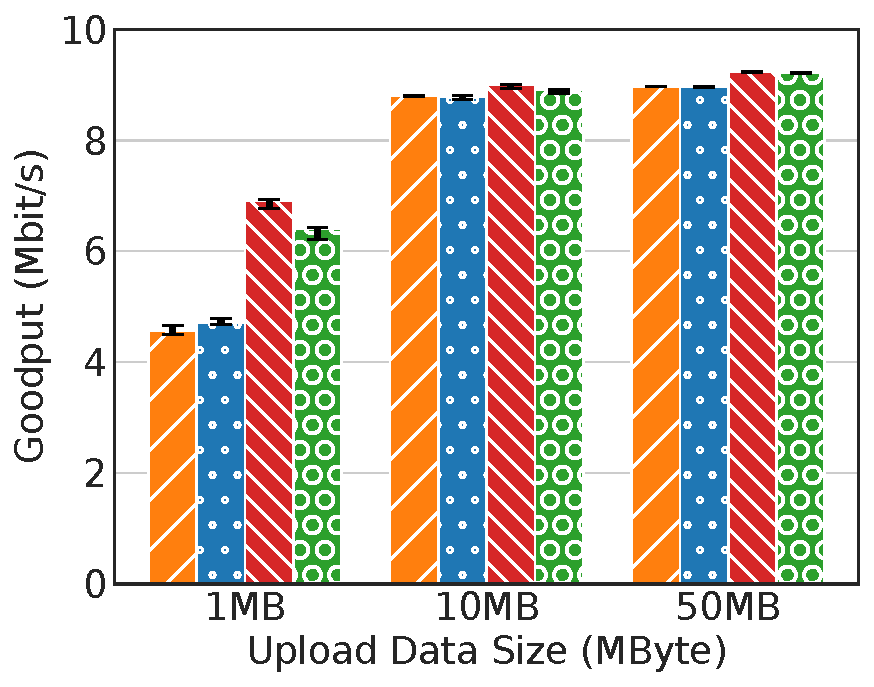
\includegraphics[width=\linewidth]{sidekick/figures/fig5_baseline_loss0p.pdf}
	\caption{0\% loss.}
	\label{fig:sidekick:fairness-bar:loss0p}
\end{subfigure}
\begin{subfigure}{0.49\linewidth}
	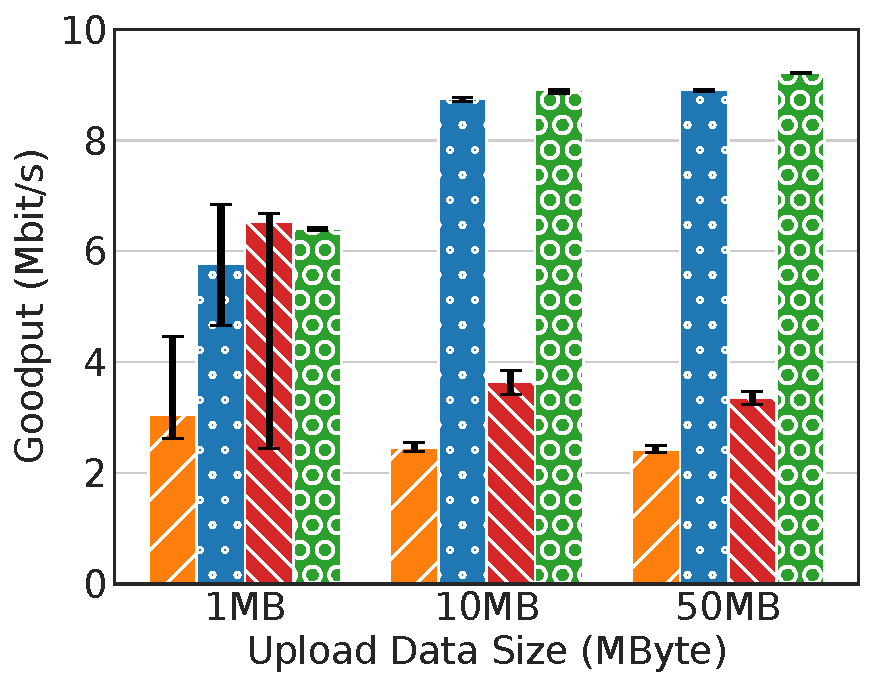
\includegraphics[width=\linewidth]{sidekick/figures/fig5_baseline_loss1p.pdf}
	\caption{1\% loss.}
	\label{fig:sidekick:fairness-bar:loss1p}
\end{subfigure}
\caption{Median goodput for three upload data sizes with $0\%$ and $1\%$ loss on
Link 1. 20 trials. Error bars are 1st and 3rd quartiles.
With proxy assistance at $1\%$
loss, both QUIC and TCP match the performance of when there is no loss at all.
}
\label{fig:sidekick:fairness-bar}
\end{figure}

\begin{figure}[t]
\centering

\includegraphics[width=0.8\columnwidth]{sidekick/figures/fig6_legend.pdf}
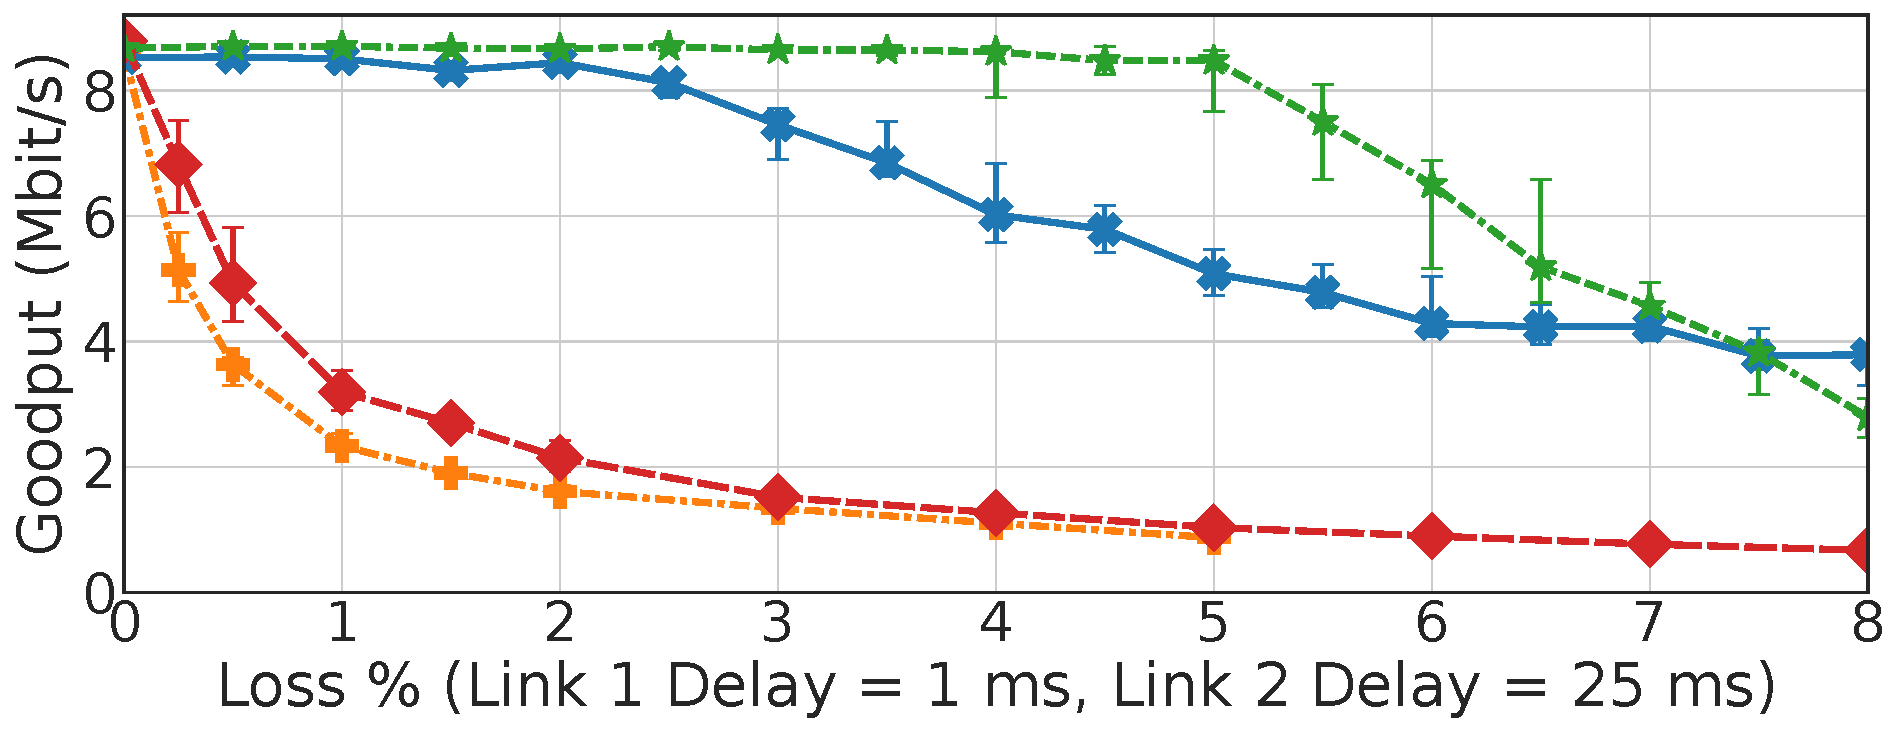
\includegraphics[width=0.8\columnwidth]{sidekick/figures/fig6_loss_bw100_10M_delay_25ms_1ms.pdf}
\caption{Connection-splitting PEP emulation as a function of near-segment
	loss rate. In this emulation experiment, QUIC+Sidekick (running PACUBIC)
  performs similarly to TCP+PEP (each connection running CUBIC)
  and improves goodput compared with end-to-end protocols. The graph shows
  median goodput of a 10~MByte upload. QuACK interval is 30~ms, threshold
is 10. Error bars show IQR of 10 trials.
}
\label{fig:sidekick:fairness-line}
\end{figure}


It is easy to improve performance without regard to competing flows;
however, we demonstrate that PACUBIC can
match the fairness of split CUBIC in a TCP PEP connection\@.
We evaluate fairness using Scenario \#2 with varying amounts of loss on the
near path segment.

\subsubsection{QUIC vs.\ TCP\@.}
We first compare QUIC to TCP without either PEP\@.
As both connections use CUBIC, they exhibit similar
congestion control behavior and achieve nearly maximum throughput in the
emulated network with no random loss (\Cref{fig:sidekick:fairness-bar:loss0p}).
We attribute the differences to the slightly different retranmission and
loss recovery behaviors of QUIC and TCP\@. The PEPs do not affect the
performance.

With even a little loss on the near path segment, both QUIC and TCP dramatically
worsen, respectively achieving $28\%$ and $42\%$ of the goodput at $0\%$ loss,
for a 10 MB upload (\Cref{fig:sidekick:fairness-bar:loss1p}).
% 0.305 / 1.098 = 27.8%
% 0.467 / 1.121 = 41.7%
In both protocols, CUBIC treats every transmission error as a congestion event,
even though no amount of reducing the congestion window affects the error rate.
QUIC and TCP perform similarly to each other with proxy assistance and 1\%
loss on the near path segment.

\subsubsection{Sidekick vs.\ TCP PEP\@.}
\Cref{fig:sidekick:fairness-line} shows that QUIC with a Sidekick roughly matches---as
 intended---the behavior of TCP with a PEP-assisted split connection. At higher
loss rates, the near path segment becomes the bottleneck link even with earlier
feedback about loss, causing the performance of TCP with proxy assistance to
drop. QUIC with a Sidekick follows a similar pattern because of its path-aware
congestion-control scheme (\Cref{sec:sidekick:sender}). The
results indicate that the Sidekick protocol's gains do not come at the expense
of congestion-control fairness relative to the split TCP connection.

\section{Summary}
\label{sec:sidekick:summary}


\chapter{Packrat Protocol}

The relationship between Internet transport protocols and lossy
wireless networks has long been fraught. Three decades ago, the
seminal Snoop work~\cite{balakrishnan1995snoop} addressed an issue
that emerged with the rise of wireless Ethernet (Wi-Fi): TCP's
end-to-end reliability works poorly over network segments that
regularly experience non-congestive packet loss. This is for two big
reasons: it's wasteful to require frequent end-to-end retransmissions
over a whole network path to address packet loss on one wireless link,
and because most congestion-control schemes interpret packet loss as a
sign of congestion and will slow down in response---a mistake when the
loss wasn't caused by congestion. From its point of view in 1995, the
Snoop paper outlined three plausible solutions:
\begin{itemize}[topsep=0pt,itemsep=0pt]
\item \textbf{Splitting TCP connections}~\cite{bakreitcp1994, bb95}. A
  proxy at the wireless base station transparently interposes on TCP
  connections that cross it, creating two concatenated connections:
  one from ``fixed host'' to proxy, and from proxy to the ``mobile
  host.'' This lets retransmission occur over the lossy segment only,
  and prevents the fixed host's congestion control from seeing
  non-congestive wireless losses.

\item \textbf{Link-level acknowledgment and
  retransmission}~\cite{palplus}. Wireless NICs add their own
  encapsulation (with their own sequence numbers or packet
  identifiers) to each packet, reply to incoming packets with
  link-layer acknowledgments, detect apparent losses from the absence
  of an ACK, and retransmit lost packets before the end-to-end
  transport protocol concludes they were lost.

\item \textbf{The Snoop approach}, where an on-path network function
  transparently interprets TCP acknowledgments in-flight, detects
  losses, retransmits packets over the lossy link only, and
  temporarily hides loss from the other host to avoid a duplicate
  retransmission.
\end{itemize}

In the intervening years, the first two approaches were widely
deployed. At the boundary between the wired Internet and a lossy
wide-area subpath (e.g.~a satellite or cellular network), network
operators used connection-splitting performance-enhancing proxies
(PEPs) to accelerate TCP connections crossing their networks. For
lossy \emph{local}-area subpaths, Wi-Fi and cellular networks use
link-layer sequence numbers, selective ``block'' acknowledgments,
link-layer retransmissions, and receiving NICs that sometimes hold
back received packets to wait for retransmissions of earlier packets
so that hosts receive packets in the original order to avoid
triggering a transport-layer end-to-end retransmission~\cite{rfc3366,
  rfc8985, 802.1ac, 5Greorder}. Because of the practical success of
the first two approaches, Snoop's ``network-originated
retransmissions'' didn't seem to be needed in practice.

Until, this paper proposes, maybe now. Post-TCP transport protocols,
especially QUIC~\cite{rfc9000}, encrypt and authenticate their
packets. This puts some operators in a bind, because they can no longer
``split'' these connections.
But what about link-layer ACKs and retransmissions?
This is a usable strategy on low-latency wireless links when one party
(or standards body) controls both sides, and losses can be patched
before the end-to-end protocol detects them. But when the lossy
subpath has higher latency (as for some satellite or experimental
networks), losses can't be patched before the transport protocol
detects them, and the head-of-line blocking necessary to put
packets back in order at the receiver can be ruinous to real-time
applications. In any event, such techniques can't be deployed
unilaterally by a network operator who doesn't control the receiver or
the encapsulation format.

What else could address this? Traffic sources could deploy
congestion-control and loss-detection schemes that are less sensitive
to loss and reordering~\cite{rfc8985}, but this is also out of a
network operator's control. Yet another approach could involve
Sidekick proxies~\cite{yuan2024sidekick}---but these provide
in-network \emph{acknowledgments} of encrypted transport protocols
(for hosts to interpret and perhaps trigger retransmission), not
in-network \emph{retransmission} based on the encrypted traffic of
hosts.

Given all this, what really happens today, at least some
of the time, is that satellite and other nontraditional network
operators block QUIC traffic, forcing hosts to fall back to TCP that
can be split as before. We think it may be possible to do better by drawing on ``Snoop-style''
ideas. In this paper, we describe and evaluate Packrat\footnote{For
``packet rateless retransmission''---and because the Packrat proxy keeps
a small cache of recent packets-in-flight for possible
retransmission.}: a technique for network-originated retransmissions
for encrypted end-to-end transport connections, yielding performance
benefits in lossy settings. We adapt set-reconciliation techniques
based on the Rateless IBLT~\cite{yang2024practical} to let the
receiver efficiently acknowledge encrypted packets (in an ``eACK'') to a network
function, without modifying the sender or the underlying wire
format. Compared with Sidekick, which also involves
acknowledgments over encrypted sequence numbers, these eACKs
are faster to decode, making them appropriate for a deployment
where network functions are the ones interpreting acknowledgments over
encrypted sequence numbers from many connections in parallel and
triggering retransmissions as a result.

% \begin{figure}
%     \centering
%     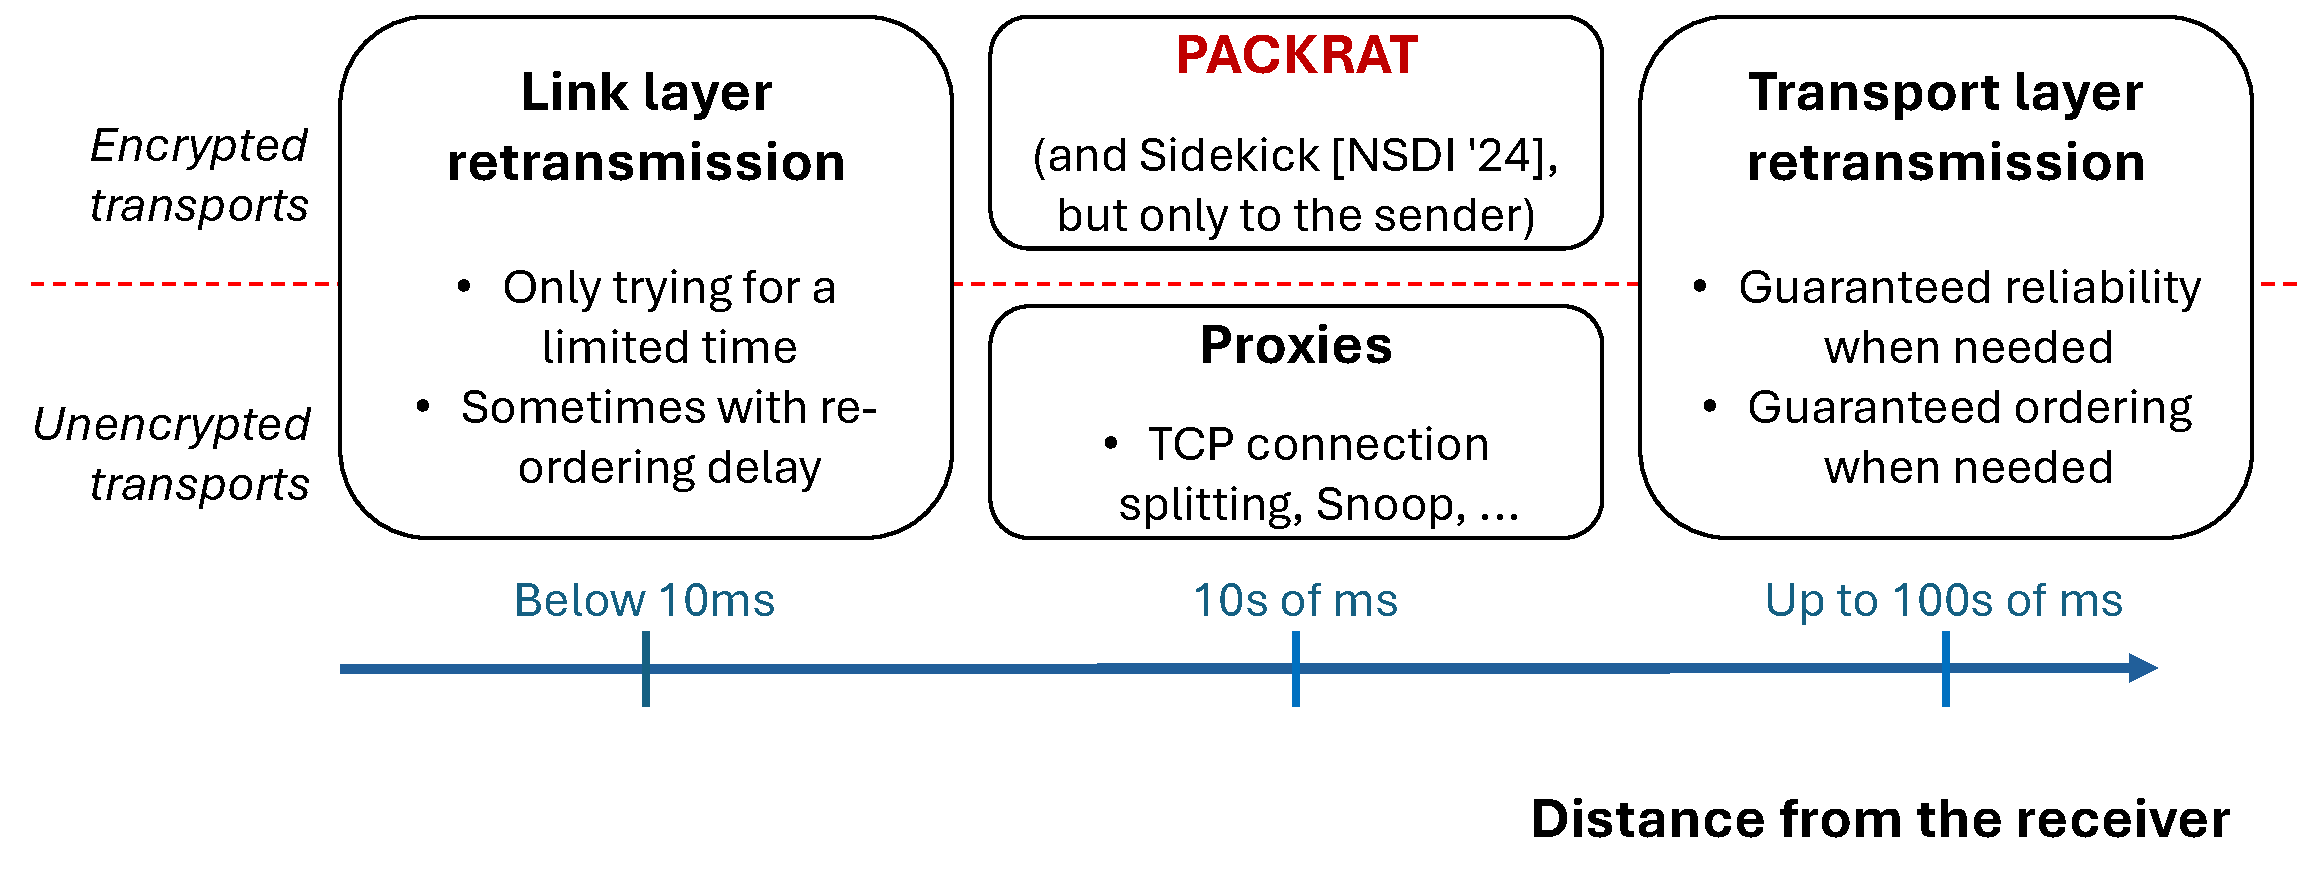
\includegraphics[width=\linewidth,height=35mm]{figures/packrat-scope.pdf}
%     \caption{Just a suggestion from Michael, to include a diagram like this. The editable pptx file is in the figures folder.}
%     \label{fig:packrat-scope}
% \end{figure}

We integrate the Packrat protocol with several applications built on encrypted
transport protocols, and show that it can enable a variety of performance
enhancements in various settings with a lossy path segment near the data receiver,
compared to end-to-end loss recovery schemes:

\begin{enumerate}[noitemsep]
\item Application 1: Improved throughput for large file downloads using QUIC and HTTP/3.
\item Application 2: Reduced packet tail latency of a low-latency media stream using a simple repetition code.
\item Application 3: Reduced end-to-end retransmissions at the server of a reliable multicast RTP stream.
\end{enumerate}

\noindent Unlike link-layer retransmissions, the assistance from a Packrat can be
deployed anywhere along the network path and tailored to the performance
demands of each base connection. Compared to existing transport-layer
solutions, Packrat can be applied to arbitrary transport protocols without
ossification.

\paragraph{Summary of results.}
To summarize, we show that it is possible to provide per-connection in-network
retransmissions to encrypted transport protocols using the Packrat protocol along
an adjacent connection, without involving the data sender nor modifying the
wire format of the underlying connection. We make the following contributions:

\begin{itemize}[noitemsep]
    \item The Packrat protocol and a mechanism at the \textit{endpoint} to correct
     end-to-end reordering signals when there are in-network retransmissions
     (\Cref{sec:packrat-protocol}).
    \item An acknowledgment of encrypted packets based on the Rateless IBLT
     that is fast to decode (\Cref{sec:eack}).
    \item Optimizations to improve proxy
     scalability based on the co-location of the endpoint and eACK sender
     (\Cref{sec:eack:hints}).
    \item An implementation of the Packrat proxy and integrations with three
     applications that use encrypted transport (\Cref{sec:implementation}).
    \item An emulation study of the performance enhancements, as well as the CPU,
     memory, and link overheads of using the Packrat protocol (\Cref{sec:evaluation}).
\end{itemize}

\section{Background: In-Network Retransmissions}

We provide a brief history of loss recovery mechanisms in the network to
motivate the need for lightweight, non-ossifying, in-network retransmissions
for encrypted transport protocols.

\paragraph{End-to-end loss recovery.}

In end-to-end loss recovery,
congestion control algorithms were traditionally designed to treat all loss as an indicator of
congestion~\cite{rfc5681tcp,rfc2001tcp}.

With modern wireless networks and higher bit-error rates, recent developments
such as the BBR congestion control
% (Bottleneck Bandwidth and Round-trip propagation time)
algorithm have de-prioritized packet loss as a congestion
signal~\cite{cardwell2017bbr}. This change enables higher throughput but has
raised concerns regarding TCP fairness~\cite
{ware2019modeling,philip2024prudentia}. In response, the performance of newer
versions of BBR has regressed in lossy environments, suggesting a lasting trend
in the treatment of loss as a congestion signal regardless of its source~\cite
{atc-submission}.

\paragraph{Link-layer loss recovery.}

Loss recovery at the link layer~\cite{3gpp5gstandard,le2022link,ieee80211e} can
mitigate some of the dramatic reactions of CCAs by hiding random loss from
endpoints.
Applications and transport protocols are oblivious to this
functionality, and there is a tradeoff to this reliability~\cite{klingler2018impact,kliazovich2012arqproxy}.
Retransmitting more often increases the chance
of success but increases the time needed, and may also introduce
jitter and reordering~\cite{leung2007overview}.
Low-latency applications may prefer to transmit new data instead, but
retransmitting less often means more loss.
There is no ideal configuration for all connections that share the link.

\paragraph{Transport-specific mechanisms.}

Some transport-layer proxies split a connection into two or more segments
and optimize the connection for each segment. In addition to
TCP connection splitters~\cite{rfc3135,honda2011still,hayes2019mmwave},
selective forwarding units (SFUs) are
used for media streams where low-latency is critical, so retransmissions occur
closer to the data receiver~\cite{rfc7667,andre2018comparative}.

With Snoop~\cite{balakrishnan1995snoop}, it is clear
that complexities emerge in how the proxy interprets
and modifies plaintext sequence numbers on the wire, which also ossifies TCP.
This paper aims to explore how such a proxy can send helpful in-network
retransmissions to a variety of encrypted protocols while preserving
end-to-end semantics, without access to such information.

These types of approaches make unwarranted assumptions about
transport headers ossify the protocol~\cite{papastergiou2017deossifying}.
By making reliability guarantees to the endpoint, the connection-splitting
proxies also fate share with the connection.

\paragraph{Protocol-agnostic transport assistance.}

Forward error correction can be used in lossy environments, but this
introduces significant overheads as entire packet contents (and not just
sequence numbers) must be encoded during transmission~\cite
{rfc9265}. FEC also requires participation from both endpoints.

Mechanisms that encapsulate packets offer potential for reliability without
decrypting packet contents, but their primary focus tends to be security. VPNs
introduce a costly encryption layer. MASQUE tunnels protocols over HTTP/3, and
if used for local retransmissions has the potential for complex nested loss
recovery and congestion control interactions~\cite
{rfc9298masque,schinazi-masque-proxy-05,kramer2021masquepep}. It is intended to
function per-application, and the best known implementation from Apple
functions like a VPN~\cite{icloud-private-relay}. These proxies may also not be
on-path, which harms performance.

The Sidekick proxy provides protocol-agnostic assistance by sending
``quACKs'' of encrypted packets to an endpoint, but cannot retransmit
packets itself~\cite{yuan2024sidekick}. This limits its usefulness
to when the loss is near the data \textit{sender}.
However, client traffic (which is near the lossy last-mile) is typically heavier
in the downlink direction. In this paper, we similarly leverage set
reconciliation in eACKs for referring to encrypted packets,
but to send network-originated retransmissions.

\section{The Reordering Problem}

\begin{figure}
    \centering
    \begin{subfigure}[b]{0.8\linewidth}
        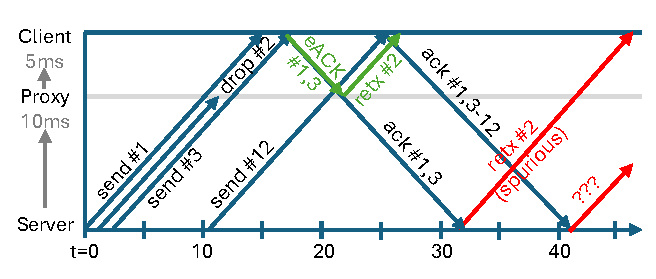
\includegraphics[width=\linewidth, trim=0 10 0 10, clip]{packrat-paper/figures/reordering_unmodified.pdf}
        \caption{Unmodified ACK.}
        \label{fig:reordering-problem:unmodified}
    \end{subfigure}
    \begin{subfigure}[b]{0.8\linewidth}
        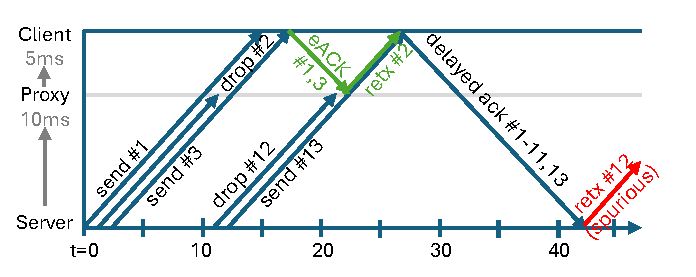
\includegraphics[width=\linewidth, trim=0 9 0 10, clip]{packrat-paper/figures/reordering_delayed_ack.pdf}
        \caption{Na\"ive delayed ACK.}
        \label{fig:reordering-problem:delayed-ack}
    \end{subfigure}
    \begin{subfigure}[b]{0.8\linewidth}
        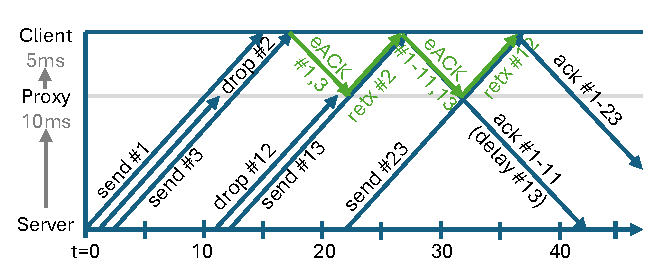
\includegraphics[width=\linewidth, trim=0 9 0 10, clip]{packrat-paper/figures/reordering_with_signal.pdf}
        \caption{ACK with Packrat reorder delay of 10 ms.}
        \label{fig:reordering-problem:packrat}
    \end{subfigure}
    \caption{\small The reordering problem where in-network retransmissions with
    millisecond RTTs cause the server to send spurious retransmissions. The
    end-to-end ACKs constructed with a Packrat reorder delay prevent this problem.
    \vspace{-0.4cm}
    }
    \label{fig:reordering-problem}
\end{figure}

Most acknowledgment schemes allow for some reordering but not at the level
incurred by in-network retransmissions. For example, TCP fast retransmit requires
three duplicate ACKs~\cite{rfc5681tcp}. The QUIC RFC specifies a threshold of three
out-of-order packets before detecting loss~\cite{rfc9002quic}. The RACK-TLP algorithm
allows for a time-based ``reordering window'', but still penalizes excessive
reordering~\cite{rfc8985}. Compared to, e.g., Wi-Fi retransmits, the
reordering from in-network transmissions is directly related to the RTT to
the proxy on the order of tens of milliseconds.
We call this the \textit{reordering problem}.

Consider an example using selective ACKs, where a gap is considered a missing
packet (\Cref{fig:reordering-problem:unmodified}): The server sends 1250-byte packets at 10 Mbit/s,
which is 1 packet every ms. The client drops packet \#2 but
receives \#1, \#3, \#4, etc. If the RTT between the client and proxy is 10 ms,
by the time the client receives the in-network retransmission of \#2 (from
eACKing \#1 and \#3), it could
have already ACKed $10$ more packets with higher sequence
numbers up to \#12. The server unnecessarily retransmits \#2 and treats the
loss as a congestion signal.
Spurious retransmissions take up valuable bandwidth and confuse congestion
control algorithms~\cite{leung2007overview}.

\paragraph{Na\"ive solutions.}

The Snoop protocol faces the same challenges with needing to modify end-to-end
signals when sending in-network retransmissions~\cite
{balakrishnan1995snoop}. The solution here involves withholding duplicate TCP
ACKs from the server if the proxy has the packet in the cache. However, without
plaintext sequence numbers, the Packrat proxy is unable to understand which
encrypted packets an encrypted end-to-end ACK is referring to, and can only
forward packets as intended.

Another option may be for the client to \textit{delay} sending an ACK until it
has allowed one proxy RTT for the proxy to retransmit the packet first~\cite{rfc3168}.
In the
previous example, the client may wait 10 ms from detecting the gap in
packet \#2 before sending an ACK, at which point it would have received the
retransmission for \#2 and be able to ACK the full range from \#1-13. This
seems promising at first, but in the time the client was waiting,
another loss could have occurred (\#12)
and the new ACK would have the same problem (\Cref{fig:reordering-problem:delayed-ack}).

Various other solutions exist, such as changing a server configuration, but it
is also undesirable to require certain features in all data senders as they
should not have to participate in the Packrat protocol.
% Various other na\"ive solutions exist, such as informing the server to increase
% its reordering threshold, but this requires it to be a configurable parameter
% in the base protocol. It is also undesirable to require certain features in all
%  data senders, as they should not have to participate in the Packrat protocol.

\paragraph{Packrat solution.}

Our solution is for the end-to-end ACKs constructed by the client to
signal \textit{jitter}, defined as variation in packet interarrival times,
instead of reordering. This enables the data receiver to process packets as
soon as they are received and reduces spurious retransmissions from the data
sender, without involving the data sender. The precise manifestation depends on
the acknowledgment scheme.

For example, QUIC ACKs consist of a cumulative sequence number, followed by SACK
ranges. Using Packrat, the QUIC ACK instead includes the cumulative sequence
number, but then only the ranges for packets that have been received for at
least the time it takes for the proxy to retransmit. This
\textit{reorder delay} includes the RTT to the proxy
as well as any delay in sending the eACK.
In the example, 10 ms after detecting the gap in \#2, the ACK consists
of packets \#1-2 and any cumulative sequence numbers beyond \#2 (up to \#11)
(\Cref{fig:reordering-problem:packrat}).
We assume
that most loss is near the client, and that the RTT to the proxy is less than
the loss detection timeout.

Different protocols use different acknowledgment schemes with similar flavors.
The modification for negative acknowledgments of missing packets is to delay
sending the NACK for at least one proxy RTT before deciding whether the NACK is
still needed. TCP relies on duplicate ACKs, which need a different
modification. Abstractly, packets are held and ordered in a jitter buffer for a
certain delay before they can be referenced in the client's underlying
acknowledgments.

\section{Packrat Protocol}

The Packrat protocol is spoken between a client and an on-path proxy, where the
client is a data \textit{receiver}. We imagine the proxy to exist near the data
receiver on the other side of a lossy path segment. This could be as close as
directly behind a Wi-Fi access point, at a cellular base station, or on the
first extraterrestrial node of a satellite network path. This is on the order
of 1s to 10s of milliseconds.

As an overview, once the client and proxy have established an adjacent
connection for a specific base connection identified by a UDP 4-tuple, the
proxy is ready to send in-network retransmissions. The client sends
acknowledgements of which encrypted packets it has received, and the proxy retransmits missing
packets it previously forwarded on that base connection.
But in-network retransmissions are not just that simple.

In the rest of this section, we start by describing the \textit
{reordering problem} with in-network retransmissions, and a mechanism at
the \textit{client} to address the issue. Then we describe the messages
exchanged between the client and proxy in the Packrat protocol to establish the
adjacent connection and generate in-network retransmissions,
and the behavior of each party in both the Packrat and base
connections. We assume each message is transmitted in an unreliable UDP
datagram.

\subsection{Proxy Behavior}

The behavior of the proxy is to decode incoming eACKs and retransmit missing
packets, and to cache and evict packets from the base connection for
retransmission. The state at the proxy for each base connection is (1) a packet
cache and (2) an eACK that represents the cumulative encoding of all packets
received by the client that are no longer in the cache.

\paragraph{Decode eACKs and retransmit.}

The \texttt{eACK} definitively states which packets have been \textit{received}
by the client. Based on its knowledge of which packets it has \textit{sent} to
the client, the proxy evicts any newly received packets from the cache. The
proxy then applies a loss detection policy to determine which of its sent
packets may have been dropped. The default
policy is any ``gap" in the ordered sequence of packets that were previously
cached, but packet timeouts could also apply. The proxy immediately retransmits
these missing packets, moving them to the top of the cache.

The retransmission is simply a duplicate of the original packet on the wire.
However, the proxy can also explicitly indicate that the retransmission comes
from the Packrat by encapsulating the UDP payload in a \texttt{Retransmit}. The
packet would be received by the client on the Packrat socket, which can then forward
the payload to the base connection.

\paragraph{Cache and evict packets.}

The proxy caches packets with the base connection 4-tuple in the order they are
forwarded to the client, up to the pre-configured cache size. It evicts packets
if an \texttt{eACK} indicates they have been received and no longer need to be
retransmitted. Whenever a packet is evicted, it is also encoded in the eACK
state of the base connection.

If a packet of the base connection arrives but the cache is full, the
proxy \textit{optimistically} evicts the oldest packets to make room. When
retransmissions are uncommon, this allows the client to eACK less frequently
and the proxy to maintain a significantly smaller cache. Unlike
connection-splitters, the proxy does not actually make reliability \textit
{guarantees}, and the client can always fall back to end-to-end retransmissions
after resetting the packrat connection, as described below.

\paragraph{Reset the packrat connection.}

If the proxy is unable to decode a eACK for any reason, it sends a \texttt
{Reset} to the client. These reasons include but are not limited to: an
insufficient number of symbols to decode the missing packets, a necessary
retransmission was optimistically evicted,
a packet corruption caused the encoded identifiers
to become out of sync, etc. The \texttt{Reset} indicates the start of a new
epoch in which the client and proxy encode identifiers into their eACKs.

Base connections that use the Packrat protocol must always be able to fall back to
end-to-end mechanisms when the Packrat is unable to send in-network
retransmissions. This is unlike typical connection-splitters and VPNs that fate
share with their endpoints. Similar to Snoop~\cite{balakrishnan1995snoop},
the Packrat style of in-network
assistance is better suited to mobility and handoffs if the connection ever
changes network paths.

\subsection{Data Receiver Behavior}

In addition to modifying end-to-end acknowledgments to avoid sending excessive
reordering signals to the server, the primary behavior of the client is
to \texttt{eACK} at a specified frequency, e.g., every 10 ms or every 16
packets. This frequency is typically the same as that of the underlying
acknowledgment scheme. The eACKs are cumulative representations of all the
packets ever received since sending the last \texttt{Init}.

\paragraph{Selective eACKing.}

An on-path proxy handles many tens to hundreds of thousands of concurrent
connections at once. Any per-packet overhead incurred by the Packrat protocol
at the proxy must be extremely small. The Packrat proxy encodes every packet in
the base connection and, unlike the Sidekick proxy, also decodes every
acknowledgment ($91\!\times$ more expensive than encoding in \cite
{yuan2024sidekick}). We want to explore whether a different type of
acknowledgment of encrypted packets can be more suitable in the setting of
in-network retransmissions for its computational efficiency.

If the client does not expect it needs a retransmission, there is not much point
in sending an eACK. In NACK schemes, where the client detects loss and asks for
a retransmission, it can choose to selectively eACK only when it would
otherwise send a NACK. Note that the client can omit regular eACKs without the
cache exploding in size because the proxy optimistically evicts packets, and
these are likely to be received or the client would have NACKed.\\

\section{Implementation}

We now describe our implementation of the Packrat protocol, which includes
the \texttt{eack} library (\Cref{sec:eack:microbenchmarks}),
a \texttt{packrat} library used for three client integrations,
and a Packrat proxy. We also describe the implementations of the
applications and baselines we use to evaluate Packrat.

\subsection{Applications}

We evaluate the Packrat protocol in three applications with different performance
metrics to explore the versatility of in-network retransmissions:
a high-throughput HTTP/3 file download, a low-latency media stream with forward
error correction, and a reliable multicast stream whose server has limited
capacity to handle end-to-end unicast retransmissions.

\paragraph{HTTP/3 file download.}

The HTTP/3 benchmark uses the default client and server in the Picoquic QUIC
implementation~\cite{picoquic}. Picoquic is an implementation of QUIC in C
based on the IETF standard used for experimentation on extensions to QUIC in
the IETF, with simplicity and correctness as its goals. Both endpoints use
CUBIC for congestion control.

The goodput is measured by dividing the connection time by the requested data
size, excluding headers.
The connection time is measured as when the client sends the first
byte of its request to when it receives all requested bytes.
We use 25 MB which is large enough such that the goodput is stable.

\paragraph{Low-latency media with FEC.}

We implement an endpoint for streaming low-latency audio data from the server
to the client, using a simple repetition code for forward error correction.
The server (a) sends a packet every 20 ms
(b) containing audio from the last 40 ms (so there's an overlap in each
packet). Each audio packet contains 480 bytes of data, representing an audio
stream at 96 kbit/s.

The client begins playback with 40 ms in its buffer, stalling if frames arrive
too late and fast-forwarding if behind the target buffer size.
If there is a gap in the
playback buffer, the client sends a NACK with the sequence number of the
missing frame. The client retransmits NACKs, up to one per RTT, until it has
received the missing frame. On receiving a NACK, the server immediately
retransmits.

The one-way latency is measured from the time the data is produced in the real
world to when it is encoded, transmitted, and available in the client's
buffer. For example, a frame containing 40 ms of data sent over a network path
with 150 ms delay has a minimum one-way latency of 190 ms.

\paragraph{Reliable IP multicast stream.}

The IP multicast application is similar to the low-latency media application
except the server streams data to a multicast IP address. The server does not
use forward error correction, and each packet contains 240 bytes of data. Multiple clients
subscribe to the multicast IP address, and if a client is missing data,
it sends an end-to-end NACK to the
multicast server to receive a unicast retransmission.
The primary metric is the number of end-to-end retransmissions requested by
the clients. That is, we measure the number of packets that the server
must (unicast) retransmit, which captures both server and network load.

\subsection{Client Integrations}

\begin{lstfloat}[t]
\begin{lstlisting}[language=Rust]
struct Packrat {
    /// Serialize a Packrat message to send
    fn send_init(params: ...) -> SendBuf;
    fn send_eack(); -> SendBuf;
    fn send_eack_rateless(m: usize); -> SendBuf;
    /// Handle the incoming message and return the
    /// payload if it is a `Retransmit` message.
    fn recv_payload(buf: RecvBuf) -> &[u8]
    /// Manage eACK state
    fn is_ready() -> bool;
    fn insert(id: u32) -> bool;
    fn reset();
}
\end{lstlisting}
\captionof{lstlisting}{Pseudocode interface for the \texttt{packrat} library.
 The library consolidates shared functionality at the client for sending
 eACKs. The client is responsible for reading and writing to the actual Packrat
 socket.}
\label{lst:quacker-interface}
\end{lstfloat}

Clients participate in the Packrat protocol by knowingly opting in to proxy
assistance and sending eACKs. Clients share much of the same functionality,
such as initializing the Packrat connection, maintaining a cumulative eACK of
received packets, and determining when to eACK based on a set frequency. We
implement a library for this shared functionality (\Cref{lst:quacker-interface})
and integrate it into our three clients.
The library uses $\approx\!700$ lines of Rust and includes C bindings.
% quacker$ cloc .

The library can serialize and deserialize messages in the Packrat connection, but
the client is responsible for reading and writing to the actual socket. Each
application uses a packet loop to interact with a socket for the base
connection. We incorporate the Packrat socket into the same loop, which allows us to
consider hints from the application for rateless and selective eACKing
(\Cref{sec:eack:hints}). We also incorporate a reorder delay in the base
connection (\Cref{sec:packet-protocol:problem}).

\subsection{Proxy Implementation}

We implement the Packrat proxy as a network bridge that uses raw sockets to read
and write packets between two interfaces. The proxy needs to
be on-path and intercept the packets, as opposed to sniffing them, so
its \texttt{InitACK} and \texttt{Reset} messages can be ordered along with the
data packets.

The proxy inspects each packet for magic discovery packets, those that match the
4-tuples of the base connections it is helping, and also eACKs.
It handles each packet as described in \Cref
{sec:packrat-protocol:proxy-behavior}. We use our \texttt{eack} library to
encode and decode eACKs. The proxy use $\approx\!1000$ lines of Rust.

\paragraph{Multicast proxy.}

We also implement an extension to the Packrat proxy for IP multicast, or more
generally, multiple clients that share a base data stream. The proxy maintains
a fixed-size cache for the multicast 4-tuple with optimistic eviction only. For
each client, the proxy maintains a eACK and a \textit{virtual cache}. The
virtual cache contains (1) a global index in the base cache of the client's
first unacknowledged packet and (2) pairs of global indexes that indicate which
packet to insert and where to insert it because it was retransmitted to the
client. This allows the proxy to maintain state proportional only to the number
of outstanding retransmissions per client.

\section{Evaluation}

We evaluate our Packrat protocol implementation in an emulation study and answer
the following questions:
\vspace{-0.2cm}
\begin{enumerate}[noitemsep]
    \item What are the performance advantages of the Packrat protocol over the
     end-to-end, connection-splitting, and tunnel baselines in network settings
     with a lossy path segment near the data \textit{receiver}?
    \item How do the rateless and selective optimizations in \Cref
     {sec:eack:hints} impact the link overheads of the Packrat protocol?
    \item How much memory does the cache use at the proxy?
    \item How much traffic can a CPU-constrained proxy handle?
\end{enumerate}

\subsection{Methodology}

The primary baseline is just the end-to-end protocol, which is the default for
encrypted transport protocols that cannot receive transport-layer assistance
from proxies.

We additionally aim to compare Packrat to link-layer loss recovery approaches,
as discussed in \Cref{sec:background}.
To mimic these approaches,
we implement a reliable tunnel that
encapsulates and retransmits packets
similar to Wi-Fi. The tunnel sender encapsulates IP datagrams in a header with
a plaintext sequence number, and the tunnel receiver replies with a 64-bit
Block ACK~\cite{ieee80211e}. The sender retransmits gaps in the acknowledgment up
to $7$ times, the default limit in Wi-Fi, and takes care to avoid duplicates. We
also implement an option for the receiver to order packets before releasing
them to the application, behavior that we believe is unspecified in the Wi-Fi
standard but can dramatically impact application performance.
We refer to these variants as ordered and unordered tunnels.

Finally, we benchmark our HTTP/3 application against a ``true'' split
connection. We implement a \texttt{picoquic} connection splitter that decrypts
and re-encrypts packets in two separate QUIC connections from one endpoint to
another. We emphasize that these connection-splitters do not actually exist. To
be deployed, the proxy would need to be credentialed with access to underlying
sequence numbers, the antithesis of the transport purists who encrypted these
headers in the first place~\cite{duke2023rfc}. Since TCP splitters \textit
{are} commonly deployed~\cite{honda2011still,rfc3135}, our goal is to
understand how much QUIC is ``losing out'' by not splitting its connection, and
how closely Packrat can help QUIC achieve the same performance benefits without
ossification.


\paragraph{Network configuration.}

We run emulation experiments in \texttt{mininet} to evaluate the Packrat protocol
in a controlled environment. We generally use a linear, two-segment network
topology.
The host nodes
correspond to the client, proxy, and server. Each segment has a bridging
node to emulate network properties on the link. In the multicast application,
we replicate the client and link it to the same bridging node.

We parameterize each path segment in three dimensions: delay, bandwidth, and a
random loss rate. We configure the network properties on the bridging nodes’
egress interfaces, using \texttt{tc-netem} to set delay and random loss,
and \texttt{tc-htb} to set bandwidth. Additionally, we use \texttt{tc-qdisc} to
configure the queues to use \texttt{red}, emulating congestive loss in our
single-flow environment. The links are symmetric.

In the end-to-end setting, the proxy simply runs a Linux transparent bridge.
Otherwise, the
proxy runs a binary for Packrat, the connection splitter, or the tunnel, that
manually bridges traffic between the two interfaces.
In the tunnel proxy case, we add an additional proxy
node near the client to transparently decapsulate traffic from the other
proxy.

\begin{table*}
    \centering
    \begin{tabular}{r l l l l l l}
        \toprule
        \bf
        & Data Receiver & Proxy $\leftrightarrow$ & eACK & Num & Cache & Reorder \\
        & (Client) $\leftrightarrow$ Proxy & Data Sender (Server) &  Frequency & Symbols & Capacity & Delay \\
        \midrule
         HTTP/3 & 2ms, 50 Mbit/s, 4\% loss & 30ms, 20 Mbit/s, 0\% loss & 10ms, 16pkts & 160+rateless & 48 kB & 30 ms \\
         Media & 50ms, 50 Mbit/s, 10\% loss & 100ms, 20 Mbit/s, 0\% loss & On NACK & 40+rateless & 20 kB & 110 ms \\
         Multicast & 10ms, 50 Mbit/s, 10\% loss & 30ms, 20 Mbit/s, 0\% loss & On NACK & 40+rateless & 64 kB & 30 ms \\
         \bottomrule
    \end{tabular}
    \caption{Experimental configuration of each  benchmark. The network settings
     represent scenarios with loss near the data receiver where the proxy is
     located behind a Wi-Fi access point, LEO satellite ground station, and
     cellular base station, respectively. The number of symbols is configured
     for the IBLT eACK, which in practice sends only a short prefix of symbols
     over the wire.
     % We also specify the quACK frequency,
     % cache capacity, and reorder delay in end-to-end signals.
     }
    \label{tab:experiment-config}
\end{table*}

\paragraph{Experimental configuration.}

\Cref{tab:experiment-config} describes the default experimental configuration
for each application. The network settings model scenarios with a lossy path
segment near the data receiver. The delay on the lossy link approximates the
location of the proxy relative to the data receiver---behind a Wi-Fi access
point, low-Earth orbit satellite ground station, or cellular base station.
The other link represents a reliable, but higher-delay path segment in the
network core. The bottleneck bandwidth is on this link, which
representing the congested backhaul. Importantly, the emulated loss is
attributed to non-congestive factors such as wireless interference.

The remaining configurations in \Cref{tab:experiment-config} are for the Packrat
protocol. We set the eACK frequency to the same as the protocol's underlying
acknowledgment scheme. The number of symbols determines how many missing
packets can be decoded between each eACK. Though the IBLT eACK needs more symbols
because of its non-determinism, choosing a large number of symbols minimally
impacts the encoding overhead, which scales logarithmically, and the link
overhead, because the sender can transmit only a prefix of symbols
with ratelessness.
The reorder delay is a client configuration that
must be at least the RTT to the proxy, which the client can learn from the Packrat
protocol. We also select a cache size that is small enough to evaluate
optimistic eviction in \Cref{sec:evaluation:memory}.

\paragraph{Measurement methodology.}

Unless otherwise specified, the HTTP benchmark results are the IQRs of
20 trials, and the media and multicast benchmark results are over 3 minutes.

We define spurious retransmissions as the number of packets sent by the server
containing duplicate frames. To measure link overheads, we record the values
of \texttt{/sys/class/net/<iface>/statistics/<metric>} for each emulated
network interface immediately before and after the benchmark. Cache memory
usage is measured by logging cache updates and parsing the time-series logs. We
use \texttt{rdtsc()} measure CPU cycles in the proxy.

\paragraph{Hardware configuration.}

Experiments are performed on an AWS EC2 m4.xlarge instance with 16 GB of RAM
and 4-CPU Intel Xeon E5 processor at 2.30 GHz. The instance
runs Ubuntu 22.04.2 LTS with the Linux 6.80-1024-aws kernel.

\subsection{Main Performance Results}

We find that
in-network retransmissions via the Packrat protocol enable a variety of performance
enhancements---higher throughput, lower latency, and lower link overheads than
end-to-end retransmissions---for a variety of encrypted transport protocols
when the data receiver is near a lossy path segment (\Cref{fig:perf}).
Our link-layer tunnels both harm and help performance depending on their
configurations, but they are transparent to the applications that share the link.
% The Packrat protocol enables similar improvements to connection-splitting PEPs without ossifying the protocol. Unlike link-layer retransmissions, the Packrat protocol can be tailored to each application.
% The Packrat proxy is on-path and doesn't fate share with the application nor incur encapsulation overheads, unlike transport-layer tunnels.

\paragraph{HTTP/3 file download.}
Packrat improves the throughput of a large HTTP/3 file download
$2.7\times$
% end-to-end 6.6720788246424245 at 4%
% packrat 18.30892838311422
% 18.3... / 6.67... = 2.744..
compared to end-to-end with 4\% loss on the near path segment (\Cref
{fig:perf:http}). End-to-end QUIC with CUBIC, in line with other studies on
``loss-based'' congestion control, achieves poor link utilization in even
minimally lossy environments. While the performance of CCAs differ by
implementation, \texttt{picoquic} CUBIC has been shown to be one of the more
aggressive ones~\cite{atc-submission}.

QUIC with a Packrat achieves similar throughput to QUIC with an explicit
connection splitter as loss increases. They both utilize nearly all available
bandwidth until $\approx\!10\%$ loss, before gradually deteriorating. In the
split connection, this behavior is due to the congestion window on the near
path segment being able to compensate for high loss with a short delay, to a
certain threshold. With Packrat, this is because the reorder delay initially
hides loss from the congestion control algorithm at the data sender. As the
loss increases, we observe that the proxy fails to decode the eACK more often
and resets the connection. Each time there is a reset, the receiver falls back
to end-to-end retransmissions, signaling more loss (and congestion) to the data
sender. This suggests that the congestion response to loss with Packrat can be
both as good and as fair as QUIC with a connection splitter, without fate
sharing or decrypting the connection at the proxy.

\begin{figure}[t]
    \centering
    \begin{subfigure}[b]{0.9\linewidth}
        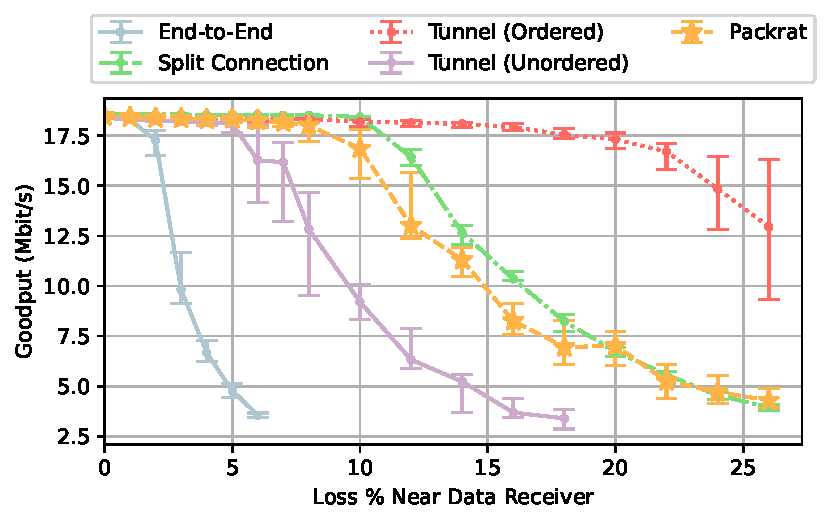
\includegraphics[width=\linewidth]{packrat-paper/figures/http_benchmark.pdf}
        \caption{QUIC HTTP/3 file download.}
        \label{fig:perf:http}
    \end{subfigure}
    \begin{subfigure}[b]{\linewidth}
        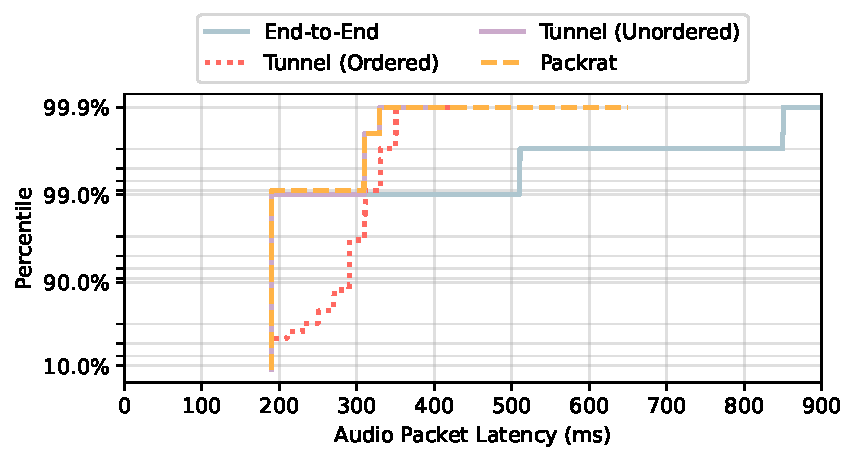
\includegraphics[width=\linewidth]{packrat-paper/figures/media_benchmark.pdf}
        \caption{Low-latency media stream with FEC.}
        \label{fig:perf:media}
    \end{subfigure}
    \begin{subfigure}[b]{\linewidth}
        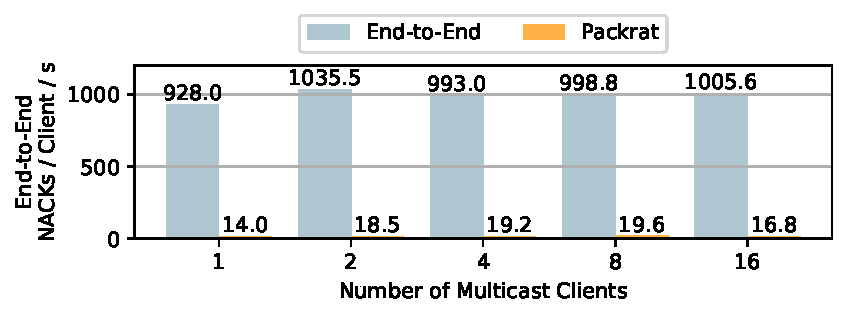
\includegraphics[width=\linewidth]{packrat-paper/figures/multicast_benchmark.pdf}
        \caption{Reliable IP multicast stream.}
        \label{fig:perf:multicast}
    \end{subfigure}
    \vspace{-0.3cm}
    \caption{The Packrat protocol achieves better throughput, latency, and link
     overheads in lossy network settings compared to end-to-end
     retransmissions. Applications using the tunnel differ in how much they
     benefit based on the tunnel configuration, which is a disadvantage of
     link-layer retransmissions.}
    \label{fig:perf}
\end{figure}

For the HTTP/3 download in this low-latency, low-loss network setting, the
ordered tunnel outperforms QUIC with a Packrat. The unordered tunnel does not
perform as well because the retransmits at millisecond timesecales arrive
out-of-order. The end-to-end ACKs subsequently cause the server to send
spurious retransmissions (\Cref{fig:http:spurious}). The congestion response to
spurious retransmissions is not well-defined in standards, and \texttt
{picoquic} makes some attempt to revert the congestion window that leads to
this result, which is a similar result we observe when using Packrat with no
reorder signal. The ordered tunnel does not run into the same issues because
its aggressive retransmissions, when ordered, hide most loss the server could
interpret as a congestion signal.

\paragraph{Low-latency media with FEC.}

Packrat enables fewer and shorter stalls in a low-latency media stream over a
high-delay satellite network (\Cref{fig:perf:media}). In this network setting,
the minimum one-way latency of a packet is already 190 ms (40 ms encoding + 150
ms delay). For reference, 150 ms is the normal latency for VoIP, and anything
above produces a noticeable drop in quality. Thus network-generated
retransmissions are crucial in lossy, high-latency settings.

Both Packrat and end-to-end benefit from FEC, but Packrat enables shorter stalls when
a frame still needs to be retransmitted. In this transport protocol, a frame
needs to be retransmitted if two packets are lost in a row. Thus at 10\% loss,
the 99th percentile delay of both mechanisms is the minimum of 190 ms. In the
remaining percentile, one more out-of-order packet arrives after $20$ ms,
draining the last of the buffer and generating an eACK or NACK. The length of
the stall is then the 100 or 300 ms RTT with the proxy or server. The unordered
tunnel exhibits a similar behavior to Packrat.

Unlike the HTTP/3 benchmark, this transport protocol gets none of the benefits
of FEC with the \textit{ordered} tunnel. When a retransmission is required, the
tunnel buffers at least 6 more packets until it receives the retransmission and
releases them to the client. The buffering causes unnecessary stalls. If the
tunnel had just released the packets, a single missing packet would have been
masked by the repetition code.

\paragraph{Reliable IP multicast stream.}

Caching packets in the network like a CDN is inherently beneficial because it
can reduce the congestion in the core network. This is one of the idealistic
draws of IP multicast, but it is rarely used over the Internet in practice
because a reliable stream may require an overwhelming number of unicast
retransmissions from the server when there is loss. While CDNs and SFUs have
helped with content distribution, these are not options for encrypted transport
protocols without embedding trust in the network.

The Packrat proxy can handle in-network retransmissions for a large number of
multicast clients. Each client using the Packrat protocol sends on average $16.8$
end-to-end retransmissions/second, a $59\!\times$ reduction from $1005.6$
retransmissions/second/client without Packrat. This reduction scales with the
number of clients. In-network retransmissions reduce both the load at the
server and congestion in the network.\\

\noindent
The behaviors of the QUIC and media transport protocols with various tunnels
represent the challenges of configuring link-layer retransmissions
independently of the applications that share the link. A large download
over QUIC performs poorly
when there is excessive reordering, while the media transport protocol prefers
to receive packets right away.
Disabling link-layer retransmissions introduces loss, which can be even more
detrimental for performance.

\subsection{Link Overheads}
\begin{figure*}[ht]
\centering
\begin{minipage}[t]{0.3\textwidth}
    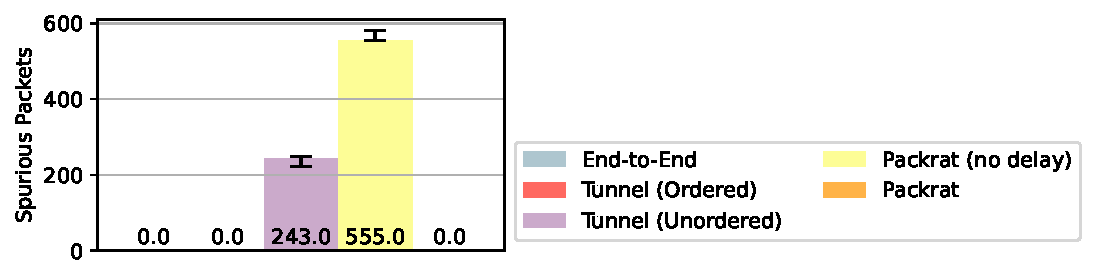
\includegraphics[width=\linewidth, trim=245 15 5 65, clip]{packrat-paper/figures/spurious_retx_legend.pdf}
    \begin{subfigure}[b]{\linewidth}
        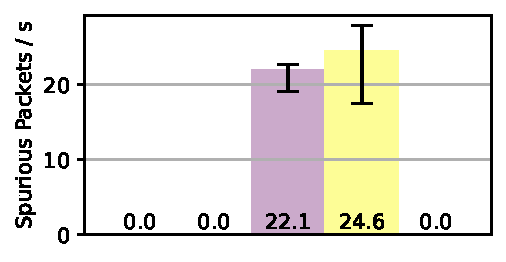
\includegraphics[width=\linewidth]{packrat-paper/figures/spurious_retx_http.pdf}
        \caption{HTTP/3 download.}
        \label{fig:http:spurious}
    \end{subfigure}
    \begin{subfigure}[b]{\linewidth}
        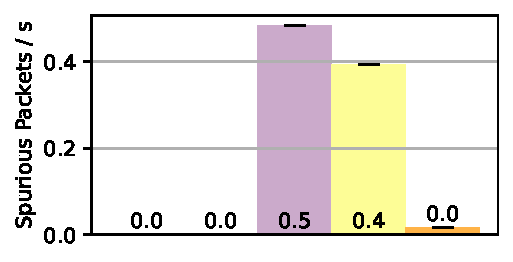
\includegraphics[width=\linewidth]{packrat-paper/figures/spurious_retx_media.pdf}
        \caption{Low-latency media.}
        \label{fig:media:spurious}
    \end{subfigure}
    \caption{The unordered tunnel and Packrat without modifying the end-to-end
     reorder signal cause the client to receive spurious retransmissions.
     Modifying the end-to-end signal with Packrat significantly reduces them.}
    \label{fig:spurious}
\end{minipage}%
\hfill
\begin{minipage}[t]{0.68\textwidth}
    \centering
    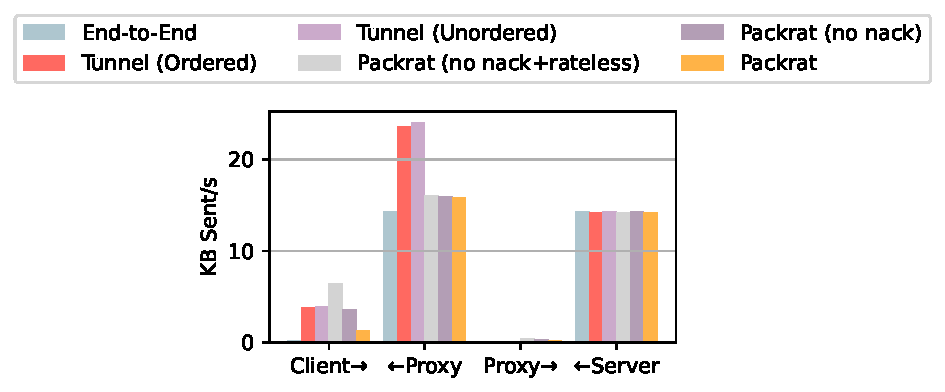
\includegraphics[width=0.9\linewidth, trim=5 140 5 5, clip]{packrat-paper/figures/network_stats_media_legend.pdf}
    % 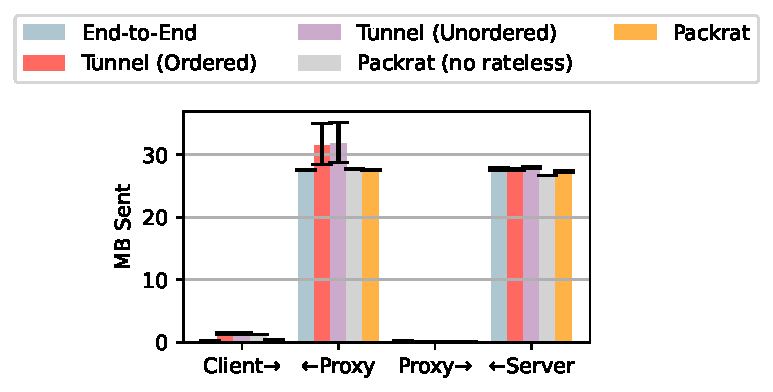
\includegraphics[width=0.7\linewidth, trim=5 140 5 5, clip]{packrat-paper/figures/network_stats_http_legend.pdf}
    
    \begin{subfigure}[b]{0.48\linewidth}
        \centering
        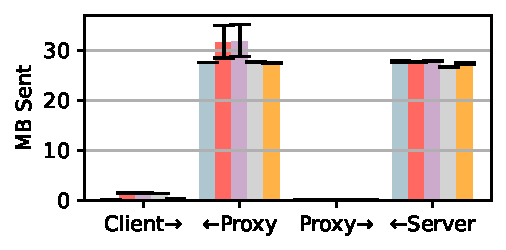
\includegraphics[width=\linewidth]{packrat-paper/figures/network_stats_http_tx_bytes.pdf}
        \caption{HTTP/3 download (bytes).}
        \label{fig:link-overheads:http-bytes}
    \end{subfigure}
    \begin{subfigure}[b]{0.51\linewidth}
        \centering
        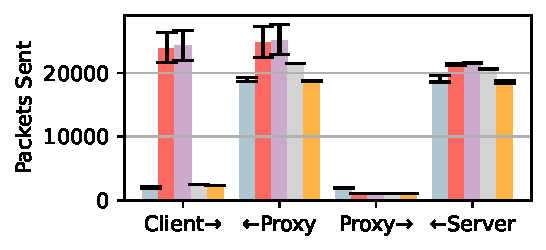
\includegraphics[width=\linewidth]{packrat-paper/figures/network_stats_http_tx_packets.pdf}
        \caption{HTTP/3 download (packets).}
        \label{fig:link-overheads:http-packets}
    \end{subfigure}\\

    \begin{subfigure}[b]{0.49\linewidth}
        \centering
        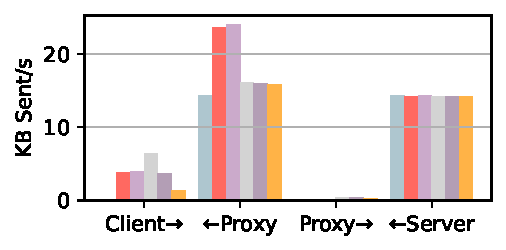
\includegraphics[width=\linewidth]{packrat-paper/figures/network_stats_media_tx_bytes.pdf}
        \caption{Low-latency media (bytes).}
        \label{fig:link-overheads:media-bytes}
    \end{subfigure}
    \begin{subfigure}[b]{0.49\linewidth}
        \centering
        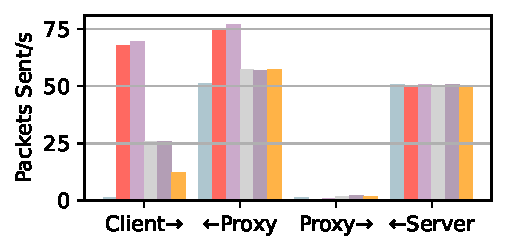
\includegraphics[width=\linewidth]{packrat-paper/figures/network_stats_media_tx_packets.pdf}
        \caption{Low-latency media (packets).}
        \label{fig:link-overheads:media-packets}
    \end{subfigure}
    
    \caption{The number of bytes (left) and packets (right) sent between the
     client, proxy, and server. The statistics are captured directly from the
     network interface. The link overheads from quACKs in the Packrat protocol are
     comparable to those of the underlying acknowledgment scheme. The client
     sends fewer bytes with rateless quACKs, and fewer packets when it
     selectively quACKs. The tunnel aggressively ACKs and retransmits.}
    \label{fig:link-overheads}
\end{minipage}
\end{figure*}

In this section, we analyze how sending eACKs with the optimizations in \Cref
{sec:eack:hints} impacts the link overheads in the network.
\Cref{fig:link-overheads} displays the number of packets and bytes sent on each
link between the client, proxy, and server in the HTTP and media applications.
As a proportion of the volume in bytes sent by both endpoints of the
application, the HTTP client makes up $1.3\%$ of the traffic with Packrat and
$0.7\%$ without. The media client makes up $8.2\%$ of the traffic with Packrat
and $1.0\%$ without. We find that that we can reasonably think of eACKs as
control packets in the common case.

\paragraph{Rateless eACKs.}
Using the rateless property to send smaller eACKs
reduces the number of bytes the client sends by $3.6\!\times$ (\Cref
{fig:link-overheads:http-bytes}) and $1.8\!\times$ (\Cref
{fig:link-overheads:media-bytes}) compared to Packrat without the optimization.
% http sender tx_bytes 1266149.5 -> 351208.0
% 1266149.5/351208.0=3.6x
% media sender tx_bytes 6397.578993802214 -> 3632.7542920194414 -> 1.8x
This property allows clients to configure the number of symbols less
conservatively when initializing the Packrat connection while being able to
dynamically adjust to changing loss conditions, particularly in less controlled
non-emulation environments.

\paragraph{Sending eACKs on NACK.}

% media sender tx_packets 25.786554138093248 -> 12.33599987063784
Sending a eACK only when the client would otherwise send a NACK reduces the
number of packets the media client sends $1.9\!\times$ (\Cref
{fig:link-overheads:media-packets}). Note that without sending on NACK, we
configured the media client to eACK every other packet to balance latency with
frequent eACKing. The media client sends more packets than end-to-end because
although it only ACKs when there is a missing \textit{frame}, it eACKs when
there is a missing \textit{packet} because the FEC is opaque to the proxy.
% media sender tx_bytes 1275.1961129433735 -> 147.66572118181435
% 1127.53 * 8 = 9 Kbit

\paragraph{Base connection improvements.}

Even though the HTTP client eACKs at a similar frequency to which it ACKs, the
client sends a similar number of packets with and without the Packrat (\Cref
{fig:link-overheads:http-packets}). The proxy in the end-to-end scenario sends
nearly twice as many ACKs to the server because the number of ACKs depends on
the length of the connection. Packrat improves the throughput so much that the
number of net packets sent by the client are similar.

The IP multicast application demonstrates how Packrat can reduce congestion closer
to the server by caching retransmissions in the middle of the network (\Cref
{fig:perf:multicast}). This is especially impactful if the data is shared by
multiple clients.\\

\noindent Note that the tunnels aggressively ACK and retransmit in both
directions. The client sends $12$-$66\!\times$ additional packets compared to
end-to-end and the proxy sends $33$-$51$\% more to the client. Even though the
block ACKs are small, it can be costly for radios to switch often between
sending and receiving modes, and for proxies with per-packet overheads.

\subsection{CPU Overheads}

In this experiment, we analyze the number of cycles that the proxy
needs to process each
packet in the HTTP/3 benchmark, and use the per-packet overheads to
extrapolate the capacity of a CPU-constrained proxy. These overheads
include both eACK operations and transport-protocol logic for e.g.,
packet triaging, loss detection, and cache management.

Each data packet on the base connection takes on average $1002$ cycles/packet.
The main overhead comes from adding the packet to a ring buffer used as the
packet cache.

Each eACK on the Packrat connection takes on average 27716 cycles/packet. The
proxy determines which packets to retransmit based on the eACK and evicts
packets. Loss detection involves encoding a delta of packets since the last
eACK into the existing state, as well as decoding the received eACK. Encoding
uses a total of $7156/27716 = 25.8\%$ of the cycles and decoding $3560/27716 =
12.8\%$. With a total of $38.6\%$ of the processing time spent on IBLT
operations, this implies that encoding and decoding are valuable to optimize.

% psum
% WARN [proxy::cycles] transport
% WARN [proxy::cycles] 953 (total=101000,prop=1.000)
% WARN [proxy::cycles] transport,encode,decode
% WARN [proxy::cycles] 32923,9572,2984 (total=6800,prop=1.000,1.000,0.789)

% iblt
% WARN [proxy::cycles] transport
% WARN [proxy::cycles] 1002 (total=101000,prop=1.000)
% WARN [proxy::cycles] transport,encode,decode
% WARN [proxy::cycles] 27716,7156,3560 (total=6200,prop=1.000,1.000,0.516)

In this application, there is approximately one eACK for every $16.3$ data
packets. If each data packet uses a full MTU of 1500 bytes, this means a single
core of a 2.4 GHz CPU on a proxy would theoretically be able to handle 10.7
Gbit/s\footnote{ $2.4\text{ Gcycles/s }
\times(16.3 \text{ data packets } / (27716\cdot1 + 1002\cdot16.3) \text{ cycles })
\times (1500 \text{ bytes/data packet })
\times (8 \text{ bits/byte })
= 10.7 \text{ Gbit/s}$.
}. However, this estimate does not account for the substantial CPU overhead
involved in reading and writing to the NIC---these can be significantly reduced
using kernel bypass frameworks like DPDK or with specialized networking
hardware.

% iblt
% 2.4 Gcycles/s
% * 16.29 data packets / (27716*1 + 1002*16.29) cycles
% * 1500 bytes / data packet
% * 8 bits / 1 byte
% = 10.7 Gbit/s.

% psum
% 2.4 Gcycles/s
% * 14.85 data packets / (32923*1 + 953*14.85) cycles
% * 1500 bytes / data packet
% * 8 bits / 1 byte
% = 11.2 Gbit/s

\subsection{Memory Overheads}

\begin{figure}[t]
    \centering
    \begin{subfigure}[b]{0.8\linewidth}
        \centering
        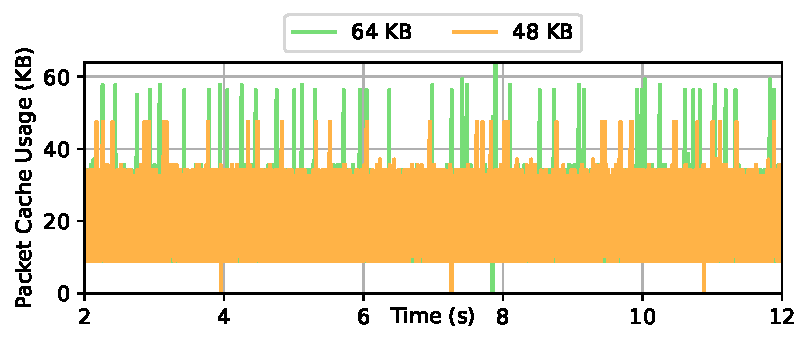
\includegraphics[width=\linewidth]{packrat-paper/figures/cache_http.pdf}
        \caption{HTTP/3 file download.
        % \thea{May be a non-issue, but not sure how to interpret the mass of orange here.}
        }
        \label{fig:memory:http}
    \end{subfigure}
    \begin{subfigure}[b]{0.8\linewidth}
        \centering
        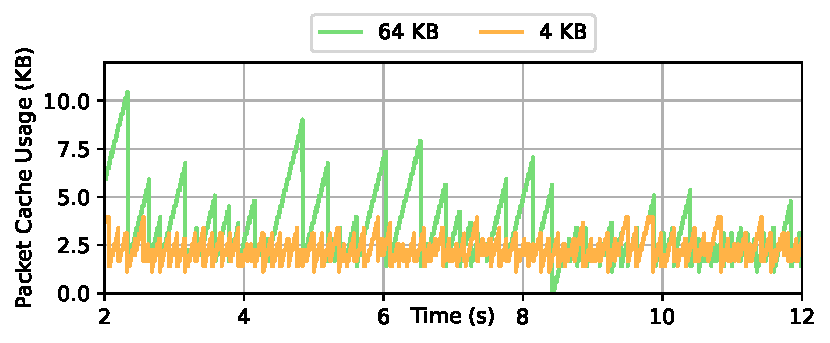
\includegraphics[width=\linewidth]{packrat-paper/figures/cache_media.pdf}
        \caption{Low-latency media with FEC.}
        \label{fig:memory:media}
    \end{subfigure}
    \caption{\small The number of bytes in the cache over a
     10-second period with both bounded (48 KB or 4 KB) and unbounded (64 KB)
     cache sizes. The proxy uses optimistic eviction if an incoming packet
     causes the cache to exceed its capacity.}
    \label{fig:memory}
\end{figure}

\begin{figure}[t]
    \centering
    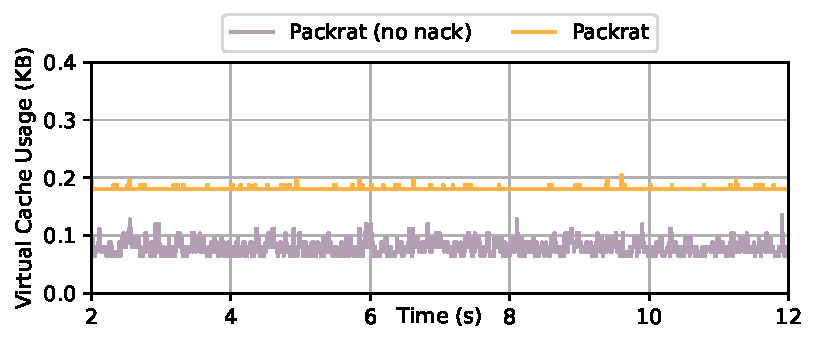
\includegraphics[width=0.8\linewidth]{packrat-paper/figures/cache_multicast.pdf}
    \caption{The sum of the virtual cache sizes of all $16$ clients in
     the multicast application. Each client uses $\approx\!$12 bytes each for a
     single insertion pair. The variations are due to individuals having
     slightly more or less than one insertion pair. Without selective quACKing
     (``no nack''), clients more often have empty virtual buffers. The base
     connection's packet cache (not pictured) is always 64 KB.}
    \label{fig:memory:multicast}
\end{figure}

We find that the Packrat proxy needs no more memory
than similar proxies for unencrypted transport protocols, and that the optimistic
eviction policy is an effective fallback for when the cache exceeds its memory limits.
Like any in-network retransmission mechanism,
the most significant memory usage at the proxy comes from the packet
cache. \Cref{fig:memory} shows the number of bytes in the packet contents of
the cache over a 10-second period of each application in our chosen
network settings. The maximum cache size
at the Packrat proxy is 64kB per connection, similar to a typical TCP window size.

\paragraph{HTTP/3 file download.}

The cache grows quickly because each data packet is large, but evicts
packets every 10~ms when
it receives an eACK (\Cref{fig:memory:http}). The minimum cache size is
$\approx\!10$ kB, the size of the outstanding packets between the client and
proxy. A spike occurs when an eACK is dropped, at which point the proxy
optimistically evicts. The proxy resets the connection if there is an
error, which is more common with a smaller cache, and drops the cache
size to 0.

\paragraph{Low-latency media with FEC.}

The media application relies on optimistic eviction to keep the cache small
since the client selectively eACKs (\Cref{fig:memory:media}). The
line plateaus at the maximum cache size because the proxy
assumes these packets have been received. The cache size only needs to fit 1-2
RTTs of packets between the client and proxy.

\paragraph{Reliable IP multicast stream.}

The multicast application has a fixed packet cache size of 64 kB, and we analyze
the memory overheads of the per-client virtual caches (\Cref
{fig:memory:multicast}). In particular, we calculate the overhead of each
virtual cache as 4 bytes for the first global index and then 8 bytes for each
insertion pair (\Cref{sec:implementation:proxy}). When there are 16 clients,
the proxy uses on average 0.178 KB in the virtual caches for a very low
overhead of 12 bytes/client. That is exactly one insertion pair, and in general
the overheads of the virtual caches are proportional to the number of
outstanding retransmissions.
% average = 0.17788111888111888 KB = 1

\chapter{Split Throughput Heuristic}
\label{sec:splitting}

\begin{figure}[t!]
    \centering
    \begin{subfigure}[b]{\linewidth}
        \centering
        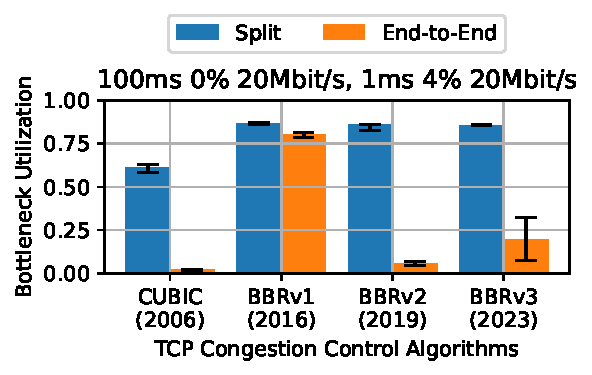
\includegraphics[width=0.8\linewidth]
         {splitting-paper/figures/bbr_over_time/bbr_over_time_network_20_20_100_1_None_None_0_4.pdf}
        \captionsetup{skip=0pt}
        \caption{Asymmetric, lossy last-mile.}
        \label{fig:bbr-over-time:class1}
    \end{subfigure}
    \begin{subfigure}[b]{\linewidth}
        \centering
        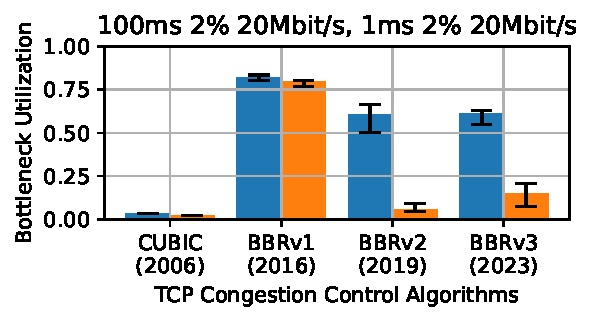
\includegraphics[width=0.8\linewidth]
         {splitting-paper/figures/bbr_over_time/bbr_over_time_network_20_20_100_1_None_None_2_2.pdf}
        \captionsetup{skip=0pt}
        \caption{Asymmetric, both path segments are lossy.}
        \label{fig:bbr-over-time:class2}
    \end{subfigure}
    \begin{subfigure}[b]{\linewidth}
        \centering
        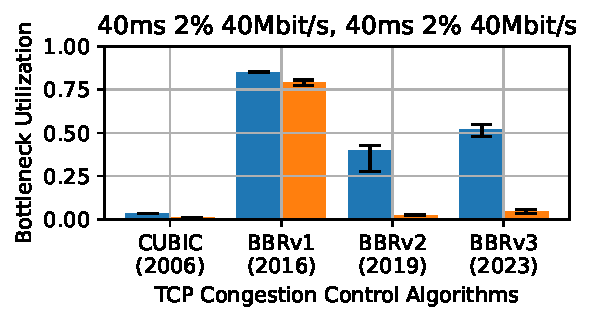
\includegraphics[width=0.8\linewidth]
         {splitting-paper/figures/bbr_over_time/bbr_over_time_network_40_40_40_40_None_None_2_2.pdf}
        \captionsetup{skip=0pt}
        \caption{Symmetric, both path segments are lossy.}
        \label{fig:bbr-over-time:class3}
    \end{subfigure}
    \caption{\small Three classes of network settings in which the throughput of a
     long-lived data transfer using BBRv3 benefits significantly from
     connection-splitting. While the throughput of TCP using BBRv1 may not have
     benefitted from a PEP, as the BBR algorithm has evolved over time, it has
     also made connection-splitting pertinent again. In two of these classes,
     split BBRv3 even achieves high bottleneck link rate utilization where split
     CUBIC does not. IQR of $n=20$.}
    \label{fig:bbr-over-time}
\end{figure}


A stylized history of connection-splitting over the Internet could go
roughly as follows: In the 1970s, TCP was designed as a host-to-host
transport for flow-controlled reliable byte streams. In the late
1980s, TCP implementations added congestion control~\cite{vjk} to
respond to network-path limitations and contention, with indications
of packet loss as the primary congestion signals. As Internet use
exploded in the 1990s, it became apparent that contemporary TCP
implementations performed poorly over long paths with packet loss. By
the late 1990s, many network operators deployed commercial ``TCP
accelerators,'' also known as ``performance-enhancing proxies''
\cite{rfc3135, honda2011still}, to improve customers' TCP
throughput. These proxies transparently split a TCP connection in two,
providing an intermediate point of acknowledgment and retransmission
and transforming an end-to-end TCP connection into two independent
connections.

PEPs were marketed as improving users' throughput, especially where a
PEP splits a high-delay, lossy path into two segments, each with less
delay or less loss. Past surveys found connection-splitting PEPs
deployed on large numbers of wireless and satellite
networks~\cite{rfc3135, honda2011still}. But for almost as long as
these PEPs have existed, purists have criticized their alleged
benefits as exaggerated or unfair, sensitive to the details of an
endpoint's congestion-control scheme, contrary to end-to-end
arguments~\cite{saltzer1984endtoend}, and likely to lead to
ossificiation~\cite{papastergiou2017deossifying, edeline2019bottomup}.

Two more-recent developments have put PEPs on the back foot. The QUIC
transport protocol, standardized in 2021~\cite{rfc9000}, is encrypted
end-to-end and, unlike TCP, its connections can't be split by a
transparent proxy---but its wide deployment by major traffic sources (particularly Google)
in the 2010s didn't produce a measured reduction in performance,
compared with TCP connections that do benefit from PEPs in the
field~\cite{langley2017quic}. If PEPs had really been aiding TCP connections all this time,
QUIC could have been expected to experience lower sustained throughput
over such paths (compared with TCP connections between the same
endpoints, using the same congestion-control schemes).

Furthermore, the BBR congestion-control scheme~\cite{cardwell2017bbr}, first
released in 2016, now controls a large percentage of Internet traffic
(both TCP and QUIC)~\cite{ware2024ccanalyzer} and puts less emphasis on packet
loss as a congestion signal than older schemes in wide
deployment, such as CUBIC. Because much of PEPs' benefit comes from
splitting up long, lossy paths for the benefit of ``loss-based''
schemes, it has been suggested that BBR has led to
a sharp decline in the use of PEPs~\cite{frode}.

\textbf{Do BBR and QUIC make connection-splitting obsolete?} In this
paper, we present findings that suggest that neither of these
developments should be regarded as reliable;
Connection-splitting may yet play a performance-enhancing role
on the Internet, despite its controversial nature.

We conduct a measurement study in emulation to investigate what kinds of
congestion control schemes, network scenarios, and transport protocols may
still experience increased sustained throughput from connection-splitting. We
aid our analysis with a \textit{split throughput heuristic} for predicting the
throughput of a split
connection, based on the measured end-to-end throughput of each segment on the
split path. We aim to (1) explore a wide parameter space of network settings
and congestion control schemes and (2) reason about encrypted transport
protocols (QUIC) that we cannot directly measure.

We present three major findings:

\paragraph{Finding 1: Splitting has become significantly more beneficial to TCP
 BBR since it was initially released in 2016.}

We confirm that BBR's initial ``v1'' release does not benefit markedly from splitting, unlike earlier
congestion-control schemes. But as the BBR algorithm
has evolved into BBRv2 in 2019 and now BBRv3 in 2023, it has also evolved to
behave more conventionally in the sense that it benefits from being
split---just like more traditional, loss-based congestion control schemes such
as CUBIC (\Cref{fig:bbr-over-time}).

The regression in split throughput follows directly from the regression
in end-to-end throughput, via the heuristic. While BBRv1 nearly always achieves
full utilization, BBRv3 sees lower utilization in lossy
settings, leaving more to gain from splitting.
The end-to-end regression is because BBRv3 has increased its loss sensitivity
to coexist fairly with ``loss-based'' schemes such as Reno and
CUBIC~\cite{cardwell2024bbrv3-ietf119,ware2019modeling,zeynali2024promises}.
Thus, we find that BBR and its split behavior continue
to evolve, and that the model-based BBR algorithm has \textit{not} made the
performance enhancements of connection-splitting obsolete.

\paragraph{Finding 2: There exist classes of network paths where TCP BBR would
 significantly benefit from splitting but TCP CUBIC would not.}

Splitting not only benefits BBRv3 in all the same scenarios as CUBIC (in terms
of long-lived throughput), it also benefits BBRv3 in \textit{new} scenarios. In
particular, there exist classes of network settings where the CCA achieves a
very low bottleneck link rate utilization \textit{without} a PEP, but a high
bottleneck link rate utilization \textit{with} a PEP.

More specifically, in addition to edge deployments with a lossy last-mile (\Cref
{fig:bbr-over-time:class1}), BBRv3 can also benefit from splitting in
scenarios where there is loss on both path segments (\Cref
{fig:bbr-over-time:class2}), and when the connection-splitter is located
farther from the edge (\Cref{fig:bbr-over-time:class3}). This suggests that in
these network classes, simple split BBRv3 can replace the
proprietary protocols that have traditionally been used to address middle-mile
loss, particularly in satellite and wireless ad-hoc networks~\cite
{cloudsplitting2010,border2020evaluating,rfc3135}. We should continue to
evaluate the behavior of split CCAs in new types of networks, especially in
space.

\paragraph{Finding 3: Implementations of the ``same'' congestion-control schemes
in QUIC vary significantly, and further differ those of Linux TCP---frustrating
attempts to directly compare performance between QUIC and TCP.}

In an initial study of three QUIC implementations, we find that the end-to-end
behaviors of the same congestion control schemes vary significantly by implementation.
The implementations vary in both baseline performance and sensitivity to loss
and delay. By applying the split throughput heuristic, we find that some
CUBIC implementations can actually benefit in the same classes of network paths
as TCP BBRv3. We also find that BBR is challenging to implement, with various
BBRv3 implementations exhibiting non-uniform end-to-end behavior and thus no
clear trend in split behavior. We argue that the benefits of in-network
assistance should be considered along with not just a CCA, but their specific
implementations. \\

\noindent Our initial evaluation suggests that the performance improvements of
connection-splitting remain relevant in the context of today's model-based
congestion control algorithms, encrypted transport protocols, and satellite and
wireless ad-hoc network settings. As congestion-control schemes continue to
evolve, we urge researchers to refer to them by
algorithm/implementation/version, not just ``BBR'' or even ``QUIC BBRv1''. We
urge the community to create a performance test suite for an implementation to
be able to claim that it conforms to a particular congestion-control standard.
Finally, we hope that this work motivates the community to pursue
protocol-agnostic PEPs that achieve the performance benefits of in-network
assistance without the ossification downsides.

\section{Background: BBR and QUIC}
\label{sec:splitting:background}

In this section, we provide additional context on some concepts that we refer to
throughout the text.

\paragraph{Performance-enhancing proxies.}

The idea of in-network assistance has long brought pain to the hearts of
Internet researchers, protocol designers, and network operators. In particular,
the word ``middleboxes'' is often associated with NATs, firewalls, and other
policy enforcers that modify or inspect data in ways that break end-to-end
behavior. A substantial percentage of Internet paths are affected by feature or
protocol-breaking policies of middleboxes~\cite{edeline2019bottomup}.

In contrast, we refer specifically to the type of assistance provided by
performance-enhancing ``proxies'', or PEPs, that transparently split a TCP
connection in two~\cite{rfc3135}. While PEPs still interfere with end-to-end
transport mechanisms, their goal is to enhance the user experience by
maximizing performance, as opposed to enforce security or routing policies.

Connection-splitting PEPs can enhance performance in several ways. By providing
an intermediate point of acknowledgment and retransmission, PEPs reduce the
length of the feedback loop for signals of loss and congestion. The PEP also
allows each side of the split connection to better optimize congestion control
and flow control for network conditions local to the path segment. We can
expect PEPs to impact a variety of performance metrics, including startup time,
packet jitter, retransmission overheads, and more. In this paper, we focus
only on the impact of connection-splitting on the \textit{sustained throughput}
of long-lived data transfers.

\paragraph{Congestion control.}

Congestion control was originally deployed in the 1980s to manage the explosive
growth of the Internet~\cite{vjk}. Foundational algorithms such as slow start
and fast retransmit eventually became part of the Tahoe congestion control
scheme. Variants such as NewReno and CUBIC emerged over time to improve
performance with fairness~\cite{ha2008cubic}. CUBIC is the default congestion control module for
TCP in the Linux kernel, and widely deployed. It is the primary ``loss-based''
congestion control scheme that we evaluate.

The word ``TCP'' is sometimes used synonomously with the congestion control
algorithms that it implements. In reality, the two are distinct, though deeply
intertwined. For example, the QUIC transport protocol implements many of the
same algorithms as TCP to manage network traffic, even though it runs over UDP~\cite{rfc9000}.
In this paper, we refer to ``TCP'' and ``QUIC'' as the transport protocols,
``Linux TCP'' as the implementation of TCP in the Linux kernel, and congestion
control schemes as the particular manifestations of a congestion control
algorithm in a transport protocol implementation.

\paragraph{BBR.}

Today, the focus on congestion control has shifted towards BBR. BBR is sometimes
referred to as a ``model-based'' congestion control scheme because it relies on
a fundamentally different approach of modeling network bandwidth and round-trip
time. It does not use packet loss as the primary signal for congestion. Google
initially presented BBR in 2016 as addressing the problems of CUBIC in
high-speed networks~\cite{cardwell2016bbr-ietf97}.

Over time, BBR encountered controversy for its unfairness towards loss-based
schemes~\cite{ware2019modeling,philip2021revisiting,cao2019use}. In response,
``v1'' of BBR has now evolved into BBRv2 in 2019 and BBRv3 in 2023, driven by
efforts at Google. Today, Google recommends that BBRv1 and BBRv2 be
deprecated in favor of BBRv3~\cite{cardwell2024bbrv3-ietf119}.

BBR is also widely deployed~\cite
{cardwell2024bbrv3-ietf119-qna,ware2024ccanalyzer}. Google has contributed BBR
implementations to the Linux kernel, and Amazon, Akamai, Meta, and Cloudflare
CDNs all use BBRv1 for TCP. At Google, BBRv3 is used in all google.com and
YouTube public Internet traffic with TCP, and is currently being A/B tested
against BBRv1 in Google QUIC traffic~\cite{cardwell2024bbrv3-ietf119}.
It is estimated that 40\% of traffic used BBR in 2019~\cite{mishra2019great}.

% https://datatracker.ietf.org/doc/draft-cardwell-ccwg-bbr/history/
Since 2017, there have been ongoing efforts to standardize BBR in the IETF~\cite{cardwell2024bbr-ietf-draft}.
However, progress has been slow. The Internet draft goes years or months at a
time without an update at the mercy of Google contributors. While companies
have been quick to adopt BBR in Linux TCP, adoption in QUIC has been slower.
Anecdotally, some have resorted to reverse engineering the Linux
implementation, and some such as Cloudflare, Meta, and Cisco are actively
experimenting with variants of BBRv2+ in their QUIC stacks~\cite
{cardwell2024bbrv3-ietf119-qna}.

\paragraph{QUIC.}

The QUIC transport protocol was originally developed by Google in 2012 to
improve performance for HTTPS traffic and to enable the rapid
evolution of transport mechanisms. QUIC is implemented over UDP, and moves
congestion control development from kernel space to user space.

As of 2021, QUIC is now a standards-track RFC~\cite{rfc9000} with widespread
deployment and interoperability testing~\cite{quic-interop}. It is estimated
that 8.4\% of global websites support QUIC~\cite{w3techs}, many of them major
traffic sources such as Cloudflare.
Still, many high-speed flows remain on TCP due to better TCP hardware
capabilities and ``per-origin'' caching, which complicates multi-CDN
deployments that mix protocols.

Evaluations of QUIC at the Internet scale generally show improved performance
compared to TCP, except in satellite networks. Features like zero-RTT
connection establishment and stream multiplexing enable measured improvements
in search latency, rebuffer rate, and other video playback metrics at
Google~\cite{langley2017quic}. Satellite network operators, on the other hand,
experience strife when it comes to QUIC. Several studies have measured the
negative impact of encryption on performance in split satellite
environments~\cite
{kosek2022quicpep,martin2022suitability,kuhn2021quic-over-sat,border2020evaluating}.

\section{Split Throughput Heuristic}
\label{sec:splitting:heuristic}

When initially considering which network scenarios to evaluate in our emulation
study, we discovered it to be non-trivial to pick scenarios that would lead to
a general understanding of the throughput of a congestion control scheme in a
split setting. It is challenging to select which network settings and
combinations of path segments to evaluate, as the parameter space for
combinations of path segments can be quite large. Also, not all CCA
implementations can be trivially split.

For this paper, we refer to \textit{throughput} as the throughput of a
long-lived data transfer in an emulated network, using a single flow.
We do not evaluate other metrics such as startup time, retransmission
overheads, or short-lived data transfers, which have been of interest to
PEPs and could also be impacted by connection-splitting.
When discussing throughput, we refer to \textit{end-to-end throughput} as
the throughput of an end-to-end connection, and \textit{split throughput} as the
throughput of the same connection when there is a connection-splitting PEP.

We realized that while split throughput is not necessarily well
understood for any combination of CCA, transport protocol, and network setting,
the end-to-end throughput often \textit{is}. We make the following insight
based on an ideal setting:

\begin{figure}[h]
  \centering
  \begin{tcolorbox}[colback=yellow!20, width=\linewidth, sharp corners]
    \textbf{Split Throughput Heuristic:} We can estimate the long-lived ``split
     throughput'' of a connection by measuring the long-lived ``end-to-end
     throughput'' on each segment of the split path and taking the minimum.
  \end{tcolorbox}
  \caption{\small A heuristic for evaluating split behavior from end-to-end behavior in
   an emulated network.}
  \label{fig:heuristic}
\end{figure}

\noindent Thus if we know the throughput of the much smaller parameter
 space of end-to-end connections, we can easily derive:

\begin{enumerate}[noitemsep]
    \item The split throughput of a CCA on a network path composed of two path
     segments,
    \item The end-to-end throughput on the network path,
    \item The expected throughput benefit of using a connection-splitting PEP
     on the network path.
\end{enumerate}

Furthermore, it is impossible to quantitatively evaluate the split throughput
of encrypted transport protocols without creating a custom and explicit
connection-splitting PEP. As a result, it is challenging to establish a
baseline for the throughput that is potentially achievable by QUIC with
in-network assistance, leaving many studies to compare QUIC only to split TCP~\cite
{thomas2019google,border2020evaluating,yuan2024sidekick}. The split throughput
heuristic allows us to estimate the throughput of encrypted transport
protocols using knowledge about its end-to-end throughput, without
actually splitting the connection.

In \Cref{sec:splitting:accuracy}, we discuss potential sources of error in the heuristic,
including the lack of consideration of the queue configuration on the proxy
or the placement of the bottleneck link relative to the data sender. However,
we believe there is a design tradeoff in accuracy versus simplicity.

In the rest of this section, we first describe how to use this heuristic to
analyze the split throughput benefit in a single network setting, without
having to run an emulation with a connection splitter. Then we describe how we
cache emulation results for an end-to-end parameter space to enable a more
open-ended analysis of CCAs over a variety of networks. Finally, we discuss the
limitations of our methodology using the heuristic, and propose possible
extensions.

\subsection{Example Usage in a Single Network Setting}
\label{sec:splitting:heuristic:example}

\begin{lstfloat}[t]
\begin{lstlisting}[language=Python]
class NetworkModel:
    def __init__(self, delay, bw, loss):
        self.delay = delay
        self.bw = bw
        self.loss = loss

def compose(s1: NetworkModel,
            s2: NetworkModel) -> NetworkModel:
    delay = s1.delay + s2.delay
    bw = min(s1.bw, s2.bw)
    loss = s1.loss * (1-s1.loss)*s2.loss
    return NetworkModel(delay, bw, loss)

def throughput(s: NetworkModel) -> float:
    return run_emulation(s)
\end{lstlisting}
\captionof{lstlisting}{\small An interface for modeling a network path and estimating
 throughput. The \texttt{compose()} function models an end-to-end network path
 from two path segments. The \texttt{throughput()} function obtains a throughput
 measurement for a path segment.}
\label{lst:multi-segment-network-model}
\end{lstfloat}

\begin{lstfloat}[t]
\begin{lstlisting}[language=Python]
def pred_split_throughput(s1: NetworkModel,
                          s2: NetworkModel) -> float:
    return min(throughput(s1), throughput(s2))

def pred_e2e_throughput(s1: NetworkModel,
                        s2: NetworkModel) -> float:
    s = compose(s1, s2)
    return throughput(s)
\end{lstlisting}
\captionof{lstlisting}{\small Functions that apply our simplified network model and the
 split throughput heuristic (\Cref{fig:heuristic}) to predict split and
 end-to-end throughput, using the interface in \Cref
 {lst:multi-segment-network-model}.}
\label{lst:pred-throughput-api}
\end{lstfloat}

Given a network model of the two path segments that compose an end-to-end
network path, we would like to be able to estimate the expected throughput
benefit of using a connection-splitting PEP between the two segments. In our
emulation study, our simplified network model consists of three
parameters: delay, bandwidth, and loss.

We explicitly define the interface we
use to query split and end-to-end throughput in \Cref
{lst:multi-segment-network-model,lst:pred-throughput-api}. In addition
to the network model, we implement functions to \texttt{compose()} a model of
an end-to-end network path from two path segments and to
query the end-to-end \texttt{throughput()} of a segment.

\paragraph{The \texttt{compose()} function.}
Since our network model consists of three parameters, we describe how to compose
each of these parameters to model the end-to-end network path. Bandwidth is the
minimum of the two bandwidths, which is the bottleneck.
(We may also refer to ``bandwidth'' as ``link rate.'')
Delay is just additive.
If we think of loss as independent random loss, then the composition
of the two is $loss = loss1 + (1-loss1)\cdot loss2 = loss1 + loss2 -
loss1 \cdot loss2$.

Note that many combinations of path segments can compose to the same end-to-end
network path. This makes sense because regardless of where on the network path
loss occurs or which path segment has the bottleneck bandwidth, from an
end-to-end perspective, the network properties look the same.

\paragraph{The \texttt{throughput()} function.}
This is the throughput of a long-running HTTPS connection in a
\texttt{mininet} emulation. The emulated network is parameterized
by the network model of a single path segment, and the HTTPS implementation
uses the congestion control scheme of interest. We describe additional details
about the emulation in \Cref{sec:splitting:methodology}.

\paragraph{Calculating the split improvement.}

\Cref{lst:pred-throughput-api} demonstrates how we can estimate the split
throughput benefit using the interface in \Cref
{lst:multi-segment-network-model}. We \texttt{pred\_split\_throughput()} by taking
the minimum measured throughput on each network path segment, and \texttt
{pred\_e2e\_throughput()} by composing the path segments into an end-to-end
network path and using the measured throughput of that network path. The split
throughput benefit is just how much the split throughput has improved (if it has)
relative to the end-to-end throughput.

\subsection{Caching Throughput Measurements}
\label{sec:splitting:heuristic:caching}

While we can now predict split throughput for congestion control schemes which
are not easily
splittable, evaluating split throughput on a variety of network settings still
requires running emulations for each query. In order to speed up our analysis,
we select a parameter space of delay, bandwidth, and loss within our network
model and cache the end-to-end emulation results for this parameter space. We
describe our choice of parameter space and other modifications as follows:

\paragraph{Selecting a parameter space.} 
\begin{table}[t!]
  \centering
\begin{tabular}{ l l l l l }
  \toprule
    \textbf{Parameter} & \textbf{Values} & \textbf{Unit}\\
    \midrule
    Bandwidth & [10, 20, 30, 40, 50] & Mbit/s \\
    Delay & [1, 20, 40, 60, 80, 100] & ms \\
    Loss & [0, 1, 2, 3, 4] & \% \\
\bottomrule
\end{tabular}
  \caption{\small \label{tab:parameters} Network parameter space for the $5 \cdot
   6 \cdot 5 = 150$ combinations of network settings that we
   analyze in \Cref{sec:results}. These values attempt to realistically
   reflect network settings in which we'd see a PEP.}
   \vspace{-0.4cm}
\end{table}


We select a range of values we thought would realistically reflect network
settings in which we'd see a PEP (\Cref{tab:parameters}). We select propagation
delays from $1$ ms for a Wi-Fi last hop to $100$ ms to reflect the longer RTTs
of a satellite connection. Bottleneck bandwidths range from $10$ to $50$ Mbit/s
for a single connection, and are within the CPU constraints of emulation. Random
loss rates range from $0\%$ for a stable connection to $4\%$ for random loss
caused by e.g., wireless interference and extraterrestrial weather.

\paragraph{Modifying the \texttt{compose()} function.}
We make some subtle changes to the compose function to keep composed network
models within our parameter space.
In some sense, each parameter e.g., delay, can be thought of as an algebraic
group where the operator function is defined in \texttt{compose()}.

For path segments with small delays (1 ms),
we consider the composed path segment to
just have the delay of the longer segment, so we can have segments
with $1$ ms delay. For loss, note that when loss rates are small, $loss1 \cdot
loss2$ is negligibly small. In our case, the loss is always below $4\%$, so we
omit the term in the composition and loss becomes additive.

\paragraph{Collecting data efficiently.}
For some CCAs, we expect a large number of network settings in the parameter
space to have extremely low throughput. Thus we set a utilization threshold of
$5\%$ of the link rate below which we are not interested in the exact throughput
of that network setting.

To more efficiently build the cache, we run a search algorithm on
the parameter space to explore faster network settings first.
The initial network setting we evaluate has the lowest delay, bandwidth, and
loss. We explore adjacent data points if and only if the current data point has
not timed out.

\subsection{Limitations}
\label{sec:splitting:heuristic:limitations}

Although our methodology is more efficient for evaluating many network
settings and enables the exploration of theoretical scenarios,
caching measurements in emulation still takes non-negligible time. A much faster
method to estimate sustained throughput would be to use a theoretical model, such as the
TCP macroscopic model for AIMD schemes~\cite{mathis1997macroscopic}.
However, this method does not reflect the nuances of implementation, and as
Mathis states himself, new models are needed for BBR and modern paradigms~\cite
{mathis2019deprecating,mathis2008reflections}.

Another limitation is our simplified network model and emulation testbed.
One could incorporate more parameters into the network model, such as the
fluctuating bandwidths of cellular networks~\cite{hayes2019mmwave}, or how BBR
incorporates ACK aggregation~\cite{cardwell2018bbr-ietf101}. Another idea is to
generate end-to-end measurements from real testbeds instead of emulation. We
believe these challenges are not limited to emulation studies on split
performance, and hope to use the much more well-understood space of end-to-end
behavior to extrapolate split behavior.

We acknowledge that we only test connections in a single-flow environment.
This limits what we can say about inter-flow fairness, but we can still infer
some aspects from how congestion-control schemes respond to loss and delay in
isolation, a classical concept known as ``TCP friendliness''~\cite{rfc5348}.
While split connections reduce retransmissions by buffering on the path,
their high throughput may also make them unfair. There may also be different
fairness implications when combining split with end-to-end connections.
If every connection is split, then we refer to other studies for understanding
fairness at scale for each side of the concatenation~\cite
{philip2021revisiting}.

We also acknowledge that TCP is not limited to bulk data transfers, and that
it would be valuable to study other metrics that could be impacted by
connection-splitting, such as startup time, packet jitter, and retransmission
overheads.

Finally, our heuristic makes the simplified assumption that we can identify the
bottleneck path segment based on the minimum measured throughput. In reality,
the ability of a data sender to sustain that throughput depends on its ability
to saturate the send buffer. This is particularly true for data senders farther
along the network path, as their behavior will depend on the queue
configuration and the burstiness of previous senders. We explore this more
in \Cref{sec:splitting:accuracy}.

\section{Methodology}
\label{sec:splitting:methodology}

\begin{figure}[t]
    \centering
    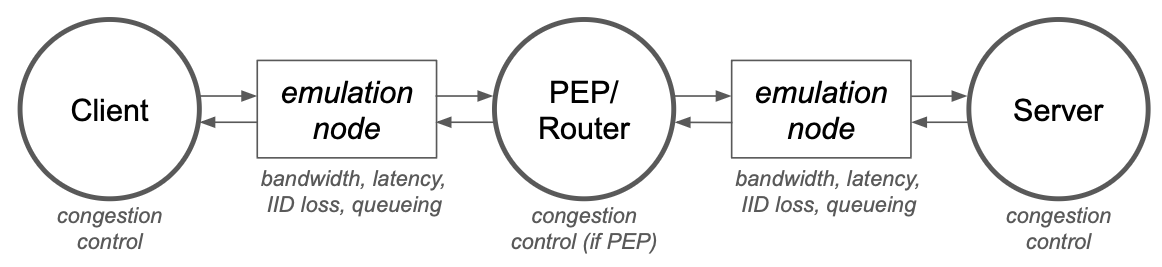
\includegraphics[width=\linewidth]{splitting-paper/figures/mininet-topology.png}
    \caption{Two-segment network topology in \texttt{mininet}. The
     middle node splits the path into two segments with different properties.}
    \label{fig:mininet}
\end{figure}

\begin{table}[t!]
  \centering
\footnotesize
\begin{tabular}{ l l l l l }
  \toprule
    \textbf{CCA} & \textbf{Implementation}\\
    \midrule
    BBRv3 & Linux TCP v6.4.0+ \texttt{google-bbr/v3} fork\\
    BBRv2 & Linux TCP v6.4.0+ \texttt{google-bbr/v2alpha} fork\\
    BBRv1 & Linux TCP v5.15.0-122-generic \\
    CUBIC & Linux TCP v5.15.0-122-generic \\
    % TCP & BBRv1 & Ubuntu 22.04.2 with Linux kernel 6.1, 6.8; Ubuntu 18.04.1 with Linux kernel\\
    % & & 4.15, 4.16, 4.17, 4.18, 5.0, 5.4, 5.19; Ubuntu 18.04.1 with Linux kernel v4.9,\\
    % & & 4.10, 4.11, 4.12, 4.14 (Docker Ubuntu 16.04 for build)\\
    BBRv3 & Google \texttt{quiche} v131.0.6728.1 \\
    BBRv1 & Google \texttt{quiche} v131.0.6728.1 \\
    CUBIC & Google \texttt{quiche} v131.0.6728.1 \\
    BBRv2 & Cloudflare \texttt{quiche} v0.14 \\
    BBRv1 & Cloudflare \texttt{quiche} v0.14 \\
    CUBIC & Cloudflare \texttt{quiche} v0.14 \\
    BBRv2 & IETF \texttt{picoquic} \texttt{29c7c53} \\
    BBRv1 & IETF \texttt{picoquic} \texttt{29c7c53} \\
    CUBIC & IETF \texttt{picoquic} \texttt{29c7c53} \\
\bottomrule
\end{tabular}
  \caption{\small \label{tab:cca-implementations} The congestion control schemes and
   transport protocol implementations we evaluate in the measurement study.}
  \vspace{-0.4cm}
\end{table}


We want to evaluate different congestion control schemes in a variety of network
settings. To do this, we run emulation experiments in \texttt{mininet} with
simple HTTPS clients and servers to measure the throughputs of long-lived data
transfers. In this section,
we describe our emulated network configurations, HTTPS endpoints and
PEP, and other specifications.

\paragraph{Network configuration.}

We used two linear network topologies: a one-segment topology for caching
end-to-end measurements and a two-segment topology for evaluation with a
connection-splitting PEP (\Cref{fig:mininet}). Both have
a client and server node at each end. The two-segment topology additionally has
a router node in between. Each path segment has a bridging node to emulate network
properties on the link.

We parameterize each path segment in three dimensions: delay, bandwidth, and a
random loss rate. We configure the network properties on the bridging nodes'
egress interfaces, using \texttt{tc-netem} to set delay and random loss,
and \texttt{tc-htb} to set bandwidth. Additionally, we use \texttt{tc-qdisc} to
configure the queues to use RED\footnote{We apply RED and not droptail because it gives more
continuous feedback about loss for congestion control, and is commonly used in
core routers. We also do not need the multi-flow and low-delay properties of
other queue disciplines. We use RED in \texttt{adaptive harddrop} mode with a
maximum queuing delay of $\approx1$ BDP. Exact parameters are available in the code.},
which is the source of congestive loss.
Each link is symmetric in
the uplink and downlink directions. For some versions of BBR, we set an \texttt
{fq} qdisc on the host nodes' egress interfaces for pacing.

\paragraph{Host configuration.}

We create simple HTTPS wrappers around each transport protocol implementation to
evaluate the congestion control schemes in \Cref{tab:cca-implementations}. The TCP
endpoints use the Python \texttt{http} module. For the QUIC implementations, we
modify comparable client/server applications from each repository.
%to transfer some number of bytes from server to client.
With the exception of enabling TCP pacing where required by BBR, we use
``default values'' for tunable parameters, considering these to be part of each
implementation.

In TCP, we set the CCA by using a specific Linux kernel
version and loading the congestion control module. We use the default
kernel's implementations of CUBIC and BBRv1, and Google's kernel fork for
BBRv2 and BBRv3 (\Cref{tab:cca-implementations}).

In QUIC, we simply select the CCA as a command-line
argument to the user space implementation. We evaluate Google \texttt
{quiche}~\cite{google-quiche}, Cloudflare \texttt{quiche}~\cite
{quiche}, and \texttt{picoquic}~\cite{picoquic}. Google and Cloudflare \texttt
{quiche} are their production implementations of the same name,
and \texttt{picoquic} is a minimalist implementation based on the IETF spec.
All three include CUBIC and BBRv1 implementations, as well as some form of
BBRv2 or BBRv3, which is still undergoing standardization.

For the transparent, connection-splitting TCP PEP, we use PEPsal~\cite
{caini2006pepsal}. PEPsal intercepts the SYN packet during the three-way
handshake and forms separate TCP connections with each endpoint,
copying data between the two sockets. Note that
discussions of split QUIC are based only on the split throughput heuristic
and do not use an actual splitter.

\paragraph{Experiment specification.}
In each experiment, the HTTPS client requests a specific number of bytes to be
transferred from the server in the HTTPS payload. This number corresponds to the
amount of data that can be transmitted through the bottleneck link over a
$10$-second period. We have found this to be sufficiently large to reflect
sustained throughput.

In practice, we report the "single-stream goodput" calculated as the number of
application-layer bytes received (excluding HTTPS headers) divided by request
completion time (from when the client sends a request to when it receives a
complete response). Due to header overhead and request latency, this metric
will never equal the link rate.

\paragraph{Machine specification.} All experiments use CloudLab~\cite
 {duplyakin2019design} x86\_64 rs630 nodes in the Massachusetts cluster running
 Ubuntu 22.04.2. The nodes use the default Linux kernel v5.15.0-122-generic,
 except for TCP BBRv2 and BBRv3.%, in which they use the Google fork of v6.4.0+.

\section{Measurement Study Results}
\label{sec:splitting:results}

\begin{figure*}[t!]
    \centering
    \begin{subfigure}[b]{0.22\linewidth}
        \centering
        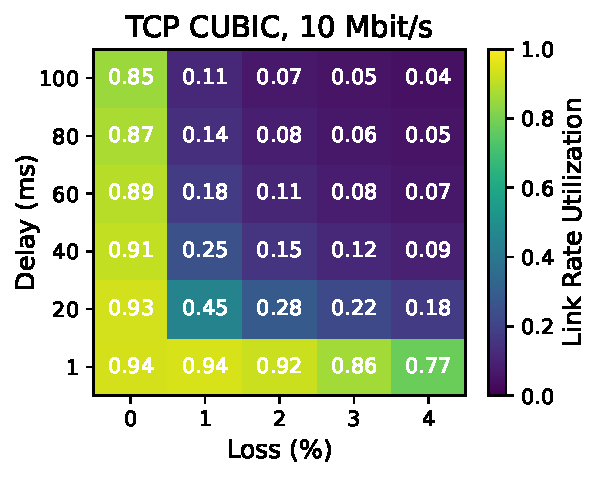
\includegraphics[width=\linewidth,trim={0 0 2cm 0.7cm},clip]
         {splitting-paper/figures/heatmaps/heatmap_tcp_cubic_10mbps.pdf}
        \captionsetup{skip=4pt}
        \caption{TCP CUBIC.}
        \label{fig:2d-heatmap:cubic-10}
    \end{subfigure}
    \begin{subfigure}[b]{0.22\linewidth}
        \centering
        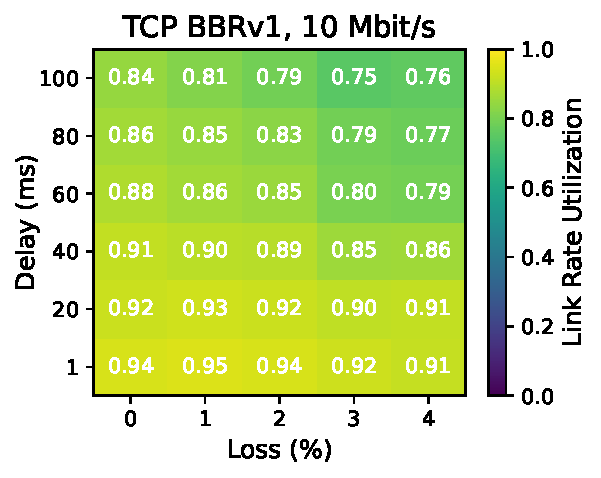
\includegraphics[width=\linewidth,trim={0 0 2cm 0.7cm},clip]
         {splitting-paper/figures/heatmaps/heatmap_tcp_bbr1_10mbps.pdf}
        \captionsetup{skip=4pt}
        \caption{TCP BBRv1.}
        \label{fig:2d-heatmap:bbr1-10}
    \end{subfigure}
    \begin{subfigure}[b]{0.22\linewidth}
        \centering
        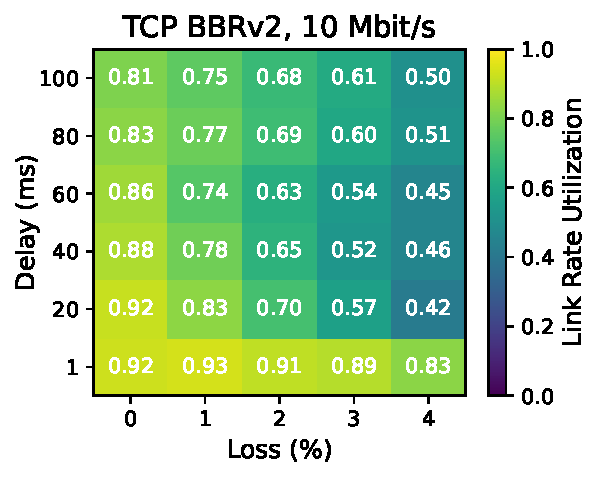
\includegraphics[width=\linewidth,trim={0 0 2cm 0.7cm},clip]
         {splitting-paper/figures/heatmaps/heatmap_tcp_bbr2_10mbps.pdf}
        \captionsetup{skip=4pt}
        \caption{TCP BBRv2.}
        \label{fig:2d-heatmap:bbr2-10}
    \end{subfigure}
    \begin{subfigure}[b]{0.22\linewidth}
        \centering
        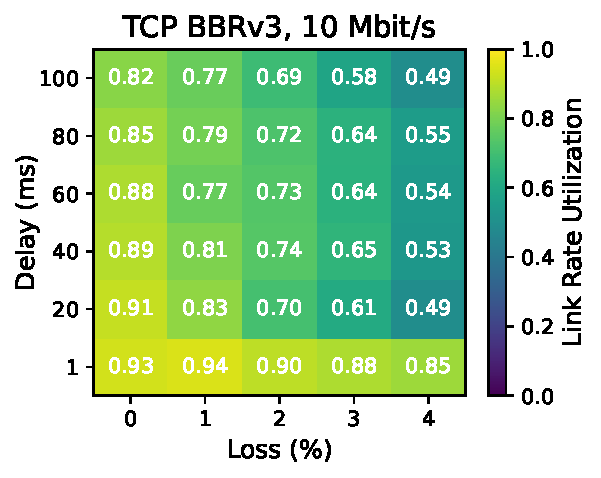
\includegraphics[width=\linewidth,trim={0 0 2cm 0.7cm},clip]
         {splitting-paper/figures/heatmaps/heatmap_tcp_bbr3_10mbps.pdf}
        \captionsetup{skip=4pt}
        \caption{TCP BBRv3.}
        \label{fig:2d-heatmap:bbr3-10}
    \end{subfigure}
    \begin{subfigure}[b]{1cm}
        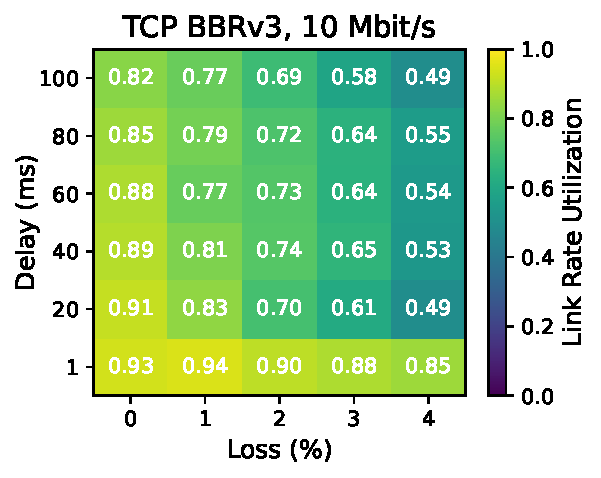
\includegraphics[width=1cm,trim={8cm 0 0 0},clip]
         {splitting-paper/figures/heatmaps/heatmap_tcp_bbr3_10mbps.pdf}
    \end{subfigure}
    \caption{The link rate utilization calculated as the ratio of achieved
     goodput to link rate for various TCP CCAs in an emulated network path, at
     various loss rates and one-way delays, at 10 Mbit/s. CUBIC is the
     most sensitive to loss and delay, while BBRv1 is the most aggressive and
     achieves the highest utilizations; BBRv2 and BBRv3 are more sensitive to
     loss than BBRv1 and utilization starts to suffer (left to right). CCAs
     tend to achieve lower utilizations, though higher absolute goodputs, as
     the link rate increases (\Cref{sec:appendix}). Median of $n=20$ trials.}
    \label{fig:2d-heatmap}
\end{figure*}


In our emulation measurement study, we aim to answer three questions to gain a
more comprehensive understanding of the relevance of connection-splitting with
modern networks:

\begin{enumerate}[noitemsep]
    \item Has the model-based BBR algorithm made the throughput enhancements of
     connection-splitting obsolete?
    \item Are there classes of network settings where BBR benefits significantly
     from splitting but CUBIC does not?
    \item How does CCA implementation impact end-to-end behavior, and therefore split
     behavior?
\end{enumerate}

\noindent To recap our measurement methodology, we have a method for
 measuring the throughput of TCP connections in emulation both with and without a
 transparent PEP. We also have the ability to estimate throughput both with and
 without a generic connection splitter, for both TCP and QUIC, based on
 knowledge of the network model of each path segment, and the measured end-to-end
 throughput on each segment.

For our analysis, we cache measurements for the end-to-end network parameters
in \Cref{tab:parameters} and the congestion control schemes in \Cref
{tab:cca-implementations}. We also run experiments in the two-segment network topology
to validate some of these predictions. Raw data for the end-to-end
behavior of each CCA implementation are available in \Cref{sec:appendix}.
Our emulation benchmarks are also publicly available on GitHub: \url{https://github.com/StanfordSNR/connection-splitting}.

\subsection{Finding 1: TCP BBR Over Time}
\label{sec:splitting:results:finding1}

\paragraph{Finding: Splitting has become significantly more beneficial to TCP
 BBR since it was initially released in 2016.}

Has the model-based BBR algorithm made the throughput enhancements of
connection-splitting obsolete? We find this line of thought has some truth
with the initial release of TCP BBRv1 in 2016. But as the BBR algorithm has
evolved into BBRv2 in 2019 and now BBRv3 in 2023, it has also evolved to behave
more conventionally in the sense that it benefits from being split---just like
more traditional, loss-based congestion control schemes such as CUBIC.

\Cref{fig:bbr-over-time} shows three different network settings in which BBRv2
and BBRv3 show significant throughput gains from connection-splitting.
 When BBRv1 was released, its throughput both with and
 without the connection-splitter were roughly the same, and nearly achieved the
 bottleneck link rate. With BBRv2 and BBRv3, the end-to-end throughput
 drastically deteriorated, behaving more like CUBIC than BBRv1. However, the
 split throughput remained relatively high, suggesting that BBRv3 today would
 still benefit from connection-splitting.

\paragraph{Analysis.}
To explore why CUBIC and BBRv3 benefit from splitting but BBRv1 does not, we
analyze end-to-end throughputs of each CCA and apply the split throughput
heuristic (\Cref{fig:heuristic}). As described in \Cref{sec:splitting:heuristic},
this methodology allows us to study split settings by measuring the much smaller
parameter space of end-to-end connections. We find that connection-splitting is
likely to improve throughput on lossy paths for CUBIC, BBRv2, and BBRv3
connections, but not for BBRv1.

\Cref{fig:2d-heatmap} visualizes our cached end-to-end measurements as link rate
 utilization heatmaps of loss vs. delay.
 Here is an example for how to interpret these graphs using \Cref
 {fig:2d-heatmap:bbr3-10}. The top-left cell represents a 100 ms 0\% segment
 with 0.82 utilization of the 10 Mbit/s link rate, and the bottom-right cell
 represents a 1 ms 4\% segment with 0.85 utilization of the 10 Mbit/s link
 rate. The predicted split utilization of a network path composed of these two
 segments is just 0.82, the minimum. The two cells compose to the top-right
 cell, which represents a 100 ms 4\% 10 Mbit/s segment with an end-to-end
 utilization of 0.49. Since $0.82>0.49$, we say that splitting has improved the
 throughput of this network path.

BBRv1 achieves high link rate utilization in all settings (\Cref
{fig:2d-heatmap:bbr1-10}), showing it has little to gain from splitting.
In fact, previous studies have shown that BBRv1 achieves $\approx\!85\%$
link utilization regardless of loss (same as our findings) before it reaches
a cliff point at around 20\% loss~\cite{cao2019use,cardwell2017bbr}.
This may be why it appears that splitting in lossy settings is now obsolete with BBR.
However, one should note that BBRv1's high throughput has long been attributed
to its aggressiveness and unfairness to legacy algorithms~\cite
{ware2019modeling,cao2019use}, which is what led to the changes in BBRv2 and
BBRv3.

While BBRv2 is a large departure from BBRv1, BBRv3 has been described as BBRv2
with bugfixes and performance tuning~\cite{cardwell2024bbrv3-ietf119}, which
supports why the two are so similar. We focus on BBRv3 since Google hopes to
now deprecate BBRv2~\cite{cardwell2024bbrv3-ietf119}.

BBRv3 is more sensitive to loss than its previous versions (\Cref
{fig:2d-heatmap:bbr3-10}), and more similar to CUBIC (\Cref
{fig:2d-heatmap:cubic-10}) in that there exist scenarios where end-to-end
throughput suffers.
These reflect existing findings of lower utilization in BBRv2 and BBRv3~\cite
{datta2023replication,song2021understanding,zeynali2024promises}.
Based on the heuristic, it is clear that in some lossy networks
such as the ones empirically evaluated in \Cref{fig:bbr-over-time},
connection-splitting
can significantly increase the throughput of BBRv3 connections.
It is possible that the BBR algorithm continues to evolve in this direction
given that BBR's unfairness remains contentious today~\cite
{datta2023replication,zeynali2024promises}.

\paragraph{Summary.}

While BBR may not have benefited from splitting with the release of ``v1'' in 2016, BBRv2 and
now BBRv3 have evolved to behave more conventionally---similar to traditional,
loss-based CCAs such as CUBIC---in the sense that they \textit{do}. Even
so-called ``model-based'' congestion control algorithms seem to now react to
loss as a congestion signal, as the BBR algorithm continues to evolve.

\subsection{Finding 2: TCP BBRv3 vs. TCP CUBIC}
\label{sec:splitting:results:finding2}

\paragraph{Finding: There exist classes of network paths where TCP BBRv3 would
 significantly benefit from splitting but TCP CUBIC would not.}

Are there new classes of network settings where BBR benefits significantly from
splitting but CUBIC does not? We want to understand the network settings in
which a congestion control scheme is not able to achieve practical bottleneck
link rate utilizations end-to-end, but is with a connection-splitter.

We find that while splitting benefits BBRv3 in all the same scenarios as CUBIC,
it also has the potential to benefit BBRv3 in many \textit{new} scenarios.
In addition to edge deployments with a lossy last-mile, BBRv3
also benefits from splitting in scenarios where there is loss on both path
segments, and when the connection-splitter is located farther from the edge.
We partition these scenarios into three classes of network settings:

\begin{enumerate}[label=\Roman*.,noitemsep]
\item Paths with asymmetric delay and a lossy last-mile,
\item Lossy paths with asymmetric delay,
\item Lossy paths with more symmetric delay.
\end{enumerate}

\noindent \Cref
 {fig:bbr-over-time:class1,fig:bbr-over-time:class2,fig:bbr-over-time:class3}
represent network settings in each class, respectively.
``Asymmetric'' refers to the delays on the two path segments.
These emulations empirically demonstrate that CUBIC only benefits in the first
class, while BBRv3 benefits in all three.
BBRv1 does not need splitting in any context.

\paragraph{Analysis.}
To identify which network paths benefit from connection-splitting and where
along the paths PEPs should be deployed, we apply the
heuristic (\Cref{fig:heuristic}).
For each CCA, we conduct an exhaustive search of the $15 \cdot 21 \cdot 25 =
7875$ combinations of settings within our parameter space (\Cref
{tab:parameters}), and efficiently predict the split and end-to-end throughputs.

We filter on the predicted throughputs for network settings where splitting improves end-to-end throughput by
at least $3\times$, and where the split connection utilizes at least half the
bottleneck link rate (\Cref{tab:network-path-analysis}). BBRv1 does not meet
these criteria is any scenarios, and the theoretical connection-splitter is
unable to improve the throughput of BBRv1 by even $50\%$. CUBIC and BBRv3 meet
these criteria in 942 and 188 scenarios, respectively. CUBIC benefits from
splitting in more scenarios because its end-to-end utilization is more
frequently low, so it more frequently has a large split improvement.

\begin{table}[t!]
  \centering
\begin{tabular}{ r l l l }
  \toprule
    \textbf{Filter} & \textbf{BBRv1} & \textbf{CUBIC} & \textbf{BBRv3} \\
    \midrule
    Initial & 7875 & 7875 & 7875 \\
    Split imprvmnt. $>3\times$ & 0 & 2231 & 234 \\
    Split utilization $>0.5$ & 0 & 942 & 188 \\
    \midrule
    Asymmetric, last-mile & 0 & 942 & 38 \\
    Asymmetric, lossy & 0 & 0 & 72 \\
    Symmetric, lossy & 0 & 0 & 78 \\
    \bottomrule
\end{tabular}
  \caption{\label{tab:network-path-analysis} An exhaustive search of network
   paths and their PEP locations that benefit from splitting for each CCA, and
   the number of filtered settings that belong to each class.}
  \vspace{-0.4cm}
\end{table}


Since the distribution of network paths in our parameter space does not reflect
any meaningful real world distribution, we are more interested in the \textit
{classes} of network settings that benefit from splitting. We realized
that \textit{all} of the relevant network settings for CUBIC can be clustered
into Class I, as network paths where one path segment has $1$ ms delay and
non-zero loss, and the other has $>1$ ms delay and $0\%$ loss. However, Class
I only accounts for $21\%$ of the relevant network settings for BBRv3. We
identify Class II, which is the same as I, except both path segments have
non-zero loss. Class III is the same as II, except both path segments have
$>1$ ms delay. We used the results to select three representative network
settings to empirically evaluate in \Cref{fig:bbr-over-time}.

Intuitively, we can understand why BBRv3 benefits more from splitting in lossy
scenarios than CUBIC based on how it reacts to loss and delay (\Cref
{fig:2d-heatmap:bbr3-10}). BBRv3's sensitivity to loss
and delay is more gradual than abrupt, so it is more likely to benefit when
splitting a lossy, high-delay network path in any way. In comparison, CUBIC's
throughput falls off a cliff for many of these segmentations.

\paragraph{Discussion.}
Do these results reflect where PEP deployments have been useful in the real
world? Connection-splitters have traditionally been found in satellite,
cellular, and Wi-Fi networks with a wireless link or rate policer~\cite
{edeline2019bottomup,honda2011still}. This resembles Class I, where the
network path consists of a lossy last-mile, and a reliable Internet path
segment. It makes sense then for PEPs to be traditionally located at the edge
to address the issues of loss-based schemes~\cite
{cloudsplitting2010,rfc3135,farkas2012splittcp}. We expect these PEPs to
similarly benefit BBRv3 in the same locations.

In Classes I and II, asymmetric delay can be severe in low-resource networks
in addition to wireless last-mile links;
Consider, for example, regions with no IXPs in which a significant proportion
of Internet traffic travels internationally.

For Classes II and III, satellite (and also wireless ad-hoc)
networks are known for
having lossy ``middle-miles''~\cite{kuhn2021quic-over-sat,border2020evaluating,pirovano2013new,cloudsplitting2010}.
This can be due to bad weather, fast-moving satellites, and
long-distance radio waves, etc.
Since CUBIC does not trivially benefit from splitting in these scenarios, the
traditional solution has been to split the connection at multiple points and to
use an FEC-based or other proprietary protocol in the satellite backhaul~\cite
{cloudsplitting2010,border2020evaluating,rfc3135}.
Our results suggest such an invasive solution may not be necessary for BBRv3.

How could this inform the deployment of connection-splitting PEPs?
With the caveat that futher exploration is required to understand how the
heuristic extrapolates to the real world, one idea is to
determine where to deploy PEPs along an existing network path for maximum
benefit especially as congestion-control schemes evolve.
Another idea is given the location of a PEP, determine which connections going
through the PEP would most benefit based on knowledge of each connection's
network path.
We leave network operators to decide how best to model their networks and apply
the heuristic to evaluate potential PEP deployments.

\paragraph{Summary.}
While TCP CUBIC only benefits from connection-splitting when the PEP is located
at the lossy last-mile, TCP BBRv3 can also benefit when there is loss on both
sides of the PEP and when there are longer propagation delays. This suggests
that TCP connections using BBRv3 should benefit from splitters at the same
locations as for CUBIC, and also that traditional methods used to
address loss in the middle-mile could use simple connection-splitting instead.
We believe this method of analyzing useful network paths and PEP placements for
connection-splitting can be extended to model new types of networks, especially
in space.

\subsection{Finding 3: QUIC Congestion Control}
\label{sec:splitting:results:finding3}

\paragraph{Finding: QUIC implementations of the same congestion control schemes
 vary significantly, and further differ from Linux's TCP implementations.}

\begin{figure*}[t!]
    \centering
    \begin{subfigure}[b]{0.22\linewidth}
        \centering
        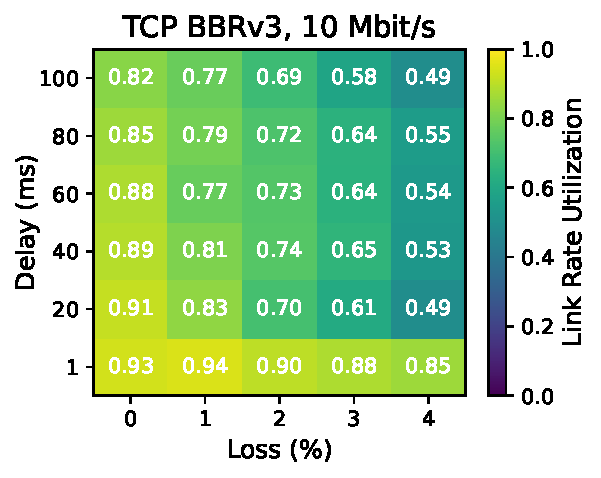
\includegraphics[width=\linewidth,trim={0 0 2cm 0.7cm},clip]
        {splitting-paper/figures/heatmaps/heatmap_tcp_bbr3_10mbps.pdf}
        \captionsetup{skip=4pt}
        \caption{TCP, BBRv3}
        \label{fig:quic:tcp-bbr3}
    \end{subfigure}
    \begin{subfigure}[b]{0.22\linewidth}
        \centering
        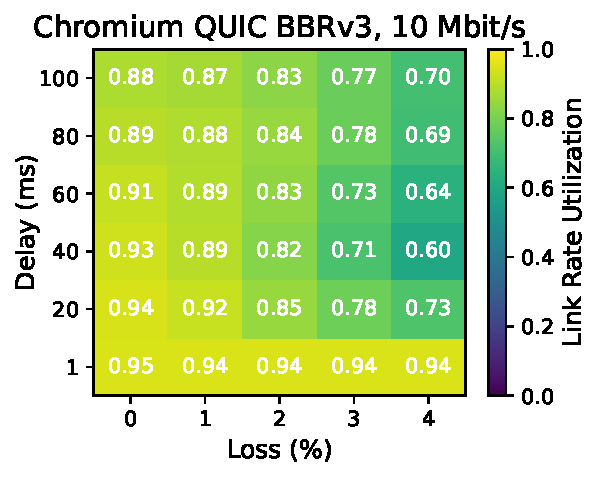
\includegraphics[width=\linewidth,trim={0 0 2cm 0.7cm},clip]
        {splitting-paper/figures/heatmaps/heatmap_quic_bbr3_10mbps.pdf}
        \captionsetup{skip=4pt}
        \caption{Google \texttt{quiche}, BBRv3}
        \label{fig:quic:google-bbr3}
    \end{subfigure}
    \begin{subfigure}[b]{0.22\linewidth}
        \centering
        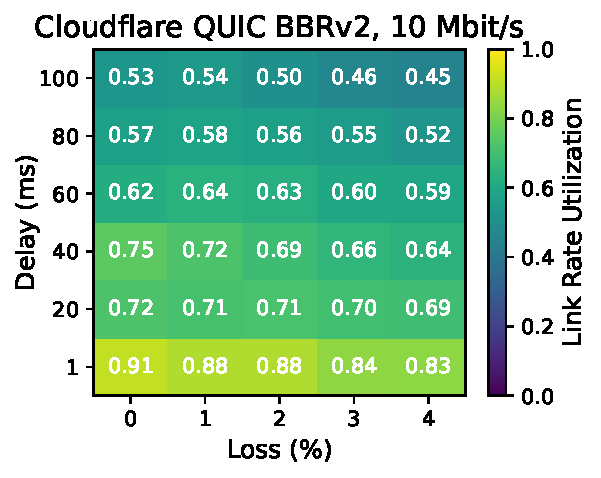
\includegraphics[width=\linewidth,trim={0 0 2cm 0.7cm},clip]
        {splitting-paper/figures/heatmaps/heatmap_quiche_bbr2_10mbps.pdf}
        \captionsetup{skip=4pt}
        \caption{Cloudflare \texttt{quiche}, BBRv2}
        \label{fig:quic:cloudflare-bbr2}
    \end{subfigure}
    \begin{subfigure}[b]{0.22\linewidth}
        \centering
        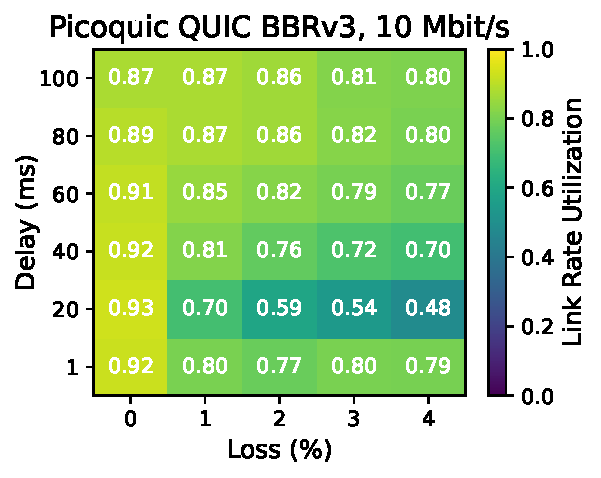
\includegraphics[width=\linewidth,trim={0 0 2cm 0.7cm},clip]
        {splitting-paper/figures/heatmaps/heatmap_picoquic_bbr3_10mbps.pdf}
        \captionsetup{skip=4pt}
        \caption{\texttt{picoquic}, BBRv3}
        \label{fig:quic:picoquic-bbr3}
    \end{subfigure}
    \begin{subfigure}[b]{1cm}
        \includegraphics[width=1cm,trim={8cm 0 0 0},clip]
        {splitting-paper/figures/heatmaps/heatmap_tcp_bbr3_10mbps.pdf}
        \vspace*{0.2cm}
    \end{subfigure}
    
    \begin{subfigure}[b]{0.22\linewidth}
        \centering
        \includegraphics[width=\linewidth,trim={0 0 2cm 0.7cm},clip]
        {splitting-paper/figures/heatmaps/heatmap_tcp_bbr1_10mbps.pdf}
        \captionsetup{skip=4pt}
        \caption{TCP, BBRv1}
        \label{fig:quic:tcp-bbr1}
    \end{subfigure}
    \begin{subfigure}[b]{0.22\linewidth}
        \centering
        \includegraphics[width=\linewidth,trim={0 0 2cm 0.7cm},clip]
        {splitting-paper/figures/heatmaps/heatmap_quic_bbr1_10mbps.pdf}
        \captionsetup{skip=4pt}
        \caption{Google \texttt{quiche}, BBRv1}
        \label{fig:quic:google-bbr1}
    \end{subfigure}
    \begin{subfigure}[b]{0.22\linewidth}
        \centering
        \includegraphics[width=\linewidth,trim={0 0 2cm 0.7cm},clip]
        {splitting-paper/figures/heatmaps/heatmap_quiche_bbr1_10mbps.pdf}
        \captionsetup{skip=4pt}
        \caption{Cloudflare \texttt{quiche}, BBRv1}
        \label{fig:quic:cloudflare-bbr1}
    \end{subfigure}
    \begin{subfigure}[b]{0.22\linewidth}
        \centering
        \includegraphics[width=\linewidth,trim={0 0 2cm 0.7cm},clip]
        {splitting-paper/figures/heatmaps/heatmap_picoquic_bbr1_10mbps.pdf}
        \captionsetup{skip=4pt}
        \caption{\texttt{picoquic}, BBRv1}
        \label{fig:quic:picoquic-bbr1}
    \end{subfigure}
    \begin{subfigure}[b]{1cm}
        \includegraphics[width=1cm,trim={8cm 0 0 0},clip]
        {splitting-paper/figures/heatmaps/heatmap_tcp_bbr1_10mbps.pdf}
        \vspace*{0.2cm}
    \end{subfigure}

    \begin{subfigure}[b]{0.22\linewidth}
        \centering
        \includegraphics[width=\linewidth,trim={0 0 2cm 0.7cm},clip]
        {splitting-paper/figures/heatmaps/heatmap_tcp_cubic_10mbps.pdf}
        \captionsetup{skip=4pt}
        \caption{TCP, CUBIC}
        \label{fig:quic:tcp-cubic}
    \end{subfigure}
    \begin{subfigure}[b]{0.22\linewidth}
        \centering
        \includegraphics[width=\linewidth,trim={0 0 2cm 0.7cm},clip]
        {splitting-paper/figures/heatmaps/heatmap_quic_cubic_10mbps.pdf}
        \captionsetup{skip=4pt}
        \caption{Google \texttt{quiche}, CUBIC}
        \label{fig:quic:google-cubic}
    \end{subfigure}
    \begin{subfigure}[b]{0.22\linewidth}
        \centering
        \includegraphics[width=\linewidth,trim={0 0 2cm 0.7cm},clip]
        {splitting-paper/figures/heatmaps/heatmap_quiche_cubic_10mbps.pdf}
        \captionsetup{skip=4pt}
        \caption{Cloudflare \texttt{quiche}, CUBIC}
        \label{fig:quic:cloudflare-cubic}
    \end{subfigure}
    \begin{subfigure}[b]{0.22\linewidth}
        \centering
        \includegraphics[width=\linewidth,trim={0 0 2cm 0.7cm},clip]
        {splitting-paper/figures/heatmaps/heatmap_picoquic_cubic_10mbps.pdf}
        \captionsetup{skip=4pt}
        \caption{\texttt{picoquic}, CUBIC}
        \label{fig:quic:picoquic-cubic}
    \end{subfigure}
    \begin{subfigure}[b]{1cm}
        \includegraphics[width=1cm,trim={8cm 0 0 0},clip]
        {splitting-paper/figures/heatmaps/heatmap_tcp_cubic_10mbps.pdf}
        \vspace*{0.2cm}
    \end{subfigure}

    \caption{Heatmaps for three QUIC implementations of BBRv3 (or BBRv2), BBRv1,
     and CUBIC showing link rate utilization calculated as the ratio of
     achieved goodput to link rate, compared to Linux TCP. The heatmaps are
     shown at various loss rates and one-way delays with a fixed link rate of
     10 Mbit/s. User-space QUIC is not CPU-limited, achieving high utilizations
     at 1 ms delay and 0\% loss. The QUIC implementations are Google \texttt
     {quiche}, Cloudflare \texttt{quiche}, and a minimalist implementation
     based on the IETF spec called \texttt{picoquic}. Median of $n=20$
     trials.}
    \label{fig:quic}
    \vspace{-0.3cm}
\end{figure*}


How does CCA implementation impact end-to-end behavior, and therefore split
behavior? Might claims about ``split throughput'' depend not just on the CCA,
but also the \textit{implementation} and/or the transport protocol
on top of it?

For our initial study, we compared end-to-end throughput for four open-source
implementations each of CUBIC, BBRv1, and BBRv2/3; one using TCP and three
using QUIC. We find that the end-to-end behavior of each CCA varies by
implementation in both baseline throughput and sensitivity to loss and delay.
To evaluate the split behavior of QUIC, instead of creating a custom and
explicit connection-splitting PEP for each QUIC implementation, we apply the
split throughput heuristic and argue that these implementations
will likewise respond differently to connection-splitting PEPs.

\Cref{fig:quic} visualizes the end-to-end behavior of these schemes.
We highlight that the Cloudflare and \texttt
 {picoquic} CUBIC implementations are less sensitive to loss than Google or
 TCP; the former may benefit from splitting in more classes of network settings
 than the latter. Additionally, their BBR implementations exhibit non-uniform
 behavior, suggesting a non-uniform response to
 connection-splitting. These variations indicate that the benefits of
 in-network assistance should be considered along with not just the CCA but its
 specific implementations.

\paragraph{Analysis.}

The Google QUIC (\Cref{fig:quic:google-bbr1,fig:quic:google-bbr3,fig:quic:google-cubic})
and TCP (\Cref{fig:quic:tcp-bbr1,fig:quic:tcp-bbr3,fig:quic:tcp-cubic})
implementations are most similar to each other for each CCA.
This is reasonable if we take the community-based CUBIC implementation in
Linux to be the standard, and considering that Google contributed to the Linux
BBR implementations. In general, Google QUIC achieves slightly higher
utilization than Linux TCP.

The Cloudflare QUIC BBR implementations (\Cref{fig:quic:cloudflare-bbr1,fig:quic:cloudflare-bbr2})
exhibit profoundly different behavior from Linux TCP in baseline performance.
Note that Cloudflare uses BBRv1 for TCP but their use of BBR in QUIC
is experimental. Anecdotally, a
Cloudflare employee has expressed difficulty making
their BBR implementation performant, having to reverse engineer
the Linux kernel~\cite{cardwell2024bbrv3-ietf119-qna}. Given the wide adoption
of BBRv1 for TCP at many CDNs~\cite{ware2024ccanalyzer}, we expect it to
be desirable yet challenging for these same companies to correctly incorporate
BBRv3 into their QUIC stacks in the coming years.
% Maybe cite narayan2018restructuring

The \texttt{picoquic} BBR implementations (\Cref{fig:quic:picoquic-bbr1,fig:quic:picoquic-bbr3})
are more similar to Linux TCP, although its BBRv3 implementation seems to have
a contradicting reaction to delay.
We note that \texttt{picoquic} is intended for experimental use in the
IETF~\cite{picoquic}. It is important then to understand its congestion control
behavior if it is to be used to evaluate
IETF proposals. We believe its differences from Linux TCP warrant further
exploration, but perhaps also that the ongoing standardization efforts of BBR
in the IETF~\cite{cardwell2024bbr-ietf-draft} indicate
that there is no monolith yet of ``the BBR algorithm.''

The Cloudflare QUIC and \texttt{picoquic} implementations of CUBIC
(\Cref{fig:quic:cloudflare-cubic,fig:quic:picoquic-cubic}) interestingly
both exhibit a more gradual degradation in response to loss and delay than Linux TCP
(\Cref{fig:quic:tcp-cubic}). We
find this harder to explain, given that TCP CUBIC has been around since 2006,
and perhaps can be attributed to transport protocol mechanisms in QUIC.
Nevertheless, this indicates that it is important to understand the
behavior of a CCA in the context of its entire
implementation.

\begin{figure}[t!]
    \centering
    \begin{subfigure}[b]{\linewidth}
        \centering
        \includegraphics[width=0.8\linewidth]
         {splitting-paper/figures/network_path_analysis/network_path_analysis_10_40_1_80_2_2.pdf}
        \captionsetup{skip=0pt}
        \caption{Some QUIC CUBIC implementations can benefit in new network
         classes where TCP CUBIC could not.}
        \label{fig:quic-predictions:cubic}
    \end{subfigure}
    \begin{subfigure}[b]{\linewidth}
        \centering
        \includegraphics[width=0.8\linewidth]
         {splitting-paper/figures/network_path_analysis/network_path_analysis_40_50_20_1_0_4.pdf}
        \captionsetup{skip=0pt}
        \caption{The various BBRv3 implementations have non-uniform end-to-end
         behavior and no clear resulting split behavior.}
        \label{fig:quic-predictions:bbr3}
    \end{subfigure}
    \caption{Predicted bottleneck link rate utilizations calculated from the
     predicted end-to-end and split throughputs of the TCP and QUIC
     implementations, on two different network path segments. End-to-end
     behavior of each CCA varies significantly by implementation.}
    \label{fig:quic-predictions}
\end{figure}


\Cref{fig:quic-predictions} applies the heuristic to show how split behavior
can vary for CCA implementations with different end-to-end behaviors.
Some QUIC CUBIC implementations
benefit in new network settings where TCP CUBIC does not, while the various
QUIC BBRv3 implementations exhibit non-uniform end-to-end behavior and thus no
clear trend in split behavior.

\paragraph{Discussion.}

Why do we believe we can extrapolate split behavior from the end-to-end behavior
of QUIC? Previous studies explore the effects of QUIC's transport protocol
mechanisms in such a case~\cite{kosek2022quicpep,thomas2019google}. They find
that the effects of zero-RTT connection establishment with regards to
long-lived throughput to be minimal, and stream multiplexing to be mutually
beneficial in both scenarios. Further studies can clarify the interactions
between CCAs and transport mechanisms.

How do we know that the difference in behavior is due to the congestion control
implementation and not other transport protocol mechanisms? Well, we
don't, and there is known to be significant variance in the features supported
by different QUIC implementations~\cite{marx2020same}.
However, we find it intuitive that congestion control would be a major factor in
the measured sustained goodput of a bulk file transfer.

The divergence in QUIC implementations is not so dissimilar from that of TCP at
a similar state of evolution~\cite{allman1999effective}, but there are still
some fundamental differences. With QUIC implementations in userspace, there is
a larger diversity of implementations that are easier to tune for a specific
application metric, as opposed to correctness or fairness from a
congestion-control point of view. These algorithms are also highly
parameterized, with no standard nor test suite, so it's not surprising that the
implementations differ.

If there is reason to believe
that QUIC is losing out on throughput by not connection-splitting, then there
will continue to be research on how to achieve the same benefits without
ossification~\cite{kosek2023secure,yuan2024sidekick,kramer2021masquepep,yuan2022sidecar}.
The heuristic helps us understand the theoretical achievable
throughput with a simple connection-splitter, or even by combining multiple
end-to-end congestion control schemes.
In addition to research, this could motivate privacy-minded proposals in the Internet
standards community to also view themselves as potential deployment opportunities
for private PEPs~\cite{kosek2021masque,sattler2022towards,rfc9297,rfc9298}.

Another application of analyzing CCA implementations is to analyze the Linux TCP
implementations of BBR \textit{within} a major version over time. We did
this analysis with BBRv1 on 13 Linux kernels between 2016 and 2024, but found
no significant variance. However, given the dynamic nature of BBR and the
Linux networking stack, it
is possible there will still be changes to the split behavior of TCP in the future.

\paragraph{Summary.}

We believe it is important to understand the end-to-end behavior of a congestion
control scheme in the context of its entire implementation.
Our results suggest that BBR is challenging to implement, and that even CUBIC
implementations can vary based on context. Whether the prevailing wisdom is
that a specific CCA or transport protocol has made in-network assistance
undesirable, these results suggest that it is valuable to consistently
re-evaluate these claims.

\section{Accuracy Analysis}
\label{sec:splitting:accuracy}

\begin{figure*}[t]
    \centering
    \begin{subfigure}[b]{0.325\linewidth}
        \centering
        \includegraphics[width=\linewidth,trim={0 0 25.8cm 0},clip]
         {splitting-paper/figures/accuracy/accuracy_e2e_without_loss.pdf}
        \includegraphics[width=\linewidth,trim={0 0 25.8cm 0},clip]
         {splitting-paper/figures/accuracy/accuracy_e2e_with_loss.pdf}
        \captionsetup{skip=4pt}
        \caption{End-to-end throughput accuracy.}
        \label{fig:accuracy:e2e}
    \end{subfigure}
    \begin{subfigure}[b]{0.645\linewidth}
        \centering
        \includegraphics[width=\linewidth,trim={0 0 13.4cm 0},clip]
         {splitting-paper/figures/accuracy/accuracy_split_without_loss.pdf}
        \includegraphics[width=\linewidth,trim={0 0 13.4cm 0},clip]
         {splitting-paper/figures/accuracy/accuracy_split_with_loss.pdf}
        \captionsetup{skip=4pt}
        \caption{Split throughput accuracy.}
        \label{fig:accuracy:split}
    \end{subfigure}

    \caption{Heatmaps of the measured and predicted BBRv3 throughputs for
     various splits of delay, bandwidth, and loss, both without (top) and with
     (bottom) loss.
     The \textit{end-to-end throughput} predictions (not pictured) are the same for all
     cells at 0.86 utilization without loss and 0.58 utilization with loss,
     because they represent the same network path, so end-to-end
     prediction errors are roughly uniform.
     The \textit{split throughput} predictions err slightly on the side of
     overestimation, but they accurately reflect trends in higher or lower throughputs for
     measurements on different splits of the same network path. Median of $n=40$ trials.}
    \label{fig:accuracy}
    \vspace{-0.3cm}
\end{figure*}


Our analysis of connection-splitting for TCP and its extensions to QUIC rely on
the accuracy of the split throughput heuristic. In this section, we are
primarily concerned with how accurate our predictions, which are based on
measurements from a one-segment topology, are for measurements from a
two-segment topology in emulation, without and with a connection-splitting TCP
PEP:
\begin{itemize}[noitemsep]
\item Does the \texttt{compose} function accurately represent the combined
 network path in the end-to-end throughput?
\item Does the split throughput heuristic accurately predict split throughput?
\end{itemize}

\noindent Most importantly, we find the heuristic to be able to usefully
 predict \textit{trends}.
 In terms of absolute predictions, we find the \texttt{pred\_e2e\_throughput()}
 and \texttt{pred\_split\_throughput()} functions to be correct within a
 reasonable tolerance, with a slight tendency to overestimate.

Orthogonally, we do not evaluate the accuracy to which emulation studies reflect
the real world with multi-flow settings and more complex network properties,
nor how the accuracy would extrapolate to QUIC connections with custom
connection splitters. It may be interesting to explore how to incorporate
such factors into the network model and heuristic.

\paragraph{Methodology.} Recall that for a given network path composed of two
 path segments, we can obtain both the predicted end-to-end and split
 throughputs, and the ground truth throughputs in an emulated network with and
 without a TCP PEP. Then for a network setting, we can compute the accuracy as
 the percent error in predicted vs. measured throughput.

We perform an empirical accuracy analysis of BBRv3 for two end-to-end network paths with
identical bandwidth and delay, both without (0\%) and with (4\%) loss. We test
various splits for the bandwidth, delay, and loss and analyze the accuracy
trends. In particular, we select delay splits such that the end-to-end delay is
80 ms, bandwidth splits such that the bottleneck bandwidth is 10 Mbit/s, and loss
splits such that the total loss is either 0\% or 4\%. We parameterize the network
path segments to use the cached measurements from \Cref
{tab:parameters}.

\paragraph{End-to-End Throughput Accuracy.}

Each of our splits composes to the same end-to-end network path, so we predict
the same end-to-end throughput for each. Our experimental
results in \Cref{fig:accuracy:e2e} show that the measured end-to-end
throughputs are also roughly uniform, especially without loss, indicating that
our method of composing network path segments in emulation represents the same
end-to-end network path.

\paragraph{Split Throughput Accuracy.}

The split throughput predictions accurately reflect trends in loss, delay, and
bandwidth (\Cref{fig:accuracy:split}). For example, split throughput is
generally higher when the high-bandwidth link is paired with high delay
(the yellow-est cells). It is also lower when the lossy link is paired with
high delay (columns 1 and 2) or low bandwidth (columns 3-5).

The split throughput predictions tend to slightly overestimate, but we think
the level of error is small enough to be helpful for informing real PEP
deployment. The maximum error is $\pm14\%$, and on average $\pm4\%$. This
dwarfs the measured gains in some situations, and rules out a large gain in
others.

One factor that may lead to overestimation of split throughput is the queue
behavior and the burstiness of the sender. With small queues and bursty
sending, we would expect the far path segment from the data sender to sometimes
be limited by the send buffer. This could subsequently affect how the far
connection probes for and utilizes available link rate capacity.

Another factor is the proximity of the bottleneck link to the sender. While
our heuristic does not account for this, the real split throughputs for
symmetric pairs of network paths (e.g., the left three and right three columns
in \Cref{fig:accuracy:split}), show that we slightly overestimate
when the low-bandwidth bottleneck link is far from the sender.
Based on our reasoning about queues, this would suggest that the far path
segment, already the bottleneck, is even further under-saturated.

Overall, we find our end-to-end and split throughput predictions to usefully
reflect relative trends and absolute throughput within a
reasonable tolerance. They are not intended to make claims about exact achievable
throughputs nor about the immediate utility of PEPs in the real world,
but simply to reason about how connection-splitting may impact
long-lived throughput in a simplified network model.

\chapter{Conclusion}
\label{sec:conclusion}

\section{Summary}
\label{sec:conclusion:summary}

\section{Future work}
\label{sec:conclusion:future}

% % \subsubsection{Real-world studies}
% Our emulations model non-congestive loss as random, independent loss,
% which may not accurately reflect the real world. While non-congestive loss
% does exists, its various behaviors are not well-characterized. This work
% would benefit from a measurement study on the patterns of non-congestive loss
% to better understand the scope of the problem and its impact.

% We base this work on the idea that proxies and link-layer approaches are
% deployed for a reason, and understanding the impact that encrypted transport
% protocols have in these real-world network paths would better motivate the need
% for protocol-agnostic proxies at all. This is also true on paths where
% reliable connectivity is not a solved problem. Also,
% in-network retransmissions intuitively reduce load in the network and it may be
% interesting to explore how these retransmissions benefit not just
% applications but the network itself.

% % \subsubsection{Deployment and standardization}
% The question for any research system is how can it be deployed and useful in
% the real world. The simplest deployment today could look like a simple in-line
% Packrat proxy between a Wi-Fi router and Internet modem. Public hotspots and
% dense urban apartments make good candidates for smaller-scale lossy path
% segments.
% The client integration could be a browser extension for QUIC or a simple
% modified media client.
% The Packrat protocol has the advantage that only one endpoint in addition to the
% proxy needs to speak the protocol.

% % \subsubsection{Set reconciliation in packet-scale settings}
% In this paper, we explored an alternative construction of the quACK that is
% optimized for computational efficiency at a small granularity. An extension to
% this is finding other applications of the quACK in the setting of network
% packet analysis. We may also be able to further improve the link overheads of
% the IBLT quACK at millisecond timescales using, e.g., interactive quACKing
% between the proxy and endpoint.

\section{Concluding Remarks}
\label{sec:conclusion:remarks}
...


\appendix
\chapter{Appendix}

\section{Intuitive analysis of PACUBIC}
\label{sec:appendix:pacubic}

\begin{figure*}[h]
\centering
\includegraphics[width=0.8\linewidth]{sidekick-paper/figures/cwnd/cwnd_legend.pdf}\\
\begin{subfigure}{0.32\linewidth}
	\includegraphics[width=\linewidth]{sidekick-paper/figures/cwnd/cwnd_split_loss0p.pdf}
	\caption{Split CUBIC, 0\% loss.}
	\label{fig:time-cwnd:split-loss0p}
\end{subfigure}
\begin{subfigure}{0.32\linewidth}
	\includegraphics[width=\linewidth]{sidekick-paper/figures/cwnd/cwnd_pacubic_loss0p.pdf}
	\caption{PACUBIC, 0\% loss.}
	\label{fig:time-cwnd:pacubic-loss0p}
\end{subfigure}
\begin{subfigure}{0.32\linewidth}
	\includegraphics[width=\linewidth]{sidekick-paper/figures/cwnd/cwnd_cubic_loss0p.pdf}
	\caption{CUBIC, 0\% loss.}
	\label{fig:time-cwnd:cubic-loss0p}
\end{subfigure}
\begin{subfigure}{0.32\linewidth}
	\includegraphics[width=\linewidth]{sidekick-paper/figures/cwnd/cwnd_split_loss1p.pdf}
	\caption{Split CUBIC, 1\% loss.}
	\label{fig:time-cwnd:split-loss1p}
\end{subfigure}
\begin{subfigure}{0.32\linewidth}
	\includegraphics[width=\linewidth]{sidekick-paper/figures/cwnd/cwnd_pacubic_loss1p.pdf}
	\caption{PACUBIC, 1\% loss.}
	\label{fig:time-cwnd:pacubic-loss1p}
\end{subfigure}
\begin{subfigure}{0.32\linewidth}
	\includegraphics[width=\linewidth]{sidekick-paper/figures/cwnd/cwnd_cubic_loss1p.pdf}
	\caption{CUBIC, 1\% loss.}
	\label{fig:time-cwnd:cubic-loss1p}
\end{subfigure}
\caption{Congestion window of a long-running upload in Scenario \#2
(\Cref{tab:experimental-scenarios}) with $0\%$ and $1\%$ loss on the near
path segmenet.
The cwnd is measured at the data sender,
except for split CUBIC whose split connection also has a cwnd at the proxy.
PACUBIC reacts to every congestion event while keeping the cwnd high.
CUBIC performs poorly when there is loss on the near path segment.
CUBIC and PACUBIC are implemented in QUIC, while split CUBIC is implemented
in TCP using a PEP.
}
\label{fig:time-cwnd}
\end{figure*}

Here, we dive deeper into the intuition behind the PACUBIC constants
(\Cref{sec:sidekick:protocol:sender-behavior}), including how they were derived and why the PACUBIC
algorithm achieves similar congestion behavior to the CUBIC algorithm in a split
connection---we call this behavior ``split CUBIC''.

Consider the same network topology as \Cref{fig:sc-protocols} in which a
data sender uploads a large file to a data receiver, with help from a Sidekick
proxy in the middle of the connection. The near path segment connects the sender
to the proxy, and the far path segment connects the proxy to the receiver.
The near segment is low-delay with varying random loss, and the far segment is
high-delay with no random loss. The far segment is the bottleneck link in terms
of bandwidth.
The actual link parameters are the same as in Scenario \#2 of
\Cref{tab:experimental-scenarios}.

We first discuss how split CUBIC would behave in this setting to conceptually
motivate PACUBIC.
Consider the congestion windows of each half of the
split connection, one taken at the data sender and one at the proxy
(\Cref{fig:time-cwnd:split-loss0p,fig:time-cwnd:split-loss1p}).
The far path segment experiences only congestive loss,
leading the window at the proxy to fluctuate around the segment's BDP
regardless of the loss on the near path segment.
The window at the data sender independently determines whether the packets
that reach the proxy will be able to fully utilize the window set at the far
path segment. The data sender is able to achieve this at low random loss rates, but
becomes the bottleneck as loss rates increase (\Cref{fig:loss-vs-tput}).

While split CUBIC has two windows, PACUBIC only has one
window representing the in-flight bytes of the end-to-end connection.
PACUBIC considers loss detected from both quACKs and end-to-end ACKs.
Conceptually, we want an algorithm that would enable PACUBIC's single
congestion window to match the sum of CUBIC's two congestion windows, or
the total number of in-flight bytes.
% That is the motivation behind adjusting the window proportionally to the
% number of in-flight bytes on each path segment, depending on where the loss occurred.

With no random loss on the near path segment, PACUBIC (\Cref{fig:time-cwnd:pacubic-loss0p})
behaves the same as normal CUBIC (\Cref{fig:time-cwnd:cubic-loss0p}).
The congestion window is entirely governed by end-to-end ACKs since
the far path segment is the bottleneck link. Note that while the sender may be
able to deduce that a loss occurred on the far path segment by combining info from
the quACK with the end-to-end ACK, PACUBIC conservatively treats the loss as
occurring anywhere on the path.

With some random loss on the near path segment, PACUBIC grows and reduces cwnd
based on where the last congestion event occurs (\Cref{fig:time-cwnd:pacubic-loss1p}).
Note that if the congestion window $cwnd$
represents the bytes in-flight in the end-to-end connection, then
$r \cdot cwnd$ represents the proportion of bytes in-flight on the near
path segment. At a high level, if the data sender discovers loss
on the near path segment via the quACK, it holds the $(1-r)\cdot cwnd$ portion of
the ``far window'' constant while applying the CUBIC algorithm to the remaining
$r \cdot w_{max}$ of the ``near window,'' representing the bottleneck link.

Mathematically, instead of reducing $w_{max}$, the window size just before the
last reduction, by $(1-\beta^*) \cdot w_{max}$, PACUBIC reduces it by only
$[1 - (1-r(1-\beta^*))] \cdot w_{max} = r(1-\beta^*) \cdot w_{max}$.
That is $r$ times the original reduction, a \emph{smaller} amount.
We use the RTT ratio $r$ (near path segment to end-to-end)
% indicating the RTT ratio of near path segment vs.~far path segment)
as a proxy for the ratio of the number of in-flight bytes.

Similarly, instead of using a cubic growth function with scaling factor $C^*$
and inflection point $K = K^* = \sqrt[3]{w_{max}(1-\beta^*)/C^*}$,
we use a larger scaling factor $C = C^*/r^3$
and thus a shorter inflection point
\[
K = \sqrt[3]{\frac{w_{max}(1-\beta)}{C}}
= \sqrt[3]{\frac{r\cdot w_{max}(1-\beta^*)}{C^* / r^3}}
= r^{4/3} \cdot K^*.
\]
The shorter inflection point leads the congestion window to \emph{grow more
quickly} since the sender also reacts to feedback about loss more quickly over
the low-delay link.
% Since
% similarly proportional to $w_{max}$, so with $C'$, we both reduce the inflection
% point $K$ and the growth rate $C$ of the function proportionally to the
% number of bytes in-flight on the near path segment.

At times, there can be loss detected both in quACKs and in end-to-end ACKs.
The end-to-end ACKs have a greater effect since they reduce the congestion
window by a larger proportion, until the remaining path segment with loss is the
bottleneck link. In this scenario with loss, the bottleneck link at equilibrium
is the near path segment.
At this point, the quACK primarily determines the congestion window updates.
If the far path segment were to become the bottleneck again, the data sender would
detect a congestion event via the end-to-end ACK.

PACUBIC has several limitations. Although it beats end-to-end CUBIC, it
still performs worse than split CUBIC, especially at
high loss rates (\Cref{fig:loss-vs-tput}). Also, it doesn't consider loss on the
far path segment any differently than original CUBIC, unlike split CUBIC
which treats the two split connections independently. PACUBIC
emulates the congestion control behavior and fairness of split CUBIC
fairly well as a heuristic, but would benefit from an analysis in a
wider variety of network scenarios. It would also benefit from a side-by-side
fairness comparison against other congestion control algorithms that perform
well in the same scenarios. We'd like the primary takeaway of PACUBIC to be
that knowing where loss occurs can cleverly inform congestion control.

\section{Characterizing various congestion control schemes}
\label{sec:appendix:heatmaps}

We present the raw data for our characterizations of each
congestion control scheme.

\begin{figure*}[ht]
    \centering
    \begin{subfigure}[b]{0.22\linewidth}
        \includegraphics[width=\linewidth,trim={0 0 2cm 0},clip]{splitting-paper/figures/heatmaps/heatmap_tcp_bbr3_10mbps.pdf}
        \includegraphics[width=\linewidth,trim={0 0 2cm 0},clip]{splitting-paper/figures/heatmaps/heatmap_tcp_bbr3_20mbps.pdf}
        \includegraphics[width=\linewidth,trim={0 0 2cm 0},clip]{splitting-paper/figures/heatmaps/heatmap_tcp_bbr3_30mbps.pdf}
        \includegraphics[width=\linewidth,trim={0 0 2cm 0},clip]{splitting-paper/figures/heatmaps/heatmap_tcp_bbr3_40mbps.pdf}
        \includegraphics[width=\linewidth,trim={0 0 2cm 0},clip]{splitting-paper/figures/heatmaps/heatmap_tcp_bbr3_50mbps.pdf}
        \caption{Linux TCP.}
    \end{subfigure}
    \begin{subfigure}[b]{0.22\linewidth}
        \includegraphics[width=\linewidth,trim={0 0 2cm 0},clip]{splitting-paper/figures/heatmaps/heatmap_quic_bbr3_10mbps.pdf}
        \includegraphics[width=\linewidth,trim={0 0 2cm 0},clip]{splitting-paper/figures/heatmaps/heatmap_quic_bbr3_20mbps.pdf}
        \includegraphics[width=\linewidth,trim={0 0 2cm 0},clip]{splitting-paper/figures/heatmaps/heatmap_quic_bbr3_30mbps.pdf}
        \includegraphics[width=\linewidth,trim={0 0 2cm 0},clip]{splitting-paper/figures/heatmaps/heatmap_quic_bbr3_40mbps.pdf}
        \includegraphics[width=\linewidth,trim={0 0 2cm 0},clip]{splitting-paper/figures/heatmaps/heatmap_quic_bbr3_50mbps.pdf}
        \caption{Google \texttt{quiche}.}
    \end{subfigure}
    \begin{subfigure}[b]{0.22\linewidth}
        \includegraphics[width=\linewidth,trim={0 0 2cm 0},clip]{splitting-paper/figures/heatmaps/heatmap_picoquic_bbr3_10mbps.pdf}
        \includegraphics[width=\linewidth,trim={0 0 2cm 0},clip]{splitting-paper/figures/heatmaps/heatmap_picoquic_bbr3_20mbps.pdf}
        \includegraphics[width=\linewidth,trim={0 0 2cm 0},clip]{splitting-paper/figures/heatmaps/heatmap_picoquic_bbr3_30mbps.pdf}
        \includegraphics[width=\linewidth,trim={0 0 2cm 0},clip]{splitting-paper/figures/heatmaps/heatmap_picoquic_bbr3_40mbps.pdf}
        \includegraphics[width=\linewidth,trim={0 0 2cm 0},clip]{splitting-paper/figures/heatmaps/heatmap_picoquic_bbr3_50mbps.pdf}
        \caption{\texttt{picoquic}.}
    \end{subfigure}
    \begin{subfigure}[b]{0.89cm}
        \includegraphics[width=\linewidth,trim={8cm 0 0 0},clip]{splitting-paper/figures/heatmaps/heatmap_tcp_bbr3_50mbps.pdf}
        \includegraphics[width=\linewidth,trim={8cm 0 0 0},clip]{splitting-paper/figures/heatmaps/heatmap_tcp_bbr3_50mbps.pdf}
        \includegraphics[width=\linewidth,trim={8cm 0 0 0},clip]{splitting-paper/figures/heatmaps/heatmap_tcp_bbr3_50mbps.pdf}
        \includegraphics[width=\linewidth,trim={8cm 0 0 0},clip]{splitting-paper/figures/heatmaps/heatmap_tcp_bbr3_50mbps.pdf}
        \includegraphics[width=\linewidth,trim={8cm 0 0 0},clip]{splitting-paper/figures/heatmaps/heatmap_tcp_bbr3_50mbps.pdf}
        \vspace*{0.2cm}
    \end{subfigure}
    \caption{BBRv3.}
\end{figure*}

\begin{figure*}[ht]
    \centering
    \begin{subfigure}[b]{0.22\linewidth}
        \includegraphics[width=\linewidth,trim={0 0 2cm 0},clip]{splitting-paper/figures/heatmaps/heatmap_tcp_bbr2_10mbps.pdf}
        \includegraphics[width=\linewidth,trim={0 0 2cm 0},clip]{splitting-paper/figures/heatmaps/heatmap_tcp_bbr2_20mbps.pdf}
        \includegraphics[width=\linewidth,trim={0 0 2cm 0},clip]{splitting-paper/figures/heatmaps/heatmap_tcp_bbr2_30mbps.pdf}
        \includegraphics[width=\linewidth,trim={0 0 2cm 0},clip]{splitting-paper/figures/heatmaps/heatmap_tcp_bbr2_40mbps.pdf}
        \includegraphics[width=\linewidth,trim={0 0 2cm 0},clip]{splitting-paper/figures/heatmaps/heatmap_tcp_bbr2_50mbps.pdf}
        \caption{Linux TCP.}
    \end{subfigure}
    \begin{subfigure}[b]{0.22\linewidth}
        \includegraphics[width=\linewidth,trim={0 0 2cm 0},clip]{splitting-paper/figures/heatmaps/heatmap_quiche_bbr2_10mbps.pdf}
        \includegraphics[width=\linewidth,trim={0 0 2cm 0},clip]{splitting-paper/figures/heatmaps/heatmap_quiche_bbr2_20mbps.pdf}
        \includegraphics[width=\linewidth,trim={0 0 2cm 0},clip]{splitting-paper/figures/heatmaps/heatmap_quiche_bbr2_30mbps.pdf}
        \includegraphics[width=\linewidth,trim={0 0 2cm 0},clip]{splitting-paper/figures/heatmaps/heatmap_quiche_bbr2_40mbps.pdf}
        \includegraphics[width=\linewidth,trim={0 0 2cm 0},clip]{splitting-paper/figures/heatmaps/heatmap_quiche_bbr2_50mbps.pdf}
        \caption{Cloudflare \texttt{quiche}.}
    \end{subfigure}
    \begin{subfigure}[b]{0.89cm}
        \includegraphics[width=\linewidth,trim={8cm 0 0 0},clip]{splitting-paper/figures/heatmaps/heatmap_tcp_bbr2_50mbps.pdf}
        \includegraphics[width=\linewidth,trim={8cm 0 0 0},clip]{splitting-paper/figures/heatmaps/heatmap_tcp_bbr2_50mbps.pdf}
        \includegraphics[width=\linewidth,trim={8cm 0 0 0},clip]{splitting-paper/figures/heatmaps/heatmap_tcp_bbr2_50mbps.pdf}
        \includegraphics[width=\linewidth,trim={8cm 0 0 0},clip]{splitting-paper/figures/heatmaps/heatmap_tcp_bbr2_50mbps.pdf}
        \includegraphics[width=\linewidth,trim={8cm 0 0 0},clip]{splitting-paper/figures/heatmaps/heatmap_tcp_bbr2_50mbps.pdf}
        \vspace*{0.2cm}
    \end{subfigure}
    \caption{BBRv2.}
\end{figure*}

\begin{figure*}[ht]
    \centering
    \begin{subfigure}[b]{0.22\linewidth}
        \includegraphics[width=\linewidth,trim={0 0 2cm 0},clip]{splitting-paper/figures/heatmaps/heatmap_tcp_bbr1_10mbps.pdf}
        \includegraphics[width=\linewidth,trim={0 0 2cm 0},clip]{splitting-paper/figures/heatmaps/heatmap_tcp_bbr1_20mbps.pdf}
        \includegraphics[width=\linewidth,trim={0 0 2cm 0},clip]{splitting-paper/figures/heatmaps/heatmap_tcp_bbr1_30mbps.pdf}
        \includegraphics[width=\linewidth,trim={0 0 2cm 0},clip]{splitting-paper/figures/heatmaps/heatmap_tcp_bbr1_40mbps.pdf}
        \includegraphics[width=\linewidth,trim={0 0 2cm 0},clip]{splitting-paper/figures/heatmaps/heatmap_tcp_bbr1_50mbps.pdf}
        \caption{Linux TCP.}
    \end{subfigure}
    \begin{subfigure}[b]{0.22\linewidth}
        \includegraphics[width=\linewidth,trim={0 0 2cm 0},clip]{splitting-paper/figures/heatmaps/heatmap_quic_bbr1_10mbps.pdf}
        \includegraphics[width=\linewidth,trim={0 0 2cm 0},clip]{splitting-paper/figures/heatmaps/heatmap_quic_bbr1_20mbps.pdf}
        \includegraphics[width=\linewidth,trim={0 0 2cm 0},clip]{splitting-paper/figures/heatmaps/heatmap_quic_bbr1_30mbps.pdf}
        \includegraphics[width=\linewidth,trim={0 0 2cm 0},clip]{splitting-paper/figures/heatmaps/heatmap_quic_bbr1_40mbps.pdf}
        \includegraphics[width=\linewidth,trim={0 0 2cm 0},clip]{splitting-paper/figures/heatmaps/heatmap_quic_bbr1_50mbps.pdf}
        \caption{Google \texttt{quiche}.}
    \end{subfigure}
    \begin{subfigure}[b]{0.22\linewidth}
        \includegraphics[width=\linewidth,trim={0 0 2cm 0},clip]{splitting-paper/figures/heatmaps/heatmap_quiche_bbr1_10mbps.pdf}
        \includegraphics[width=\linewidth,trim={0 0 2cm 0},clip]{splitting-paper/figures/heatmaps/heatmap_quiche_bbr1_20mbps.pdf}
        \includegraphics[width=\linewidth,trim={0 0 2cm 0},clip]{splitting-paper/figures/heatmaps/heatmap_quiche_bbr1_30mbps.pdf}
        \includegraphics[width=\linewidth,trim={0 0 2cm 0},clip]{splitting-paper/figures/heatmaps/heatmap_quiche_bbr1_40mbps.pdf}
        \includegraphics[width=\linewidth,trim={0 0 2cm 0},clip]{splitting-paper/figures/heatmaps/heatmap_quiche_bbr1_50mbps.pdf}
        \caption{Cloudflare \texttt{quiche}.}
    \end{subfigure}
    \begin{subfigure}[b]{0.22\linewidth}
        \includegraphics[width=\linewidth,trim={0 0 2cm 0},clip]{splitting-paper/figures/heatmaps/heatmap_picoquic_bbr1_10mbps.pdf}
        \includegraphics[width=\linewidth,trim={0 0 2cm 0},clip]{splitting-paper/figures/heatmaps/heatmap_picoquic_bbr1_20mbps.pdf}
        \includegraphics[width=\linewidth,trim={0 0 2cm 0},clip]{splitting-paper/figures/heatmaps/heatmap_picoquic_bbr1_30mbps.pdf}
        \includegraphics[width=\linewidth,trim={0 0 2cm 0},clip]{splitting-paper/figures/heatmaps/heatmap_picoquic_bbr1_40mbps.pdf}
        \includegraphics[width=\linewidth,trim={0 0 2cm 0},clip]{splitting-paper/figures/heatmaps/heatmap_picoquic_bbr1_50mbps.pdf}
        \caption{\texttt{picoquic}.}
    \end{subfigure}
    \begin{subfigure}[b]{0.89cm}
        \includegraphics[width=\linewidth,trim={8cm 0 0 0},clip]{splitting-paper/figures/heatmaps/heatmap_tcp_bbr1_50mbps.pdf}
        \includegraphics[width=\linewidth,trim={8cm 0 0 0},clip]{splitting-paper/figures/heatmaps/heatmap_tcp_bbr1_50mbps.pdf}
        \includegraphics[width=\linewidth,trim={8cm 0 0 0},clip]{splitting-paper/figures/heatmaps/heatmap_tcp_bbr1_50mbps.pdf}
        \includegraphics[width=\linewidth,trim={8cm 0 0 0},clip]{splitting-paper/figures/heatmaps/heatmap_tcp_bbr1_50mbps.pdf}
        \includegraphics[width=\linewidth,trim={8cm 0 0 0},clip]{splitting-paper/figures/heatmaps/heatmap_tcp_bbr1_50mbps.pdf}
        \vspace*{0.2cm}
    \end{subfigure}
    \caption{BBRv2.}
\end{figure*}

\begin{figure*}[ht]
    \centering
    \begin{subfigure}[b]{0.22\linewidth}
        \includegraphics[width=\linewidth,trim={0 0 2cm 0},clip]{splitting-paper/figures/heatmaps/heatmap_tcp_cubic_10mbps.pdf}
        \includegraphics[width=\linewidth,trim={0 0 2cm 0},clip]{splitting-paper/figures/heatmaps/heatmap_tcp_cubic_20mbps.pdf}
        \includegraphics[width=\linewidth,trim={0 0 2cm 0},clip]{splitting-paper/figures/heatmaps/heatmap_tcp_cubic_30mbps.pdf}
        \includegraphics[width=\linewidth,trim={0 0 2cm 0},clip]{splitting-paper/figures/heatmaps/heatmap_tcp_cubic_40mbps.pdf}
        \includegraphics[width=\linewidth,trim={0 0 2cm 0},clip]{splitting-paper/figures/heatmaps/heatmap_tcp_cubic_50mbps.pdf}
        \caption{Linux TCP.}
    \end{subfigure}
    \begin{subfigure}[b]{0.22\linewidth}
        \includegraphics[width=\linewidth,trim={0 0 2cm 0},clip]{splitting-paper/figures/heatmaps/heatmap_quic_cubic_10mbps.pdf}
        \includegraphics[width=\linewidth,trim={0 0 2cm 0},clip]{splitting-paper/figures/heatmaps/heatmap_quic_cubic_20mbps.pdf}
        \includegraphics[width=\linewidth,trim={0 0 2cm 0},clip]{splitting-paper/figures/heatmaps/heatmap_quic_cubic_30mbps.pdf}
        \includegraphics[width=\linewidth,trim={0 0 2cm 0},clip]{splitting-paper/figures/heatmaps/heatmap_quic_cubic_40mbps.pdf}
        \includegraphics[width=\linewidth,trim={0 0 2cm 0},clip]{splitting-paper/figures/heatmaps/heatmap_quic_cubic_50mbps.pdf}
        \caption{Google \texttt{quiche}.}
    \end{subfigure}
    \begin{subfigure}[b]{0.22\linewidth}
        \includegraphics[width=\linewidth,trim={0 0 2cm 0},clip]{splitting-paper/figures/heatmaps/heatmap_quiche_cubic_10mbps.pdf}
        \includegraphics[width=\linewidth,trim={0 0 2cm 0},clip]{splitting-paper/figures/heatmaps/heatmap_quiche_cubic_20mbps.pdf}
        \includegraphics[width=\linewidth,trim={0 0 2cm 0},clip]{splitting-paper/figures/heatmaps/heatmap_quiche_cubic_30mbps.pdf}
        \includegraphics[width=\linewidth,trim={0 0 2cm 0},clip]{splitting-paper/figures/heatmaps/heatmap_quiche_cubic_40mbps.pdf}
        \includegraphics[width=\linewidth,trim={0 0 2cm 0},clip]{splitting-paper/figures/heatmaps/heatmap_quiche_cubic_50mbps.pdf}
        \caption{Cloudflare \texttt{quiche}.}
    \end{subfigure}
    \begin{subfigure}[b]{0.22\linewidth}
        \includegraphics[width=\linewidth,trim={0 0 2cm 0},clip]{splitting-paper/figures/heatmaps/heatmap_picoquic_cubic_10mbps.pdf}
        \includegraphics[width=\linewidth,trim={0 0 2cm 0},clip]{splitting-paper/figures/heatmaps/heatmap_picoquic_cubic_20mbps.pdf}
        \includegraphics[width=\linewidth,trim={0 0 2cm 0},clip]{splitting-paper/figures/heatmaps/heatmap_picoquic_cubic_30mbps.pdf}
        \includegraphics[width=\linewidth,trim={0 0 2cm 0},clip]{splitting-paper/figures/heatmaps/heatmap_picoquic_cubic_40mbps.pdf}
        \includegraphics[width=\linewidth,trim={0 0 2cm 0},clip]{splitting-paper/figures/heatmaps/heatmap_picoquic_cubic_50mbps.pdf}
        \caption{\texttt{picoquic}.}
    \end{subfigure}
    \begin{subfigure}[b]{0.89cm}
        \includegraphics[width=\linewidth,trim={8cm 0 0 0},clip]{splitting-paper/figures/heatmaps/heatmap_tcp_cubic_50mbps.pdf}
        \includegraphics[width=\linewidth,trim={8cm 0 0 0},clip]{splitting-paper/figures/heatmaps/heatmap_tcp_cubic_50mbps.pdf}
        \includegraphics[width=\linewidth,trim={8cm 0 0 0},clip]{splitting-paper/figures/heatmaps/heatmap_tcp_cubic_50mbps.pdf}
        \includegraphics[width=\linewidth,trim={8cm 0 0 0},clip]{splitting-paper/figures/heatmaps/heatmap_tcp_cubic_50mbps.pdf}
        \includegraphics[width=\linewidth,trim={8cm 0 0 0},clip]{splitting-paper/figures/heatmaps/heatmap_tcp_cubic_50mbps.pdf}
        \vspace*{0.2cm}
    \end{subfigure}
    \caption{CUBIC.}
\end{figure*}

\begin{figure*}[ht]
    \centering
    \begin{subfigure}[b]{0.22\linewidth}
        \includegraphics[width=\linewidth,trim={0 0 2cm 0},clip]{splitting-paper/figures/heatmaps/heatmap_tcp_reno_10mbps.pdf}
        \includegraphics[width=\linewidth,trim={0 0 2cm 0},clip]{splitting-paper/figures/heatmaps/heatmap_tcp_reno_20mbps.pdf}
        \includegraphics[width=\linewidth,trim={0 0 2cm 0},clip]{splitting-paper/figures/heatmaps/heatmap_tcp_reno_30mbps.pdf}
        \includegraphics[width=\linewidth,trim={0 0 2cm 0},clip]{splitting-paper/figures/heatmaps/heatmap_tcp_reno_40mbps.pdf}
        \includegraphics[width=\linewidth,trim={0 0 2cm 0},clip]{splitting-paper/figures/heatmaps/heatmap_tcp_reno_50mbps.pdf}
        \caption{Linux TCP.}
    \end{subfigure}
    \begin{subfigure}[b]{0.22\linewidth}
        \includegraphics[width=\linewidth,trim={0 0 2cm 0},clip]{splitting-paper/figures/heatmaps/heatmap_quic_reno_10mbps.pdf}
        \includegraphics[width=\linewidth,trim={0 0 2cm 0},clip]{splitting-paper/figures/heatmaps/heatmap_quic_reno_20mbps.pdf}
        \includegraphics[width=\linewidth,trim={0 0 2cm 0},clip]{splitting-paper/figures/heatmaps/heatmap_quic_reno_30mbps.pdf}
        \includegraphics[width=\linewidth,trim={0 0 2cm 0},clip]{splitting-paper/figures/heatmaps/heatmap_quic_reno_40mbps.pdf}
        \includegraphics[width=\linewidth,trim={0 0 2cm 0},clip]{splitting-paper/figures/heatmaps/heatmap_quic_reno_50mbps.pdf}
        \caption{Google \texttt{quiche}.}
    \end{subfigure}
    \begin{subfigure}[b]{0.22\linewidth}
        \includegraphics[width=\linewidth,trim={0 0 2cm 0},clip]{splitting-paper/figures/heatmaps/heatmap_quiche_reno_10mbps.pdf}
        \includegraphics[width=\linewidth,trim={0 0 2cm 0},clip]{splitting-paper/figures/heatmaps/heatmap_quiche_reno_20mbps.pdf}
        \includegraphics[width=\linewidth,trim={0 0 2cm 0},clip]{splitting-paper/figures/heatmaps/heatmap_quiche_reno_30mbps.pdf}
        \includegraphics[width=\linewidth,trim={0 0 2cm 0},clip]{splitting-paper/figures/heatmaps/heatmap_quiche_reno_40mbps.pdf}
        \includegraphics[width=\linewidth,trim={0 0 2cm 0},clip]{splitting-paper/figures/heatmaps/heatmap_quiche_reno_50mbps.pdf}
        \caption{Cloudflare \texttt{quiche}.}
    \end{subfigure}
    \begin{subfigure}[b]{0.89cm}
        \includegraphics[width=\linewidth,trim={8cm 0 0 0},clip]{splitting-paper/figures/heatmaps/heatmap_tcp_reno_50mbps.pdf}
        \includegraphics[width=\linewidth,trim={8cm 0 0 0},clip]{splitting-paper/figures/heatmaps/heatmap_tcp_reno_50mbps.pdf}
        \includegraphics[width=\linewidth,trim={8cm 0 0 0},clip]{splitting-paper/figures/heatmaps/heatmap_tcp_reno_50mbps.pdf}
        \includegraphics[width=\linewidth,trim={8cm 0 0 0},clip]{splitting-paper/figures/heatmaps/heatmap_tcp_reno_50mbps.pdf}
        \includegraphics[width=\linewidth,trim={8cm 0 0 0},clip]{splitting-paper/figures/heatmaps/heatmap_tcp_reno_50mbps.pdf}
        \vspace*{0.2cm}
    \end{subfigure}
    \caption{Reno.}
\end{figure*}

\bibliographystyle{plain}
\bibliography{reference}
\end{document}